\documentclass[a4paper, doc, 10pt, natbib]{apa6}

\renewcommand{\baselinestretch}{1}
\renewcommand*\contentsname{Summary}

\usepackage[german]{babel}
\usepackage[utf8]{inputenc}
\usepackage{amsmath}
\usepackage{outlines}
\usepackage{pdfpages}
\usepackage{float}
\usepackage{placeins}
\usepackage{graphicx}
\graphicspath{ {./images/} }
\setcounter{tocdepth}{2}
\setcounter{secnumdepth}{2}
\usepackage{wrapfig}


\title{Usability Bericht - Trello und Zenkit}
\shorttitle{Usability Bericht - Trello und Zenkit}
\author{Manuel Sinn}
\affiliation{Matrikelnr.: 2339114\\
3. Fachsemester\\
Modul: Usability und Softwareergonomie\\
BetreuerIn: Franzisca Maas\\
Julius-Maximilians-Universität Würzburg}

\authornote{Manuel Sinn, Lehrstuhl für Psychologische Ergonomie, Julius-Maximilians-Universität Würzburg, Oswald-Külpe-Weg 82, 97074 Würzburg.}




\begin{document}
\maketitle
\newpage
\section{Zusammenfassung}
Dieser Bericht dokumentiert die Untersuchung und den Vergleich der beiden Projektmanagementtools \cite{trello} und \cite{zenkit} in Bezug auf deren Usability. Um zu überprüfen, welches der beiden Systeme dabei besser abschneidet, wurde zunächst eine Heuristische Evaluation durchgeführt und diese anschließend um eine Usability-Studie ergänzt.

Die von fünf Evaluatoren durchgeführte Heuristische Evaluation orienterte sich an den zehn Heuristiken von \cite{nielsen199510} und führte zu 44 entdeckten Problemen. Obwohl bei Trello dabei weniger Probleme entdeckt wurden als bei Zenkit bewahrheitete sich die Erwartung von dessen Überlegenheit nur bedingt, da der durchschnittliche Problemgrad den von Zenkit überstieg.

Bei der Usability-Studie sollten die Versuchspersonen beide Systeme im Rahmen einer Explorationsphase mithilfe von speziellen Markern bewerten, zu welchen später ein Interview folgte. Bei den so gewonnenen qualitativen Daten ergab sich eine sehr ähnliche Verteilung von Anmerkungen und Einschätzungen zwischen Trello und Zenkit.
Im Anschluss sollte jeweils eine Reihe von Aufgaben mit beiden Systemen bearbeitet und anschließend die Erfahrungen in Fragebögen festgehalten werden, u.a. dem NASA TLX von \cite{hart1988development} und dem AttrakDiff von \cite{hassenzahl2003attrakdiff}. Es wurden jeweils zwei quantitative Variablen für alle drei Kriterien der Gebrauchstauglichkeit erhoben.

In den so gewonnenen empirischen Daten zeigte sich in keinem Fall ein signifikanter Unterschied zwischen den beiden Systemen.

\newpage
\tableofcontents
\newpage
\section{Einführung}

% Relevanz des Themas; 
Der Wert von Zusammenarbeit und Kollaboration in Teams kann kaum unterschätzt werden. Als elementarer Baustein beinahe jeden Projekts sind Teams unverzichtbar, und zugleich bleibt die Kommunikation innerhalb der Gruppe oft eine Herausforderung, deren Bewältigung jedoch mithilfe von Technologie erleichtert werden kann. Die Bedeutung von Projektmanagementtools wurde durch einen Werbeslogan des Softwarekonzerns Attlassian treffend formuliert:

'Von Medizin und Raumfahrt über Katastrophenhilfe bis hin zum Pizzaservice helfen unsere Produkte Teams in aller Welt, die Menschheit durch Software voranzubringen.', \cite{atlassianslogan}.

% Produkte und Nutzungskontext; 
Trello und Zenkit sind zwei mögliche Kandidaten einer Vielzahl solcher Tools, die es ermöglichen sollen, die Zusammenarbeit zwischen Menschen effektiver, effizienter und zufriedenstellender zu gestalten. 
% Rechtfertigung des Vergleichs; 
Als uneingeschränkte kostenfreie Optionen bieten sich Trello und Zenkit für einen Vergleich besonders an, zusätzlich auch aufgrund der weitreichenden Popularität Trellos (\cite{blogtrello}) und Zenkits regionalem Ursprung (\cite{zenkitinterview}).

Der Fokus der beiden (und vielen anderen ähnlichen) Systemen ist die Hilfe bei der  Organisation von Projekten durch Aufgabenverwaltung. Wie auch bei Trello und Zenkit wird hierbei oft das japanische Prinzip 'Kanban' genutzt, welches aus Toyotas Produktionssystem stammt (\cite{sugimori1977toyota}) und ähnlich wie das Scrum-Prinzip ein wichtiger Teil des Projektmanagements, und speziell der agilen Softwareentwicklung, darstellt. 

Die Systeme bieten die Möglichkeit, die zu lösenden Aufgaben auf einem sogenannten 'Board'\footnote{Anmerkung: Im Rahmen dieses Berichts wird für Konsistenz die Oberfläche, mit dem ein Projekt organisiert wird, mit dem Begriff 'Board' bezeichnet, obwohl diese bei Zenkit stattdessen als 'Collection' bezeichnet wird. Der Begriff 'Board' ist unserer Einschätzung nach geläufiger, u.a. vom Nutzungskontext der Softwareentwicklung ausgehend.}
in Listen zu organisieren, wo sie mit umfangreichen Eigenschaften ausgestattet werden können, u.a. Checklisten, Zuständigkeiten oder Fristen. Enorm wichtig für Produktivität und Kollaboration ist dabei, dass alle Mitglieder des Teams online und in Echtzeit auf die selben Aufgaben innerhalb eines Boards zugreifen können.

%  Evaluationsziele; Bezug zu anderen Arbeiten
Ziel dieser Studie ist die Beantwortung der Frage, welches der beiden Tools die bessere Usability vorweisen kann. Schlussendlich hängt davon die Qualität der Interaktion der User mit dem System ab, und somit auch die Interaktion und Kommunikation der Projektteilnehmer untereinander - ein kritischer Faktor für den Erfolg eines Projektes (\cite{cervone2014effective}).

% Einschränkungen und Besonderheiten
Bedingt durch den Rahmen der Entstehung dieser Studie beschränken wir uns auf diese beiden Systeme, die wir jedoch, durch die zusätzliche Nutzung empirischer Methoden, umfassender untersuchen als beispielsweise eine ähnliche Untersuchung von \cite{cicibas2010comparison}.
\newpage
\section{Heuristische Evaluation}

\subsection{Methode}
% Gewählte Methode kurz erläutert;
Zur Untersuchung der Usability beider Systeme haben wir die analytische Methode der Heuristische Evaluation gewählt, in unserem Fall nach den zehn Heuristiken von \cite{nielsen199510}.
Dabei hat jedes Gruppenmitglied das User Interface anhand der zehn Heuristiken evaluiert und die Probleme dokumentiert. In der Gruppe wurden anschließend die Probleme zusammengetragen, und sich jeweils auf einen Schweregrad zwischen null und vier geeinigt, wie bei \cite{nielsen1994usability} beschrieben.

% Passung von Methode und Fragestellung verdeutlicht;
Diese Methode wurde gewählt, um die Anwendung der grundlegenden Prinzipien des Interaktionsdesigns zu untersuchen und zwischen den beiden Konkurrenzsystemen zu vergleichen. Eine Verletzung der Heuristiken stellt ein starkes Indiz für eine geringere Usability dar, und kann somit Antworten zu unserer Fragestellung liefern.

% Bescreibung der Tester/evaluatoren; 
Die Evaluation wurde von fünf Testern durchgeführt, davon waren alle männlich, Mensch-Computer-Systeme Studenten und im Alter von 20 bis 22 Jahren. Nach einer Untersuchung von \cite{nielsen1995conduct} findet diese Anzahl an Evaluatoren im Durchschnitt 75\% der Probleme, was in Anbetracht des beschränkten Wachstums dieses Zusammenhangs und den Umständen dieser Studie ein für uns annehmbarer Wert ist.
Um den Einfluss der unterschiedlichen persönlichen Voraussetzungen der Evaluatoren zu verringern, wurde für die Evaluation eine Persona erstellt (siehe Abbildung \ref{fig:persona} im Anhang).




\subsection{Erwartungen}
% Herleitung von überprüfbaren Erwartungen/Hypothesen, beispielsweise basierend auf Literatur, Feedback im Appstore, Marktverbreitung
In unserer Erwartung hat uns vor allem die Marktdominanz von Trello gegenüber Zenkit geprägt: Trello gehört zum internationalen Softwareunternehmen Atlassian, zu denen beispielsweise auch Jira gehört, eines der dominantesten Projektmanagementtools weltweit. Zenkit dagegen stammt aus der Hand eines Start-Ups aus Karlsruhe. Das spiegelt sich auch in der Zahl der Nutzer wieder: Trello konnte im Oktober 2019 über 50 Mio registrierte Nutzer verzeichnen (\cite{blogtrello}), Zenkit im Februar 2019 dagegen nur 140 000 (\cite{zenkitinterview}).

Auch in unserer Gruppe hat sich diese Verteilung der Nutzerbasis widergespiegelt: die Mehrheit hatte Trello bereits genutzt, Zenkit dagegen noch keiner.
Damit war Trello für uns in der Rolle des etablierten Standardtools, und so haben wir für Trello auch eine bessere Usability erwartet.

Somit gingen wir davon aus, dass Trello bei der Heuristischen Evaluation insgesamt weniger Probleme aufweisen würde.
Außerdem gingen wir davon aus, dass Trello einen geringeren durchschnittlichen Problemgrad aufweisen würde als Zenkit.


\subsection{Ergebnisse}
% Sinnvolle Darstellungsweise für Ergebnisse; Übereinstimmung berechnet und angegeben; gefundene Probleme dokumentiert (Anhang)
Der Erwartung entsprechend hat Trello eine niedrigere Anzahl Probleme (\textit{n}~=~20) als Zenkit (\textit{n}~=~24). Entgegen der Erwartung ist der durchschnittliche Problemgrad bei Trello jedoch höher (\textit{MW}~=~2.30) als bei Zenkit~(\textit{MW}~=~1.96). Die Verteilung der Probleme auf die Heuristiken ist auf Abbildung \ref{fig:heuristik_probleme} im Anhang zu finden.

Die Übereinstimmung zwischen den Evaluatoren in Prozent beträgt bei Trello \textit{MW}~=~15.67, bei Zenkit \textit{MW}~=~8.06 (Zur Einsicht der Übereinstimmungen zwischen den einzelnen Evaluatoren siehe Abbildung \ref{fig:uebereinstimmungen} im Anhang).


Es folgt eine kleine Auswahl an typischen bzw. salienten Problemen die durch die Heuristische Evaluation gefunden wurden (Detaillierte Aufstellung siehe Anhang).\\

\subsubsection{Trello}
Einige Probleme die bei Trello gefunden wurden lassen sich unter dem Effekt der Verwirrung des Benutzers gruppieren. Das sind unter anderem:
\begin{APAitemize}
    \item Nr. 2 (Der Speichern-Button beim Datepicker ist links anstatt wie üblich rechts)
    \item Nr. 5 (Manche Hintergründe machen die Schrift des Systems unlesbar)
    \item Nr. 8 (Mitglieder lassen sich von einer Karte nicht wieder entfernen)
    \item Nr. 18 (Die Startseite wird unterschiedlich benannt)
    \item Nr. 20 (Verwirrende Rückmeldung beim Löschen eines Boards)\\
\end{APAitemize}

\subsubsection{Zenkit}
Eine Kategorie von Problemen, die bei Zenkit herausstach, ist das Nichtauffinden von Bedienelementen. Beispielhaft dafür sind die folgenden Probleme: 
\begin{APAitemize}
    \item Nr. 1 (Schweres Finden von Kommentaren)
    \item Nr. 8 (Der Link auf die Startseite ist etwas versteckt)
    \item Nr. 16 (Schwieriges Finden der Suchleiste)
    \item Nr. 23 (Button zum Hinzufügen von Elementen erscheint erst beim Hovern über der Liste)
    \item Nr. 24 (Buttons sind in Beschreibungen versteckt)
\end{APAitemize}{} 


\subsection{Diskussion der heuristischen Methode}
%Zusammenfassung der Ergebnisse; kritische Auseinandersetzung unter Berücksichtigung der Erwartungen; Fazit zu Produktvergleich und eingesetzer Methodik
Die Ergebnisse sind nur zum Teil so ausgefallen wie erwartet. Die geringere Anzahl von gefundenen Problemen bei Trello im Vergleich zu Zenkit spricht für dessen höhere Usability. Der durchschnittlich etwas höhere Problemgrad spricht jedoch dagegen. 

Möglicherweise könnte es hierbei auch zu einer statistischen Konfundierung gekommen sein: Durch den Effekt von Regression zur Mitte fallen Datensätze mit geringerer Anzahl an Datenpunkten häufig extremer aus als solche mit höherer Anzahl (dies muss jedoch aufgrund des geringen Unterschieds von nur vier Problemen ebenfalls kritisch betrachtet werden).

Ein weiterer möglicher Bias geht aus der einseitigen Beschaffenheit der Evaluatoren hervor: alle waren Mensch-Computer-Systeme Studenten im Alter von 20 bis 22 Jahren, und 80\% der Evaluatoren kannten Trello bereits, Zenkit dagegen noch keiner.

Trotz der eher geringen Übereinstimmung zwischen den Evaluatoren gab es einige Konsensaspekte. Generell erschien das User Interface von Zenkit gegenüber Trello innovativer, und zugleich unausgereifter. 
Das lässt sich z.B. festmachen an den zusätzlichen Funktionen, wie zum Beispiel den verschiedenen Ansichten die Zenkit zusätzlich zum "Kanban"-Standard bietet, wie in Abbildung \ref{fig:views} im Anhang zu sehen.

Ein Indiz für die geringere Ausgereiftheit von Zenkits UI stellt die Verteilung der gefundenen Probleme auf die Heuristiken dar: Bei Zenkit (\textit{n}~=~6) wurden im Vergleich zu Trello (\textit{n}~=~3) doppelt so viele Probleme bei der vierten Heuristik 'Konsistenz und Standards'  gefunden.
Außerdem tauchten bei Zenkit auch deutlich mehr Probleme bei der siebten Heuristik 'Flexibilität und Effiziente Nutzung' (\textit{n}~=~7) auf als bei Trello (\textit{n}~=~4), wie in Abbildung \ref{fig:heuristik_probleme} im Anhang zu sehen. 

Die geringere Einhaltung von Standards und Konsistenz weckte den Eindruck eines neuen, unerfahrenen Produkts, verstärkt noch durch die vielen schwer aufzufindenden Bedienelemente. Der fehlende Fokus auf Flexibilität und Effizienz ist nach unserer Einschätzung ein Indiz für die frühe Phase, und damit verbundene Unausgereiftheit, da es möglicherweise zu diesem Zeitpunkt noch nicht genug Expertennutzer des Systems gibt, und damit auch keine Ausrichtung auf die Bedürfnisse solcher Nutzer besteht.
\newpage
\section{Empirische Methode}

Die Studie wurde im Gebäude 52 (Josef-Martin-Weg 52, 97074 Würzburg) der Julius-Maximilians-Universität vom 10.1.2020 bis 20.1.2020 durchgeführt (Foto des Aufbaus siehe Abbildung \ref{fig:aufbau}). Genutzt wurde ein Dell E7740 Laptop mit dem Browser Firefox, eine Maus (um Bedienungsprobleme durch ein Trackpad zu vermeiden), Camtasia für Bildschirmaufnahmen (\cite{camtasia}) und Windows Sprachrekorder für Audioaufnahmen (\cite{windows}). Die Dauer einer einzelnen Studie betrug ca. 45 Minuten bis eine Stunde.


\subsection{Teilnehmer}
Insgesamt nahmen an der Studie 28 Versuchspersonen teil, davon waren 16 weiblich und zwölf männlich. Das durchschnittliche Alter in Jahren betrug \textit{MW}~=~20.93 mit einer Standardabweichung von \textit{SD}~=~1.84.

Alle Teilnehmer waren zum Zeitpunkt der Studie Studenten, davon der Großteil entweder im Fachbereich Mensch-Computer-Systeme (\textit{n}~=~11) oder Medienkommunikation (\textit{n}~=~11). Die übrigen sechs Versuchspersonen kamen aus anderen Fachbereichen, wie Luft-und Raumfahrtinformatik, Mathematik, Mathematische Physik oder Wirtschaftswissenschaften. Der höchste Bildungsabschluss der Teilnehmer war vorwiegend die Allgemeine Hochschulreife (\textit{n}~=~25), einige erlangten bereits einen Hochschulabschluss (\textit{n}~=~3).

Die Entscheidung, ausschließlich Studenten als Versuchspersonen auszuwählen, wurde vor allem durch zwei Faktoren beeinflusst. Auf der einen Seite bietet die Wahl von Studenten durch die bestehende Infrastruktur ein attraktives Kosten-Nutzen-Verhältnis.
Auf der anderen Seite sind Projektarbeiten nach \cite{gensch2003bachelor} Teil von mehr als 75\% der  Bachelorstudiengänge an bayrischen Universitäten, sodass nicht nur Betriebe sondern auch Studenten vom Einsatz der Projektmanagementtools profitieren können.

Vor der Studie hatten nach eigener Angabe 78.57\% der Teilnehmer (\textit{n}~=~22) Trello und 100\% der Teilnehmer Zenkit noch nie genutzt. Zwei Probanden gaben an Trello zwischen ein und vier mal benutzt zu haben, vier Probanden gaben an Trello bereits mehr als fünf mal benutzt zu haben.
\subsection{Versuchsaufbau}
Wir entschieden uns für ein within-subjects design, um den besten Kosten-Nutzen Effekt zu erzielen und eine bessere Vergleichbarkeit der Versuchsergebnisse zu erreichen. Um Positions- und Reihenfolgeeffekte auszuschließen nutzten wir vollständiges randomisiertes Ausbalancieren: Ein Zufallsgenerator bestimmte für jede Versuchsperson, mit welcher Ausprägung der unabhängigen Variable, d.h. mit welchem der beiden Systeme die Person starten würde.

Neben dem Versuchsleiter, der die Versuchsperson durch die Studie führte und instruierte, war ein Protokollant präsent um die Geschehnisse zu notieren und einige der abhängigen Variablen aufzuzeichnen. 
\subsection{Material}

\subsubsection{Boards}
Zum Testen der beiden Systeme erstellten wir zwei verschiedene Board-Templates mit grundlegenden Szenarien, in die sich die Versuchsperson hineinversetzen sollte (siehe Abbildungen \ref{fig:trelloeinkauf}, \ref{fig:zenkiteinkauf}, \ref{fig:trellogebu}, \ref{fig:zenkitgebu} im Anhang).

Im Ersten der beiden diente das System als eine Art Einkaufliste mit den drei Kategorien "Noch genug vorhanden", "Muss gekauft werden" und "Im Einkaufskorb". Der Fokus bei der Erstellung dieses Szenarios lag bei der Heranführung der Versuchsperson an das System, sodass sie die grundlegenden Funktionen wie Swimlanes\footnote{Eventuell besser bekannt als Listen, die vertikale Unterteilung der Karten}, Karten, oder auch die Drag-and-Drop Interaktion einfach erfahren konnte. Die einfache und übersichtliche Gestaltung mit nur drei Swimlanes und wenigen Karten half dabei, da sie die Versuchsperson nicht unnötig beanspruchte oder überwältigte.

Das zweite Szenario spiegelte die Organisation einer Geburtstagsfeier wider. Hierbei lag der Fokus vor allem auf den zu bewältigenden Aufgaben.



\subsubsection{Aufgaben}
Bei der Erstellung der Aufgaben, welche die Versuchsperson bewältigen sollte, wurde besonders darauf geachtet möglichst viele der gebotenen Funktionen einzuarbeiten: Von Grundfunktionen wie dem Erstellen neuer Karten bis hin zu Expertenfunktionen wie der Wiederherstellung einzelner Karten aus dem Archiv. Das Geburtstagsszenario wurde mit dem Zweck gewählt, die Arbeit mit dem System realitätsnäher zu gestalten, und eine gemeinsame Situation zu bieten, in die sich die Versuchspersonen leicht hineinversetzen konnten.


\subsection{Versuchsdurchführung}
Nach einer kurzen Begrüßung stellte der Versuchsleiter sich selbst, den Protokollanten und das Projekt vor. Anschließend erhielt die Versuchsperson einen Ablaufzettel und füllte den Vorfragebogen und die Datenschutzerklärung aus.


\subsubsection{Valenzmethode}
Als nächstes erhielt die Versuchsperson die Aufforderung, für zwei Minuten frei das Einkaufslisten-Board zu explorieren. Dabei sollten aufkommende Gefühle beachtet werden, und jedes Mal wenn ein Aspekt des Systems positiv oder negativ auffällt der dazugehörige Marker gesetzt werden. Das Setzen der Marker wurde durch Drücken der Tasten F2 und F3 realisiert, auf denen jeweils ein Zettel mit einem grünen Pluszeichen bzw. einem roten Minuszeichen klebte. Auf das Drücken der Taste folgte eine kurze Feedback-Nachricht auf dem Display zur Bestätigung des Setze des Markers. Um die Erinnerung der Versuchsperson über die gesetzten Marker für das spätere Interview zu unterstützen, wurde zudem ein Blatt Papier für Notizen bereitgestellt. Nach Ablauf der zwei Minuten durchlief die Versuchsperson die selbe Prozedur noch einmal für das zweite System.



\subsubsection{Lösen der Aufgaben}
Nach Abschluss der Valenzmethode begann der Hauptteil der Studie, das Lösen der Aufgaben und das Ausfüllen der anschließenden Fragebögen. Die Versuchsperson wurde dazu angehalten, zunächst den Text der aktuellen Aufgabe zu lesen und sich bei Fragen an den Versuchsleiter zu wenden. Anschließend sollte sie den Beginn ihrer Bearbeitung der Aufgabe laut ansagen, die Aufgabe bearbeiten und das Beenden der Bearbeitung wiederum laut ansagen. Der Protokollant notierte währenddessen sowohl die Bearbeitungszeit für jede Aufgabe, als auch die Erfüllung bzw. Nichterfüllung der einzelnen Unteraufgaben.

Für die ersten vier Aufgaben wurde eine Zeitspanne von zwei Minuten gewährt, für die fünfte Aufgabe drei Minuten, da diese im Vorfeld aufgrund der komplexen Menüführung als schwieriger eingestuft wurde. Sobald die Versuchsperson diese Zeit überschritt, wurde ihr das durch den Versuchsleiter mitgeteilt und zur nächsten Aufgabe gesprungen.

Nach Beendigung aller Aufgaben füllte die Versuchsperson die Fragebögen aus, bevor sie auch diesen Teil der Studie anschließend noch einmal mit dem zweiten System durchlief.



\subsubsection{Interview}
Um nicht nur quantitative Daten zur Usability-Einschätzung der beiden Systeme zu sammeln, wurde zuletzt noch ein Interview über die zu Beginn der Studie gesetzten Marker geführt. Dazu ging der Versuchsleiter gemeinsam mit der Versuchsperson durch die während der Explorationsphase entstandene Bildschirmaufnahme. Bei jedem Marker wurde die Versuchsperson zu ihren dazugehörigen Gedanken, Gefühlen, ihrer Motivation und den dahinterliegenden Bedürfnissen befragt, während der Protokollant dies mitschrieb.

Das Interview führten wir am Ende der Studie durch, um eine Beeinflussung der restlichen Bewertungen, welche möglicherweise durch die bewusste Reflektion und die Interaktion mit dem Versuchsleiter entstehen könnten, auszuschließen.
\subsection{Operationalisierung der Usabilitykritierien}

Um die Usability der beiden Systeme vergleichen zu können wurden die drei Leitkriterien nach der Norm ISO 9241-11 (\cite{iso}) durch jeweils zwei Maße operationalisiert, um eine höhere Konstruktvalidität und Objektivität zu erreichen.\\


\subsubsection{Effektivität}
Als Maß für die Effektivität wurde für jeden Probanden der Anteil gelöster Teilaufgaben erhoben, sowie die Anzahl an Zeitüberschreitungen. 

Der Anteil gelöster Teilaufgaben beschreibt direkt, wie gut die Versuchspersonen in der Lage waren, das System effektiv zu nutzen. Die Anzahl Zeitüberschreitungen wurde aufgrund der Annahme gewählt, dass eine Zeitüberschreitung in der Studiensituation dem Nichterfüllen der Aufgabe im realen Nutzungskontext entspricht. Das liegt daran, dass die Versuchspersonen im Rahmen der Studie eher angehalten sind, die von ihnen verlangte Aufgabe auch dann zu realisieren wenn es verhältnismäßig lange dauert, während Geduld und Dringlichkeit in der Realität geringer ausfallen würden, und die Aufgabe wahrscheinlich früher abgebrochen werden würde.




\subsubsection{Effizienz} 
Als Maß für die Effizienz wurde die durchschnittliche Zeit zum Lösen einer Aufgabe erhoben, sowie die Anstrengung durch den NASA TLX Fragebogen nach \cite{hart1988development}.

Die durchschnittliche Zeit zum Lösen einer Aufgabe beschreibt direkt die Effizienz der Handhabung des Systems, da die Schnelligkeit einen grundlegenden Aspekt der Effizienz darstellt. Hierbei wurde eine Aufgabe dann als gelöst gewertet, wenn mindestens zwei von drei Unteraufgaben gelöst wurden. War dies nicht der Fall, und/oder die Zeitobergrenze wurde erreicht, so wurde für diese Aufgabe die Maximalzeit angenommen.

Unter anderem  hat eine Studie von \cite{galy2018measuring} die Möglichkeit der einzelnen Nutzung der Dimensionen des NASA TLX untersucht, bei der die mutmaßlichen Beziehungen der Kategorien mentaler Belastung aufgestellt wurden. Die Dimension 'Anstrengung' des NASA TLX wurde gewählt, da diese nach \cite{galy2018measuring} die Einschätzung der kognitiven Ressourcen widerspiegelt, und dabei sowohl die Komplexität der Situation (mit den Dimension der geistigen, physischen und zeitlichen Anforderung), sowie die Erregung (mit der Dimension der Frustration) miteinbezieht.




\subsubsection{Zufriedenstellung} 
Als Maß für die Zufriedenstellung der Nutzer wurde die Attraktivitätsskala des AttrakDiff Fragebogens nach \cite{hassenzahl2003attrakdiff} erhoben, sowie eine Gesamt-User-Experience-Kennzahl (nachfolgend UX-Wert).

Die Attraktivitätsskala des AttrakDiff Fragebogens wurde genutzt, da diese sowohl von den hedonischen als auch von den pragmatischen Qualitäten eines Produktes zu gleichen Teilen beeinflusst wird (\cite{hassenzahl2003attrakdiff}). In einem weiteren Artikel von \cite{hassenzahl2008user} wird das Attraktivitätsmerkmal beschrieben als die "Globale positiv-negativ Bewertung des Produkts", was für uns eine gute Annäherung an die insgesamte Zufriedenheit mit dem Produkt darstellt.

Der UX-Wert berechnet sich aus dem Verhältnis der während der Explorationsphase gesetzten Marker mit positiver bzw. negativer Valenz: Die Anzahl positiver Marker abzüglich der Anzahl negativer Marker wird geteilt durch die Gesamtanzahl. Somit wird sowohl die Qualität (negativ oder positiv) als auch die Quantität (die Anzahl der Marker) bezüglich des Systems miteinbezogen, die für eine Versuchsperson überwogen hat. Unter der Annahme, dass eine Versuchsperson mit einem System z.B. weniger zufrieden ist wenn sie mehr negative als positive Aspekte benennt, ist der UX-Wert ein valides Maß zur Einschätzung der Zufriedenheit.
\subsection{Erwartungen}

Zu Beginn des Projektes bestand unsere Einschätzung in einer deutlichen Überlegenheit Trellos. Die dieser Einschätzung zum Teil widersprechenden Ergebnisse der analytischen Methode haben unsere Erwartungshaltung eingeschränkt und relativiert. Wie im Ergebnisteil der Heuristischen Evaluation zu erkennen, blieb der Eindruck jedoch weiterhin bestehen, dass Trello das System mit der besseren Usability sei, nicht zuletzt aufgrund der Verteilung der Probleme auf die Heuristiken, welche ein Indiz für Zenkits unausgereiftere Nutzeroberfläche darstellte. Somit formulierten wir unsere Hypothesen weiterhin gerichtet, mit der Erwartung, dass Trello eine bessere Usability aufweisen würde.

\begin{outline}[enumerate]
\1 Effektivität
    \2 Wenn Trello eine bessere Effektivität hat als Zenkit, dann hat Trello einen höheren Anteil erfüllter Teil-Aufgaben als Zenkit.
    \2 Wenn Trello eine bessere Effektivität hat als Zenkit,
dann hat Trello weniger Zeitüberschreitungen als Zenkit.

\1 Effizienz
    \2 Wenn Trello eine bessere Effizienz hat als Zenkit, dann brauchen die Probanden für das Lösen der Aufgaben bei Trello weniger Zeit als bei Zenkit.
    \2 Wenn Trello eine bessere Effizienz hat als Zenkit,
dann messen wir bei Trello eine niedrigeren durchschnittlichen NASA-TLX-Anstrengungs-Score als bei Zenkit.


\1 Zufriedenheit
    \2 Wenn Trello eine höhere Zufriedenheit hat als Zenkit,
dann erhält Trello  auf der Attraktivitätsskala des AttrakDiff höhere Bewertungen als Zenkit.
    \2 Wenn Trello eine höhere Zufriedenheit hat als Zenkit,
dann messen wir bei Trello einen höheren UX-Wert als bei Zenkit.

\end{outline} 
\subsection{Quantitative Ergebnisse}

Die statistische Vorraussetzung des abhängigen t-Tests, die Normalverteilung der Differenzen, wurde jeweils mithilfe eines Shapiro-Wilk Tests auf Normalverteilung mit einem Signifikanzniveau von $\alpha$~=~.05 überprüft. Dieser Test wurde gewählt, da er für kleinere Stichproben nach \cite{power} im Vergleich mit ähnlichen Tests (wie dem Kolmogorov-Smirnov Test) bei einer Monte-Carlo Simulation die beste Teststärke aufweisen konnte.

Wenn der Shapiro-Wilk Test auf Normalverteilung nicht signifikant wurde (und der Datensatz damit als normalverteilt angesehen werden konnte), dann wurde im Anschluss ein abhängiger t-Test gerechnet. Andernfalls wurde ein Wilcoxon Rangsummentest gerechnet, der die Annahme der Normalverteilung nicht vorraussetzt. 

Da mehrere Tests an der gleichen Stichprobe zu rechnen waren, sollte Alpha-Adjustierung, z.B. nach Bonferroni-Holm, angewandt werden. Da keiner der Tests selbst auf dem Standardsignifikanzniveau von .05 signifikant wurde, ist dies jedoch nicht relevant.

Obwohl zwei Variablen nicht als normalverteilt angenommen werden können wird stets Mittelwert und Standardabweichung angegeben (anstatt Median und Interquartilsabstand), da für alle Variablen Intervallskaliertheit angenommen wird.\\





\subsubsection{Effektivität}
Ein Shapiro-Wilk Test zeigte, dass die Differenzen der Anzahl der gelösten Teilaufgaben nicht normalverteilt sind, \textit{W}(27)~=~.918, \textit{p}~<~.05.
Ein Wilcoxon Rangsummentest betreffend der durchschnittlichen Anzahl gelöster Teilaufgaben lieferte keinen signifikanten Unterschied zwischen Trello (\textit{MW}~=~11.714, \textit{SD}~=~2.594) und Zenkit (\textit{MW}~=~11.357, \textit{SD}~=~2.725), \textit{z}~=~1.4, \textit{p}~=~.081, \textit{r}~=~.265.

Ein Shapiro-Wilk Test zeigte, dass die Differenzen der Anzahl der Zeitüberschreitungen nicht normalverteilt sind, \textit{W}(27)~=~.887, \textit{p}~<~.01.
Ein Wilcoxon Rangsummentest betreffend der durchschnittlichen Anzahl der Zeitüberschreitungen lieferte keinen signifikanten Unterschied zwischen Trello (\textit{MW}~=~.464, \textit{SD}~=~.576) und Zenkit (\textit{MW}~=~.536, \textit{SD}~=~.693), \textit{z}~=~-.39, \textit{p}~=~.349, \textit{r}~=~.074.




\subsubsection{Effizienz}
Ein Shapiro-Wilk Test zeigte, dass die Differenzen der Zeiten normalverteilt sind, \textit{W}(27)~=~.983, \textit{p}~=~.922. 
Ein t-Test für abhängige Stichproben betreffend der durchschnittlich benötigten Zeit zur Lösung einer Aufgabe in Sekunden lieferte keinen signifikanten Unterschied zwischen Trello (\textit{MW}~=~73.964, \textit{SD}~=~21.555) und Zenkit (\textit{MW}~=~78.857, \textit{SD}~=~20.348),\\\textit{t}(27)~=~-~1.166, \textit{p}~=~.127, \textit{d}~=~.220.

Ein Shapiro-Wilk Test zeigte, dass die Differenzen der Anstrengungswerte des NASA TLX normalverteilt sind, \textit{W}(27)~=~.944, \textit{p}~=~.141. 
Ein t-Test für abhängige Stichproben betreffend der NASA TLX Werte lieferte keinen signifikanten Unterschied zwischen Trello (\textit{MW}~=~6.786, \textit{SD}~=~4.122) und Zenkit (\textit{MW}~=~8.250, \textit{SD}~=~4.088), \textit{t}(27)~=~-~1.662, \textit{p}~=~.054, \textit{d}~=~.314.




\subsubsection{Zufriedenheit}   
Ein Shapiro-Wilk Test zeigte, dass die Differenzen der UX-Werte normalverteilt sind, \textit{W}(25)~=~.968, \textit{p}~=~.577. 
Ein t-Test für abhängige Stichproben betreffend der durchschnittlichen UX-Werte lieferte keinen signifikanten Unterschied zwischen Trello (\textit{MW}~=~.327, \textit{SD}~=~.649) und Zenkit (\textit{MW}~=~.089, \textit{SD}~=~.661), \textit{t}(25)~=~1.385,
 \textit{p}~=~.089, \textit{d}~=~.272.

Bei der Auswertung des UX-Wertes kam es zum Wegfall zweier Probanden, da diese weder positive noch negative Marker gesetzt hatten. Da hierbei möglicherweise die Aufgabenstellung missverstanden wurde und kein UX-Wert errechnet werden konnte, wurden diese Datenpunkte als ungültig angesehen und ausgeschlossen.

Ein Shapiro-Wilk Test zeigte, dass die Differenzen der Attraktivitätswerte des AttrakDiff nicht normalverteilt sind, \textit{W}(27)~=~.810, \textit{p}~<~.001.
Ein Wilcoxon Rangsummentest betreffend der Attraktivitätswerte lieferte keinen signifikanten Unterschied zwischen Trello (\textit{MW}~=~3.529, \textit{SD}~=~.878) und Zenkit (\textit{MW}~=~3.479, \textit{SD}~=~.750), \textit{W}(27)~=~.262, \textit{p}~=~.398, \textit{d}~=~.050.
\subsection{Qualitative Ergebnisse}
Die im Interview am Ende der Studie entstandenen Aussagen der Probanden über die gesetzten Marker wurden analysiert und für bessere Vergleichbarkeit in grundlegendere Kategorien eingeteilt. Im Fokus stehen hier diejenigen Kategorien, die für das jeweilige System von mehr als einem Viertel der Stichprobe angeführt wurden, d.h. mehr als sieben mal auftraten (Die restliche Aufschlüsselung siehe Anhang).\\

\subsubsection{Trello}
Die vier meist gelobten Kategorien bei Trello waren
\begin{seriate}
    \item Intuitive Benutzung (\textit{n}~=~20, z.B. VP 7: 'Das Umbenennen der Karten ist schnell und einfach', VP 18: 'Man sieht auf den ersten Blick was man machen kann'),
    \item Minimalistisches Design (\textit{n}~=~17, z.B. VP 9: 'Man bekommt nicht zu viele Infos auf einmal'),
    \item Ästhetik (\textit{n}~=~14, z.B. VP 12: 'Das Design vermittelt ein Gemeinschaftsgefühl') und 
    \item Anpassbarkeit (\textit{n}~=~10, z.B. VP 19: 'Schön und anpassbar, man kann alles [ändern] aber man muss nichts [ändern]').
\end{seriate}{}



In der Kritik stand v.a. 
\begin{seriate}
    \item Fehlende Erwartungskonformität (\textit{n}~=~13, z.B. VP 19: 'Warum habe ich kein Feedback beim Hinzufügen von Mitgliedern bekommen?'), 
    \item das Nichtauffinden von Funktionen (\textit{n}~=~10, z.B. VP 14: 'Ich hatte keine Ahnung wie ich zum Archiv kommen sollte'), 
    \item Unverständliche Bedienelemente (\textit{n}~=~9, z.B. VP 28 über die Butler-Funktion\footnote{Eine Experten-Funktion zur Automatisierung von Aufgaben und deren Eigenschaften, die oft auf Unverständnis stieß.}: 'Was ist das?').
\end{seriate}




\subsubsection{Zenkit}
Bei Zenkit wurden die selben vier Kategorien wie bei Trello am meisten gelobt, jedoch in unterschiedlicher Verteilung und Rangreihenfolge: 
\begin{seriate}
    \item Intuitive Benutzung (\textit{n}~=~18, z.B. VP 16: 'Hier [war] klar, ich kann die Karten nehmen und verschieben.”), 
    \item Ästhetik (\textit{n}~=~13, z.B. VP 25: 'Das Design ist schön 'rund'' oder VP~28: '[Zenkit] sieht insgesamt schöner aus, nicht nur grau, sondern hell und freundlich, moderner.'), 
    \item Anpassbarkeit (\textit{n}~=~8, z.B. VP 16: 'Ich konnte einfach die Labels ändern um es meinen Wünschen anzupassen') und
    \item Minimalistisches Design (\textit{n}~=8, z.B. VP 6: 'Zenkit hat einfach ein schlichtes, übersichtliches Design'). 
\end{seriate}



Auf Seiten der Kritik ähneln sich die beiden Systeme genauso, auch hier unterscheidet sich ausschließlich die Reihenfolge der Kategorien:
\begin{seriate}
    \item Unverständliche Bedienelemente (\textit{n}~=~13, z.B. VP 28: 'Was bedeutet Kanban bzw. Stage?'),
    \item das Nichtauffinden von Funktionen (\textit{n}~=~11, z.B. VP 25 über das Kartenmenü: 'Ich fand es nicht eindeutig, dass man in diesem Fenster den Namen [der Karte] ändern kann') und
    \item Fehlende Erwartungskonformität (\textit{n}~=~8, z.B. VP 14: 'Warum kann man nicht auch Listen archivieren?'). 
\end{seriate}{}
\section{Diskussion}
% Zusammenfassung der Ergebnisse hinsichtlich der Evaluationsziele; 
Es lässt sich zusammenfassend beschreiben, dass bei jeder der erhobenen quantitativen Variablen eine deskriptive Überlegenheit Trellos besteht, keiner dieser Unterschiede jedoch signifikant wurde. 
Auch auf qualitativer Seite ähnelt sich sowohl das Lob als auch die Kritik an den beiden Systemen sehr stark, die häufigsten Kategorien waren für beide Systeme (bis auf die Verteilung) identisch.
Damit bewahrheiten sich unsere Hypothesen nicht, und es konnte keine Überlegenheit Trellos aus Usabilityperspektive festgestellt werden. 



\subsection{Erklärungsansätze}

Mehrere verschiedene Ursachen für dieses Ergebnis sind plausibel. 
Setzt man die Validität, Reliabilität und Objektivität der Studie voraus, so verbleiben zwei mögliche Interpretationen; 
\begin{seriate}
\item Es ist kein Unterschied zwischen den beiden Systemen vorhanden und der deskriptive Unterschied ist zufallsbedingt, oder
\item Es ist ein Effekt vorhanden, dieser ist jedoch so gering, dass er durch den gegebenen Versuchsaufbau nicht entdeckt werden konnte.
\end{seriate}

\subsubsection{Poweranalyse}
Um die Wahrscheinlichkeit dieser Erklärungen zu untersuchen führten wir eine Post-Hoc Poweranalyse durch. Die dabei ermittelten erzielten Teststärken sind im Vergleich zum Standard von $1-\beta~=~.80$ in jedem Fall zu gering ausgefallen (jeweils $1-\beta<.490$). Wie an der Abbildung \ref{fig:powertlx} zum NASA TLX (Test mit der größten Teststärke) zu sehen, hätte die Stichprobe mit mindestens 65 Teilnehmern deutlich größer ausfallen müssen um die Standard-Teststärke zu erreichen, in allen weiteren Tests noch deutlich mehr. Auch waren wir in zwei von sechs Fällen gezwungen, den testschwächeren Test zu rechnen, der ohne die Normalverteilungsannahme auskommt.
Dies beweist nicht die Existenz eines Effekts, zeigt aber, dass es mit dem gegebenen Versuchsdesign nicht möglich gewesen wäre, einen so kleinen Effekt nachzuweisen, selbst wenn dieser vorhanden wäre.

\subsubsection{Ähnlichkeit}
Ein Indiz, welches dafür spricht, dass in Wirklichkeit kein Unterschied bezüglich der Usability der beiden Systeme besteht, stellt die extrem ähnliche Funktionalität dar, die starke Orientierung Zenkits an Trello, und, wie im qualitativen Ergebnisteil berichtet, die Ähnlichkeit der auftretenden Probleme und des Lobs. 








\subsection{Mögliche Konfundierungen}

\subsubsection{Zeitmessung}
Ein möglicherweise konfundierender Faktor ist die Berechnung der durchschnittlichen Zeit pro Aufgabe: Es mussten pro Aufgabe mindestens zwei von drei Unteraufgaben erfüllt werden, sowie die Maximalzeit unterschritten werden, ansonsten wurde letztere als benötigte Zeit für die Aufgabe angesetzt. Hier könnte es zu einem Deckeneffekt und einem Problem der Konstruktvalidität gekommen sein, da es fraglich ist, ob diese getroffenen Festlegungen zur Operationalisierung der Effizienz gültig sind.

\subsubsection{Valenzmethode}
Auch bei der Nutzung der Marker als Berechnungsgrundlage als Maß der Zufriedenheit ist eine Konfundierung möglich. Beispielsweise erfuhren wir im Interview, dass es Fälle gab in denen eine Erkenntnis bei beiden Systemen entstand, aber nur bei einem der beiden zum Setzen eines Markers führte, da die Versuchsperson Marker nicht redundant verwenden wollte. Die verfügbare Zeit zur Exploration und zum Setzen der Marker war mit zwei Minuten möglicherweise zu knapp bemessen, sodass einige Versuchspersonen rein aufgrund dessen nur sehr wenige (oder auch gar keine) Marker setzten. 

\subsubsection{Versuchssituation}
Weiterhin könnte die künstliche Versuchssituation die Ergebnisse beeinflusst haben. Besonders die intensive Beobachtung durch den Protokollanten, der hinter der Versuchsperson sitzend die Erfüllung der Teilaufgaben notierte, könnte die Versuchsperson nervös gemacht haben.

\subsubsection{Aufgabengestaltung}
Bei der Gestaltung der Aufgaben (siehe Anhang) kann insbesondere die Repräsentativität in Frage gestellt werden. Beispielsweise ist das zur Exploration genutzte Board 'Einkaufsliste' ein wenig wahrscheinlicher Anwendungsfall der Projektmanagementtools. Auch die abgefragten Funktionalitäten, allen voraus das Auffinden des Archivs und der anschließenden Wiederherstellung einer Karte aus demselben, sind möglicherweise kein passendes Abbild der Funktionen, die man im alltäglichen Nutzungskontext benötigen würde.

Dieser Aspekt ist auch aufgrund der entstehenden Folgen kritisch: Sollte es sich zum Beispiel beim Auffinden des Archivs um einen sehr selten auftretenden Use Case handeln, wäre dies mehr ein konstruiertes als ein reales Problem, und damit auch dessen Bedeutung in unserer Studie unverhältnismäßig groß.

Ein weiterer, eng verwandter Kritikpunkt des Studiendesigns ist die eingeschränkte Unabhängigkeit der Aufgaben. Obwohl aktiv versucht wurde diese voneinander unabhängig zu gestalten, fiel bei der Auswertung auf, dass die beiden Teilaufgaben mit der geringsten Erfolgsquote nicht die von uns als schwerste empfundene Teilaufgabe (Nr. 13) war, sondern eine der nachfolgenden, für die nach der 'schweren' Aufgabe dann keine zeitlichen und mentalen Ressourcen mehr verfügbar waren (Nr. 14 bei Trello mit einer Erfolgsquote von 53.57\%, Nr. 15 bei Zenkit mit einer Erfolgsquote von 42.86\%). 


\subsection{Überlegungen zu Folgestudien}
Aufgrund der geringen erreichten Teststärke und dem deskriptiven aber nicht signifikanten Unterschied wäre eine Folgestudie sinnvoll, um die Frage nach einem Effekt zwischen Trello und Zenkit aus Usability-Perspektive weiter zu untersuchen.

Ein großer Mangel der Studie ist die Vernachlässigung des Alleinstellungsmerkmals von Zenkit, den zusätzlichen Ansichten. Um eine stärkere Vergleichbarkeit zu schaffen und uns auf die Grundfunktionen zu beschränken, haben wir uns dazu entschieden, diese außen vor zu lassen. Gleichzeitig ging damit der Verlust eines der wichtigsten Argumente einher, Zenkit über Trello zu präferieren, sodass man diesen Aspekt in einer Folgestudie berücksichtigen sollte.
    
Die Explorationsphase der Studie hätte davon profitiert, die Instruktion noch präziser und standardisierter zu formulieren, und eventuell mehr Zeit zur Verfügung zu stellen. 
Die Beobachtung durch den Protokollanten im Anschluss sollte bei einer Folgestudie eventuell durch eine spätere digitale Auswertung ausgetauscht werden, um den Effekt der Versuchssituation abzuschwächen.

Außerdem sollten die Aufgaben unabhängiger und repräsentativer gestaltet und durch User Research, zum Beispiel durch Feldbeobachtung, ergänzt und validiert werden. Auch die Berechnung der durchschnittlichen Zeit pro Aufgabe (als Maß der Effizienz) sollte aufgrund der Validitäts- und Deckeneffektsbedenken überarbeitet werden. Hier könnte zusätzlich durch eine explorative Datenanalyse überprüft werden, ob nicht möglicherweise bestimmte Aufgaben bei einem System signifikant leichter oder schwerer waren als bei dem jeweils anderen.

Die Stichprobengröße sollte erhöht werden, um die Teststärke mindestens auf das Standardniveau zu heben. Die Ermittlung der Anzahl Probanden sollte ausgehend von der Poweranalyse und dem geringen Effekt, der in dieser Studie deskriptiv zu erkennen war, erfolgen.




\subsection{Eingesetzte Methoden}
Beide in dieser Studie eingesetzten Methoden, die Heuristische Evaluation und der Usability-Test, eignen sich besonders zur Anwendung in der frühen Phase des Design Prozesses eines Systems. Die Entdeckung und Auflösung von Usability Problemen vor dem Aufwand vieler Stunden Entwicklungszeit kann effektiv Zeit und Kosten sparen, und gleichzeitig die User Experience maßgeblich verbessern. 

Ein Schwachpunkt der Heuristischen Evaluation ist das Finden von Problemen, die mehr potenzieller als realer Natur sind; Schließlich ist in den meisten Fällen der Evaluator nicht der Zielnutzer, sodass hier eine Konflikt entstehen kann. Auch hängen die Ergebnisse von der Wahl der Evaluatoren ab, die besonders in unserem Fall aufgrund der homogenen und eher wenig erfahrenen Zusammensetzung zu kritisieren ist.
Andererseits konnten dank dem Einsatz der Heuristiken auch Probleme entdeckt werden, die dem User im normalen Gebrauch tendenziell weniger auffallen, wie z.B. Inkonsistenzen im Design oder der Informationsstruktur.

Beim Usability-Test fiel auf, dass realitätsnähere und durch simulierte User validierte Probleme gefunden wurden. Das wird jedoch gleichzeitig relativiert durch die Abhängigkeit von den Aufgaben jeden Usability-Tests. Hier könnte ein Bias entstanden sein, da wir die Aufgaben auf Basis der Heuristischen Evaluation gestaltet haben, sodass diese möglicherweise Probleme forcierten, welche die Versuchspersonen unter 'aufgabenfremden' Umständen nicht entdeckt hätten.

Rückblickend lässt sich zusammenfassen, dass die eingesetzten Methoden mit den oben beschriebenen Einschränkungen sehr gut zur Erfüllung unserer Evaluationsziele geeignet waren.


\subsection{Fazit und Ausblick}
Die Studie konnte keine finale Antwort darauf geben welches der beiden Systeme aus Sicht der Usability überlegen ist, daher sollte eine weitere Untersuchung folgen, bei der die angesprochenen Überlegungen umgesetzt werden.

Da sich die beiden Systeme in der quantitativen Auswertung des Usability-Tests nur wenig unterschieden, haben wir uns bei der Problemauswahl für die Verbesserungsvorschläge vor allem an der Heuristischen Evaluation orientiert. Um den Effekt der Verwirrung des Nutzers einzuschränken wurde bei Trello für die Problemgrade 1-4 jeweils ein Verbesserungsvorschlag graphisch aufbereitet (siehe Abbildungen \ref{fig:datepicker}, \ref{fig:archiv}, \ref{fig:feedback}, \ref{fig:vorlage} im Anhang). Das Verbesserungspotential durch diese Änderungen wird v.a. durch deren eher gering eingeschätzte Nutzungsfrequenz limitiert, bietet aber unserer Einschätzung nach jeweils eine erwartungskonformere Variante und führt so zu weniger Frustration und Verwirrung.

Von den bei Zenkit überarbeiteten Aspekten erwarten wir eine höhere Nutzungsfrequenz, was deren Verbesserungspotential erhöht. Hier wurde das Hauptaugenmerk auf die Lösung des Problems des schwierigen Findens von Bedienelementen gelegt.
\newpage
\section{Anhang}

\subsection{Verbesserungsvorschläge Trello}
\FloatBarrier
\begin{figure}[h]
    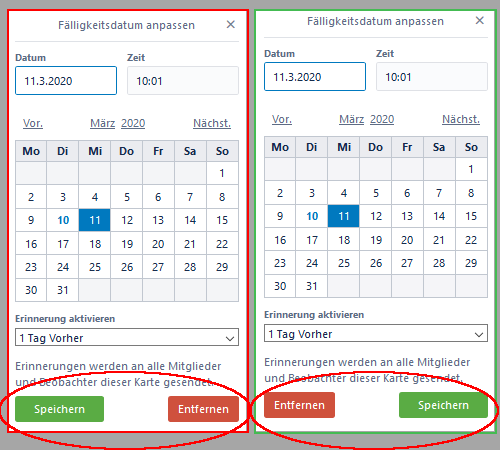
\includegraphics[width=0.5\textwidth]{images/Verbesserungsvorschlaege/1 TrelloDatepicker.PNG}
    \centering
    \caption{Problemgrad 1: Einhaltung des Standards der Leserichtung bei der Platzierung des 'Speichern'-Buttons (Problem Nr. 2, rechts die überarbeitete Version mit dem Button auf der rechten Seite)}
    \label{fig:datepicker}
\end{figure}

\begin{figure}[h]
    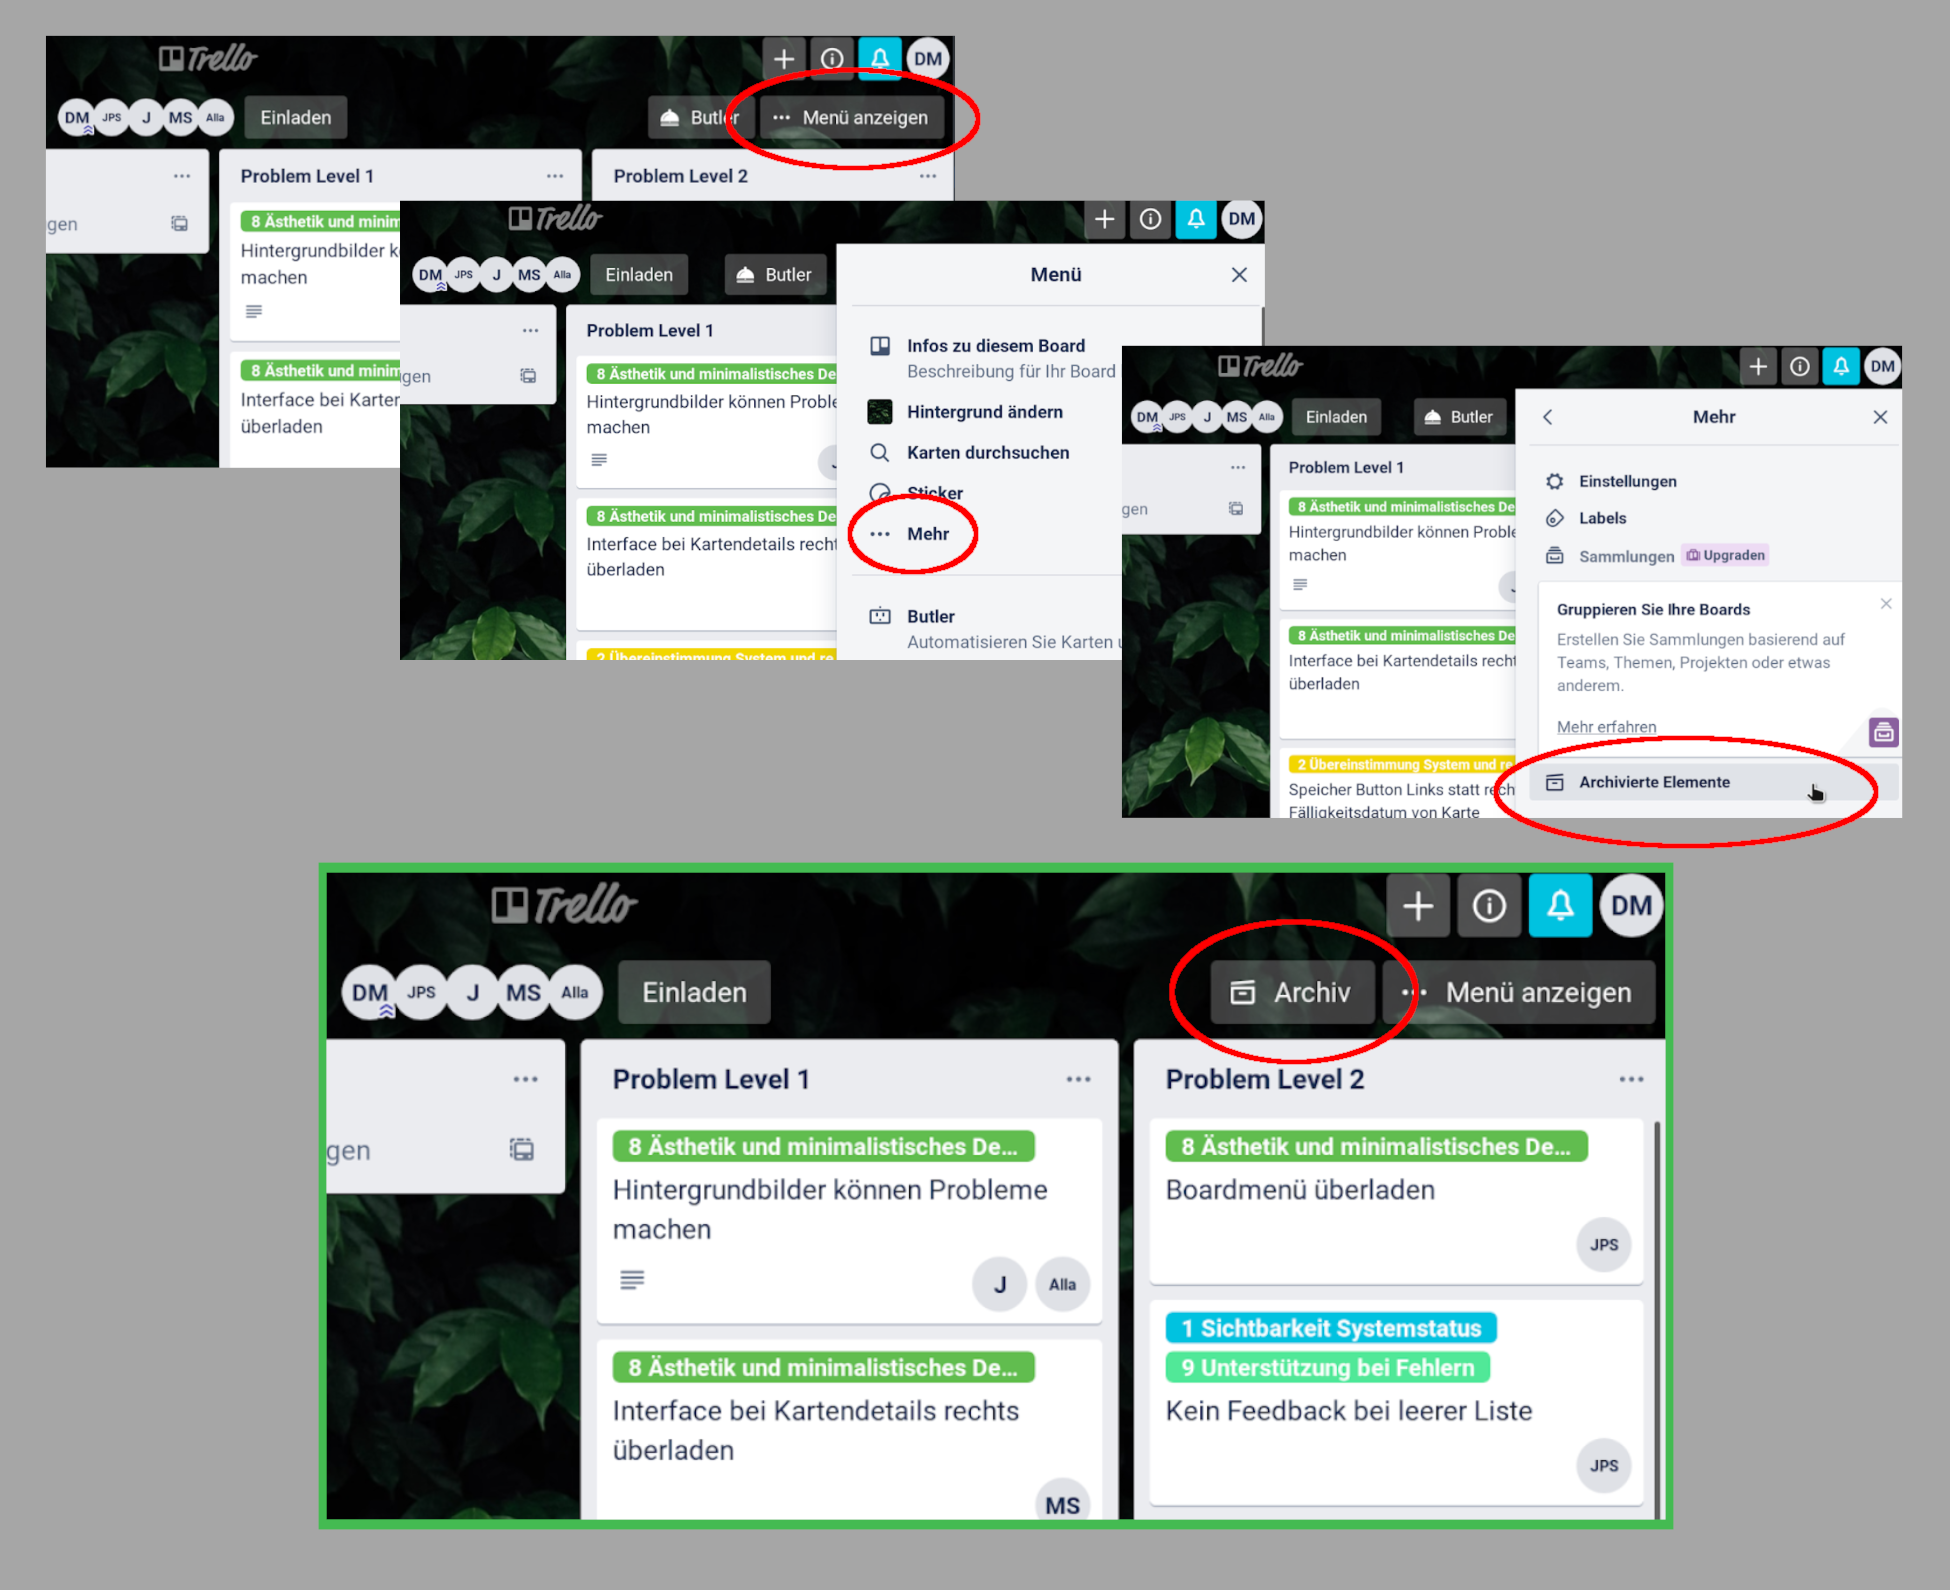
\includegraphics[width=0.9\textwidth]{images/Verbesserungsvorschlaege/2 Archiv.PNG}
    \centering
    \caption{Problemgrad 2: Eine Möglichkeit zum besseren Finden des Archivs (Problem Nr. 15, oben der aktuelle Weg und unten die überarbeitete Version mit eigenem Button)}
    \label{fig:archiv}
\end{figure}

\begin{figure}[h]
    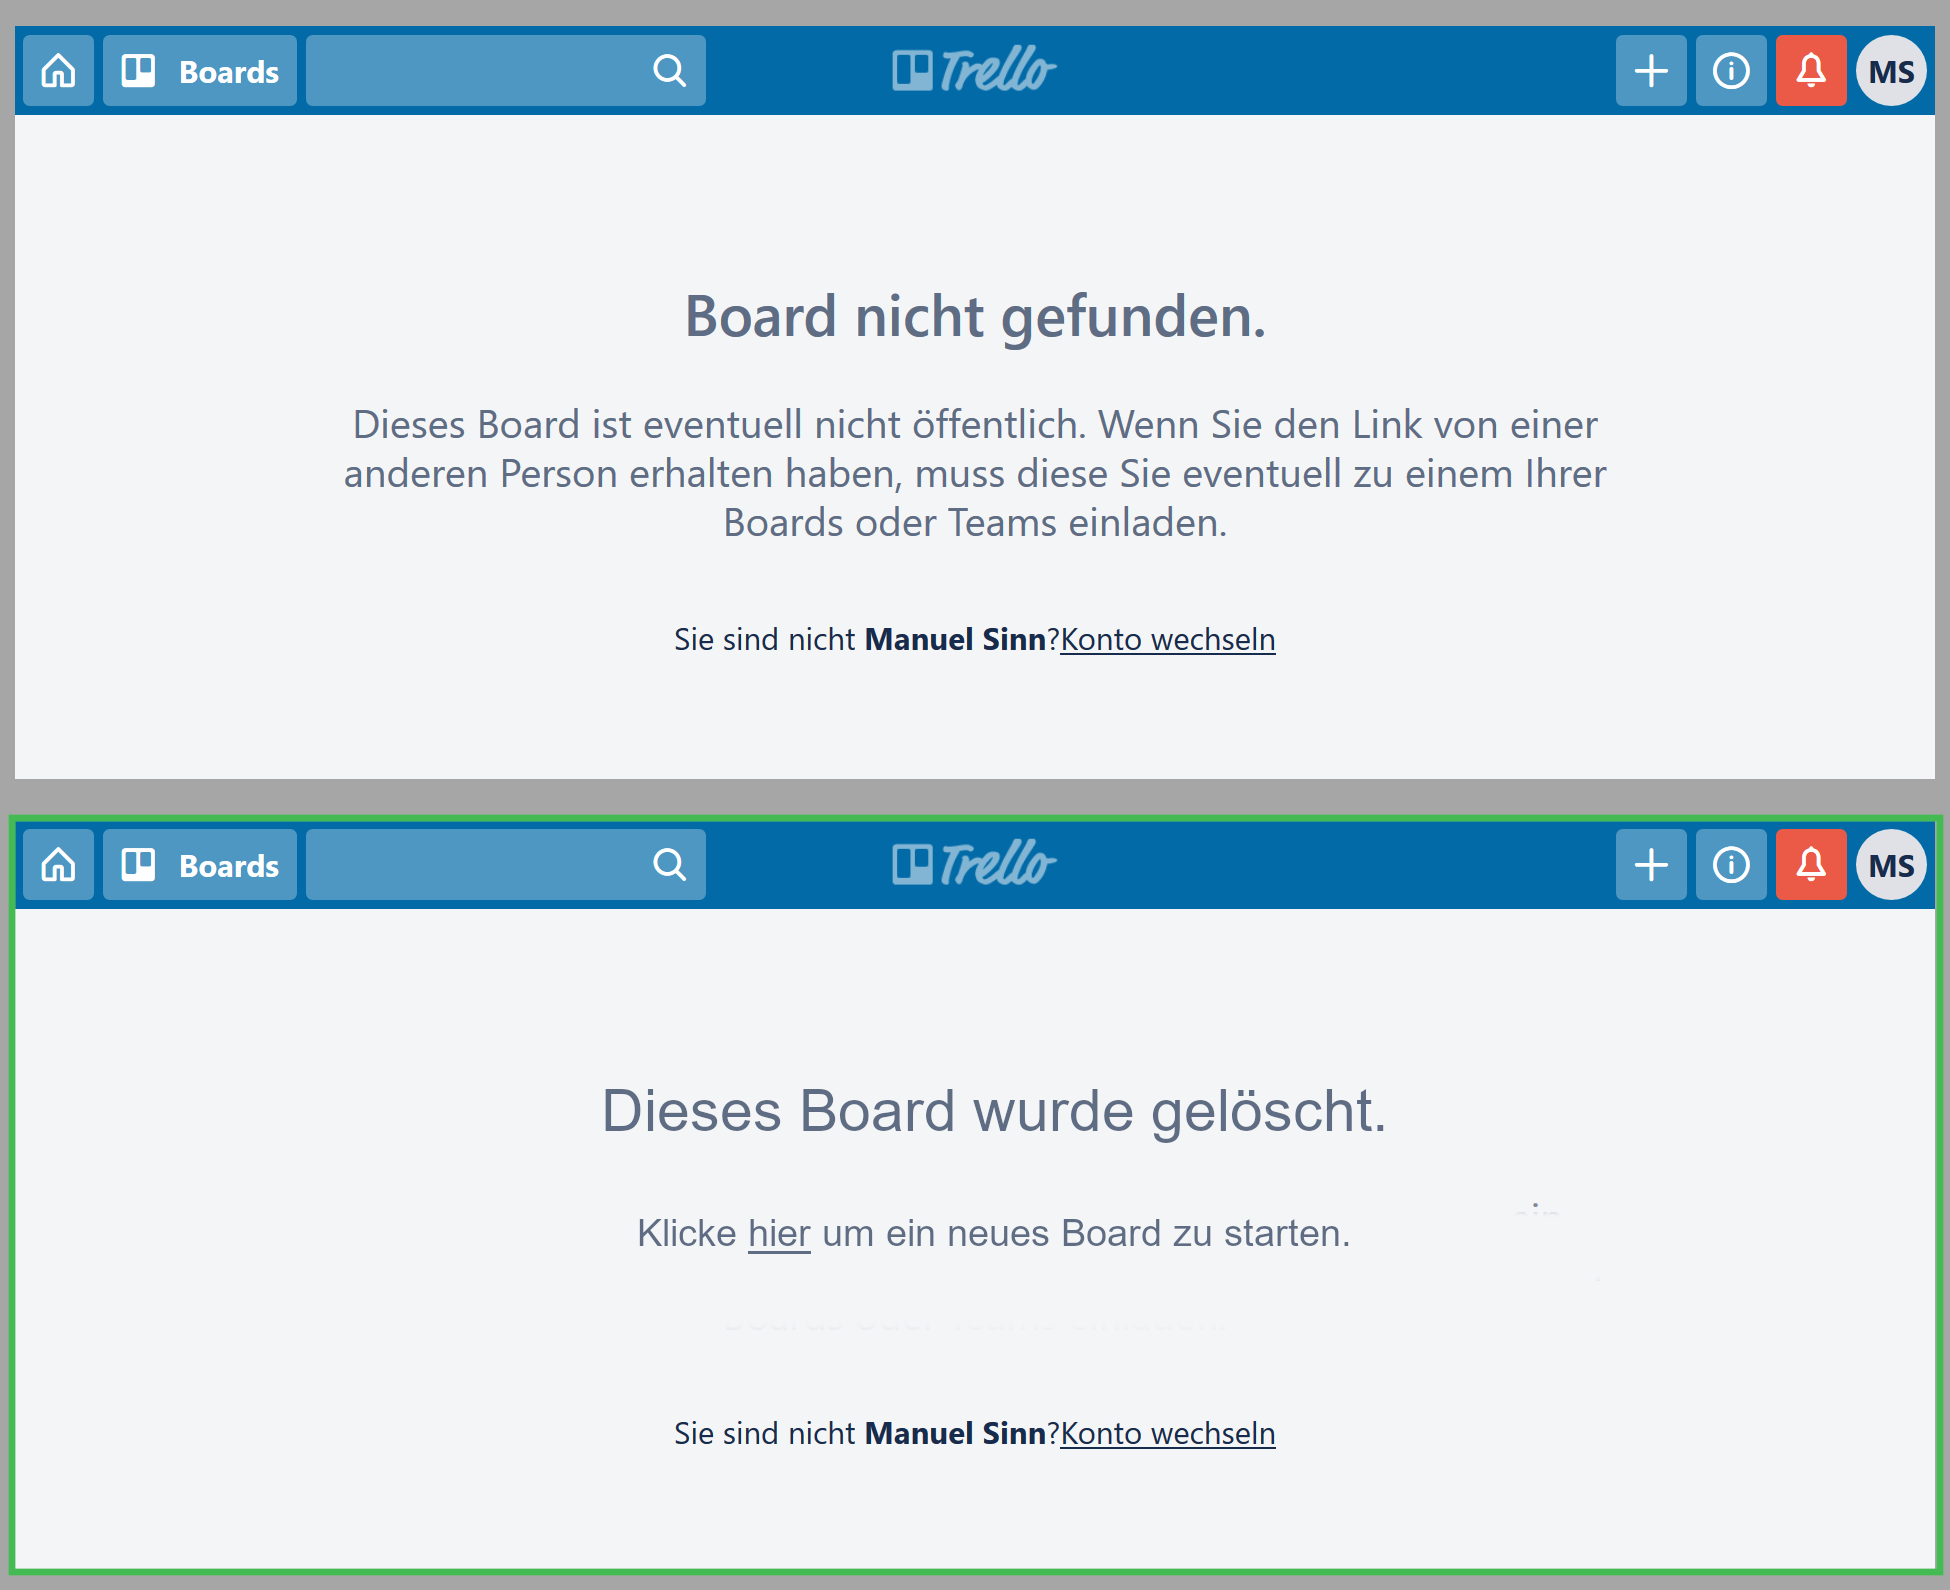
\includegraphics[width=0.7\textwidth]{images/Verbesserungsvorschlaege/3 BoardNichtGefunden.PNG}
    \centering
    \caption{Problemgrad 3: Verbesserung des verwirrenden Feedbacks nach dem endgültigem Löschen eines Boards (Problem Nr. 20, unten die überarbeitete Version)}
    \label{fig:feedback}
\end{figure}

\begin{figure}[h]   
    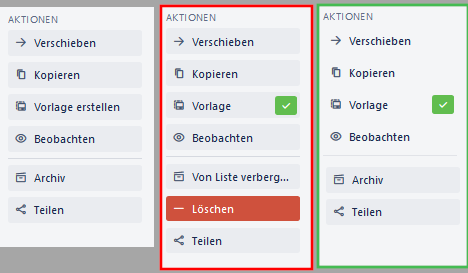
\includegraphics[width=0.6\textwidth]{images/Verbesserungsvorschlaege/4 VorlageErstellen.png}
    \centering
    \caption{Problemgrad 4: Konstanthalten des Menüs statt dem unnötig verwirrendem Verändern bei Wählen der Option 'Vorlage erstellen' (Problem Nr. 9, links die Ausgangssituation, in der Mitte die aktuelle und rechts die überarbeitete Version)}
    \label{fig:vorlage}
\end{figure}
\FloatBarrier




\subsection{Vebesserungsvorschläge Zenkit}
\FloatBarrier
\begin{figure}[h] 
    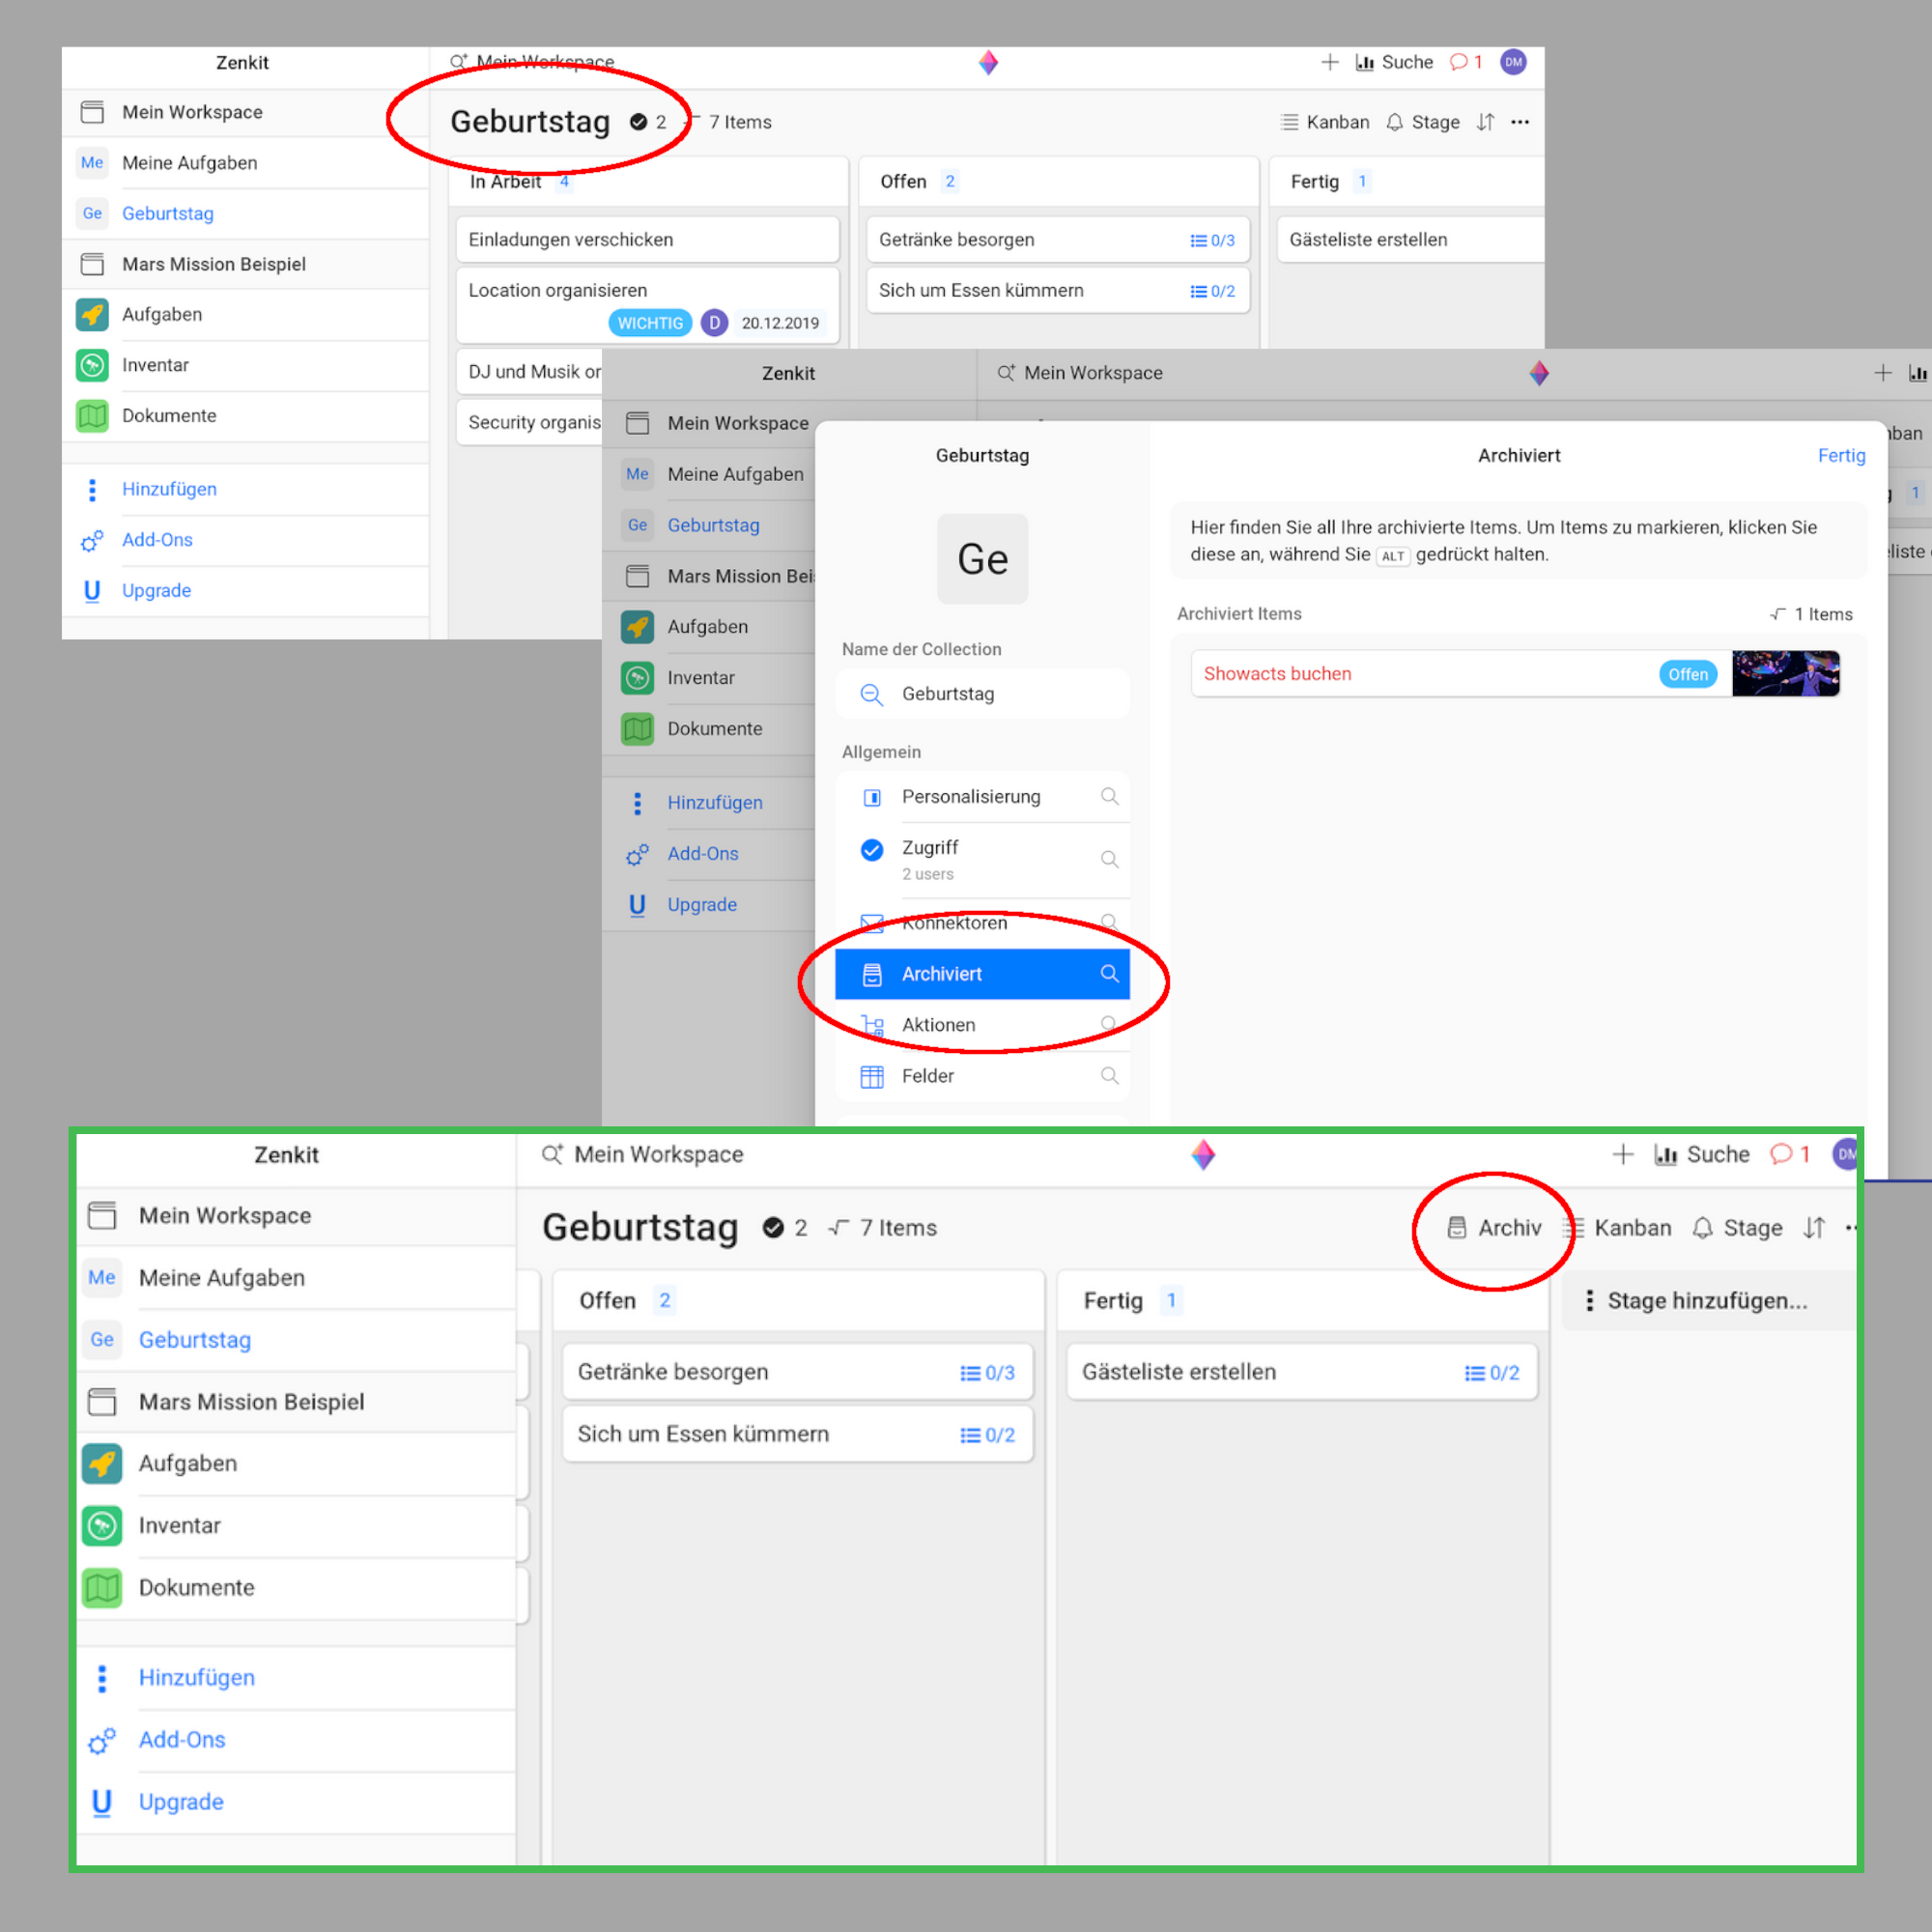
\includegraphics[width=0.6\textwidth]{images/Verbesserungsvorschlaege/zenkitArchiv.png}
    \centering
    \caption{Problemgrad 3, Analog zur Lösung bei Trello, eine Möglichkeit zum besseren Finden des Archivs (Problem Nr. 19, oben der aktuelle Weg und unten die überarbeitete Version mit eigenem Button)}
    \label{fig:zenkitarchiv}
\end{figure}

\begin{figure}[h]   
    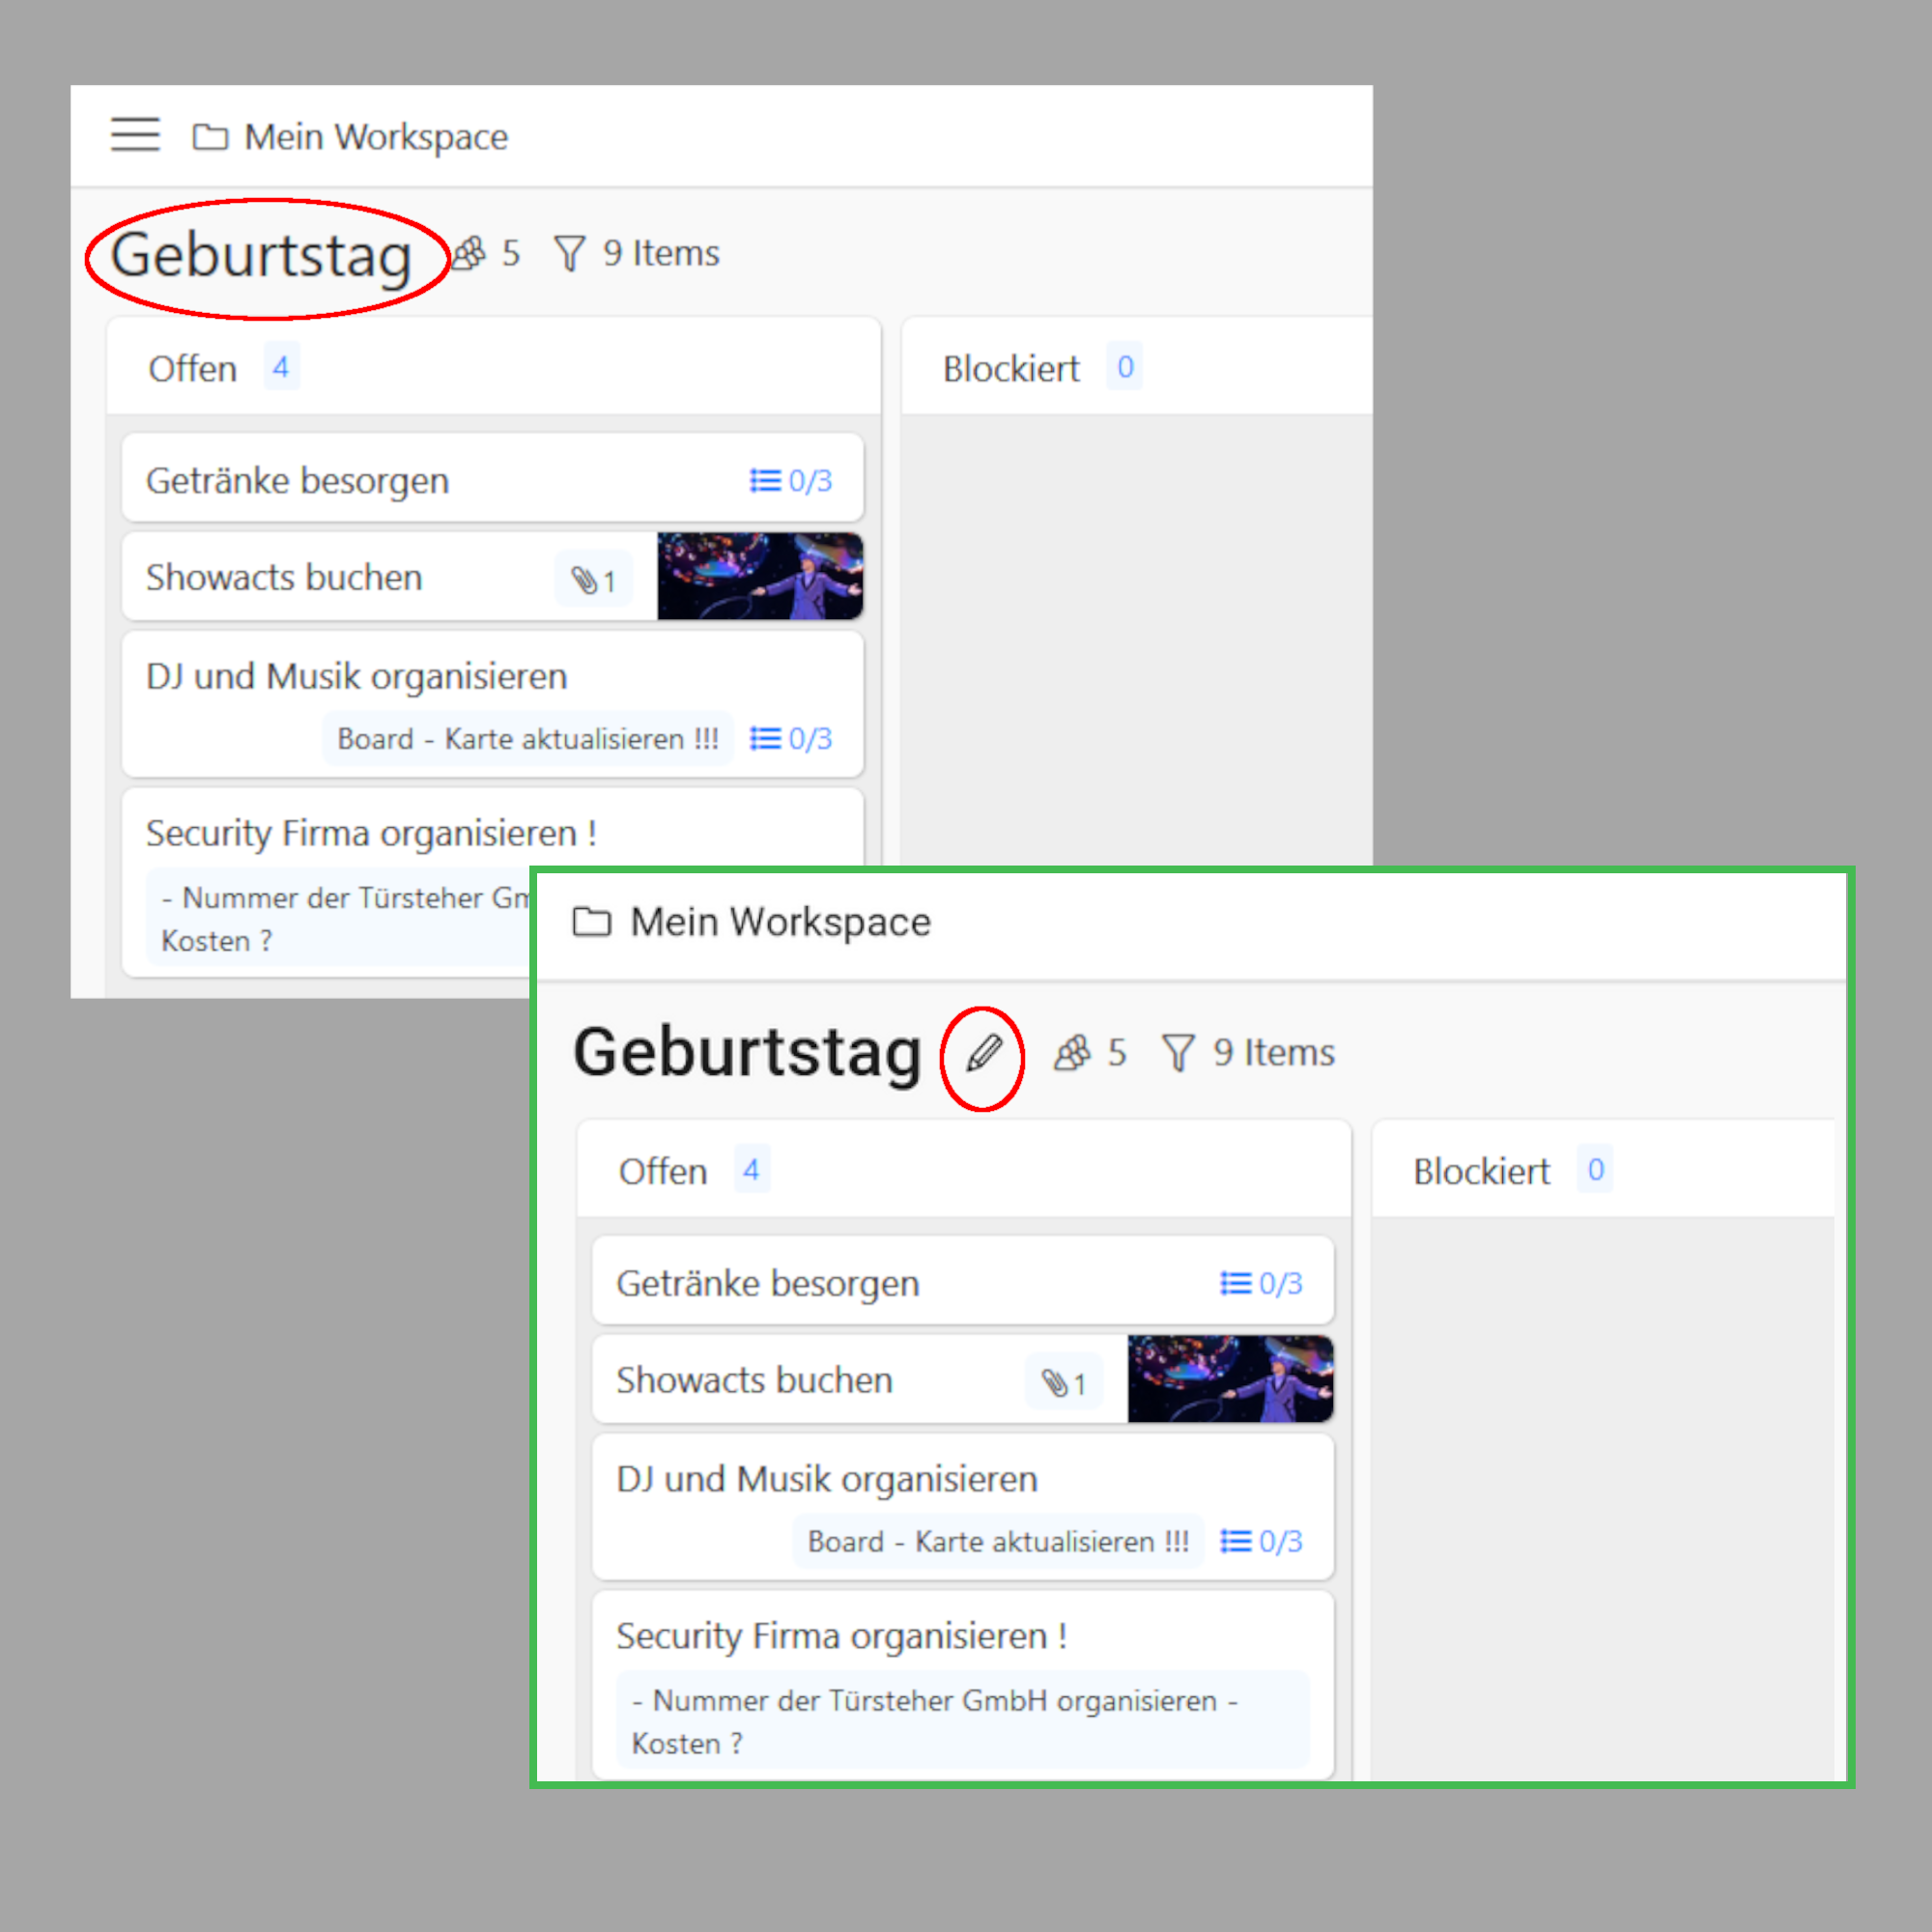
\includegraphics[width=0.6\textwidth]{images/Verbesserungsvorschlaege/ZenkitButton.png}
    \centering
    \caption{Problemgrad 3, Überarbeitung eines für Zenkit typischen Problems, des Versteckens von Bedienelementen (Problem Nr. 20). Der Button für weitere Optionen ist im Namen der Collection 'versteckt', daher wurde in der überarbeiteten Version unten ein eigener Button zum Aufrufen dieser Einstellungen eingefügt.}
    \label{fig:zenkitbutton}
\end{figure}

\begin{figure}[h]
    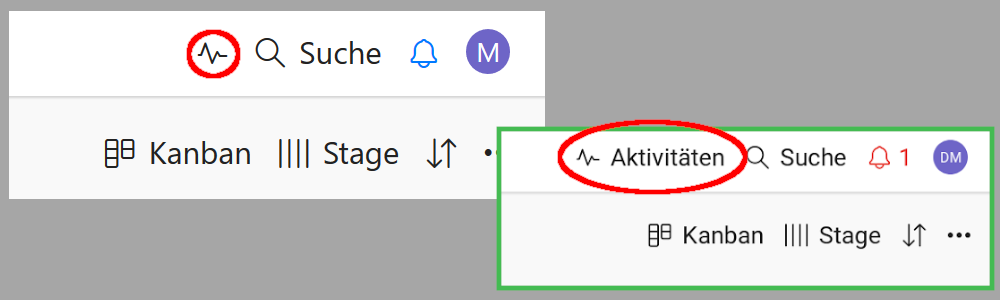
\includegraphics[width=0.6\textwidth]{images/Verbesserungsvorschlaege/zenkitActivities.png}
    \centering
    \caption{Problemgrad 1, Überarbeitung des Aktivitätenbuttons, da dieser schwer aufzufinden und interpretieren war (Problem Nr. 20). Unten die überarbeitete Version mit klarer Benennung.}
    \label{fig:zenkitaktivit}
\end{figure}

\begin{figure}[h]   
    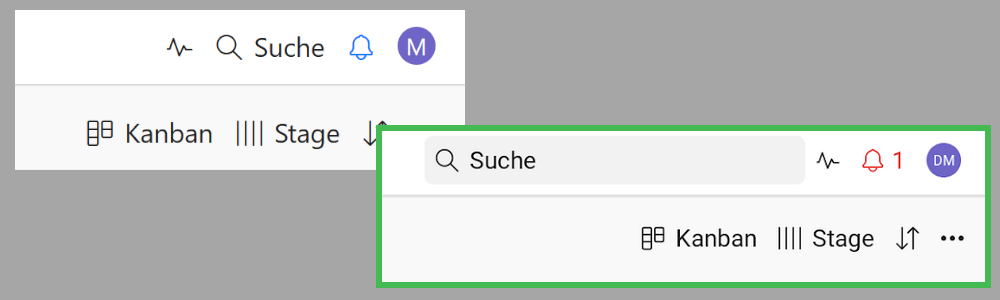
\includegraphics[width=0.6\textwidth]{images/Verbesserungsvorschlaege/zenkitSuche.png}
    \centering
    \caption{Problemgrad 1, Überarbeitung des Suchfeldes, welches, ähnlich wie der Aktivitätenbutton, nicht präsent genug erschien (Problem Nr. 16).}
    \label{fig:zenkitsuche}
\end{figure}

\FloatBarrier
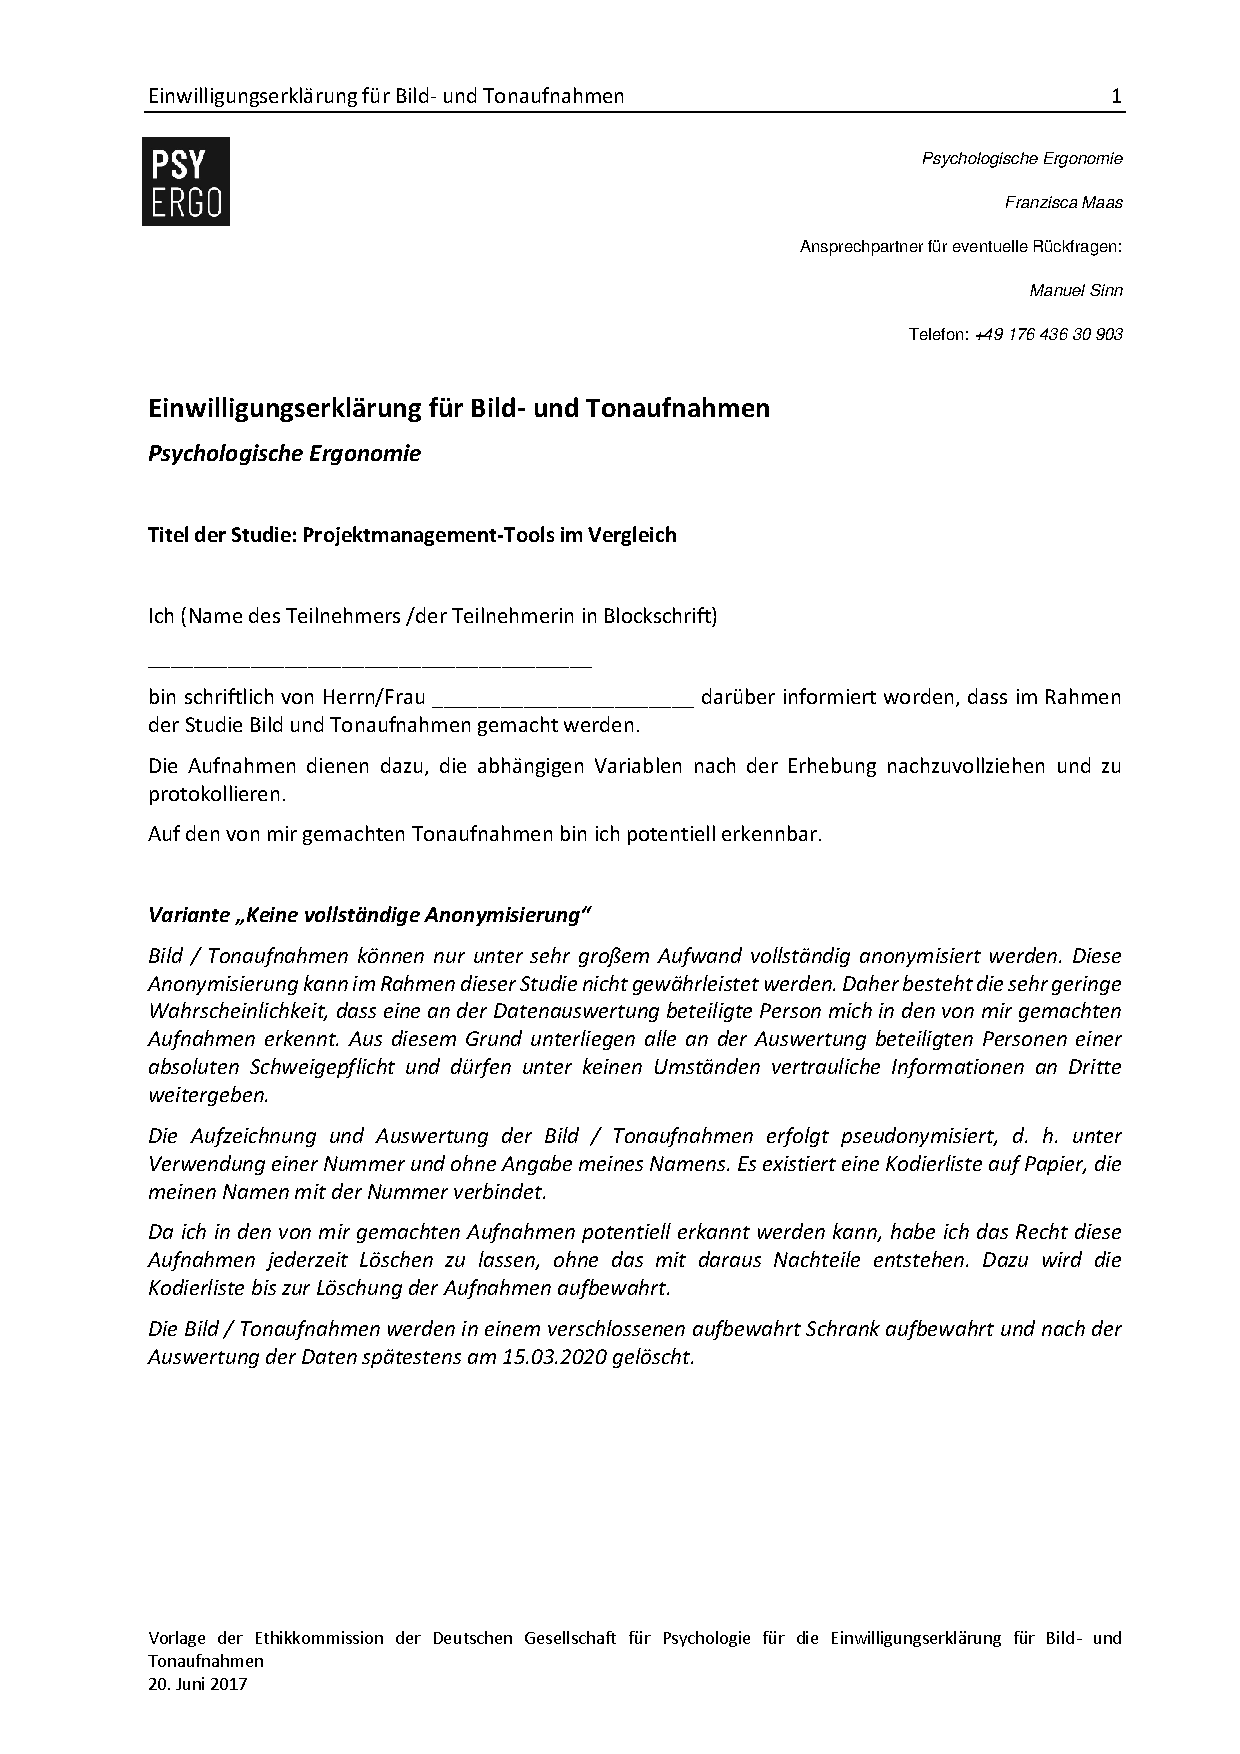
\includepdf[scale=0.8, pages=1,pagecommand=\subsection{Fragebögen}]{images/pdf/bildton.pdf}
\includepdf[scale=0.8, pages=2-,pagecommand={}]{images/pdf/bildton.pdf}

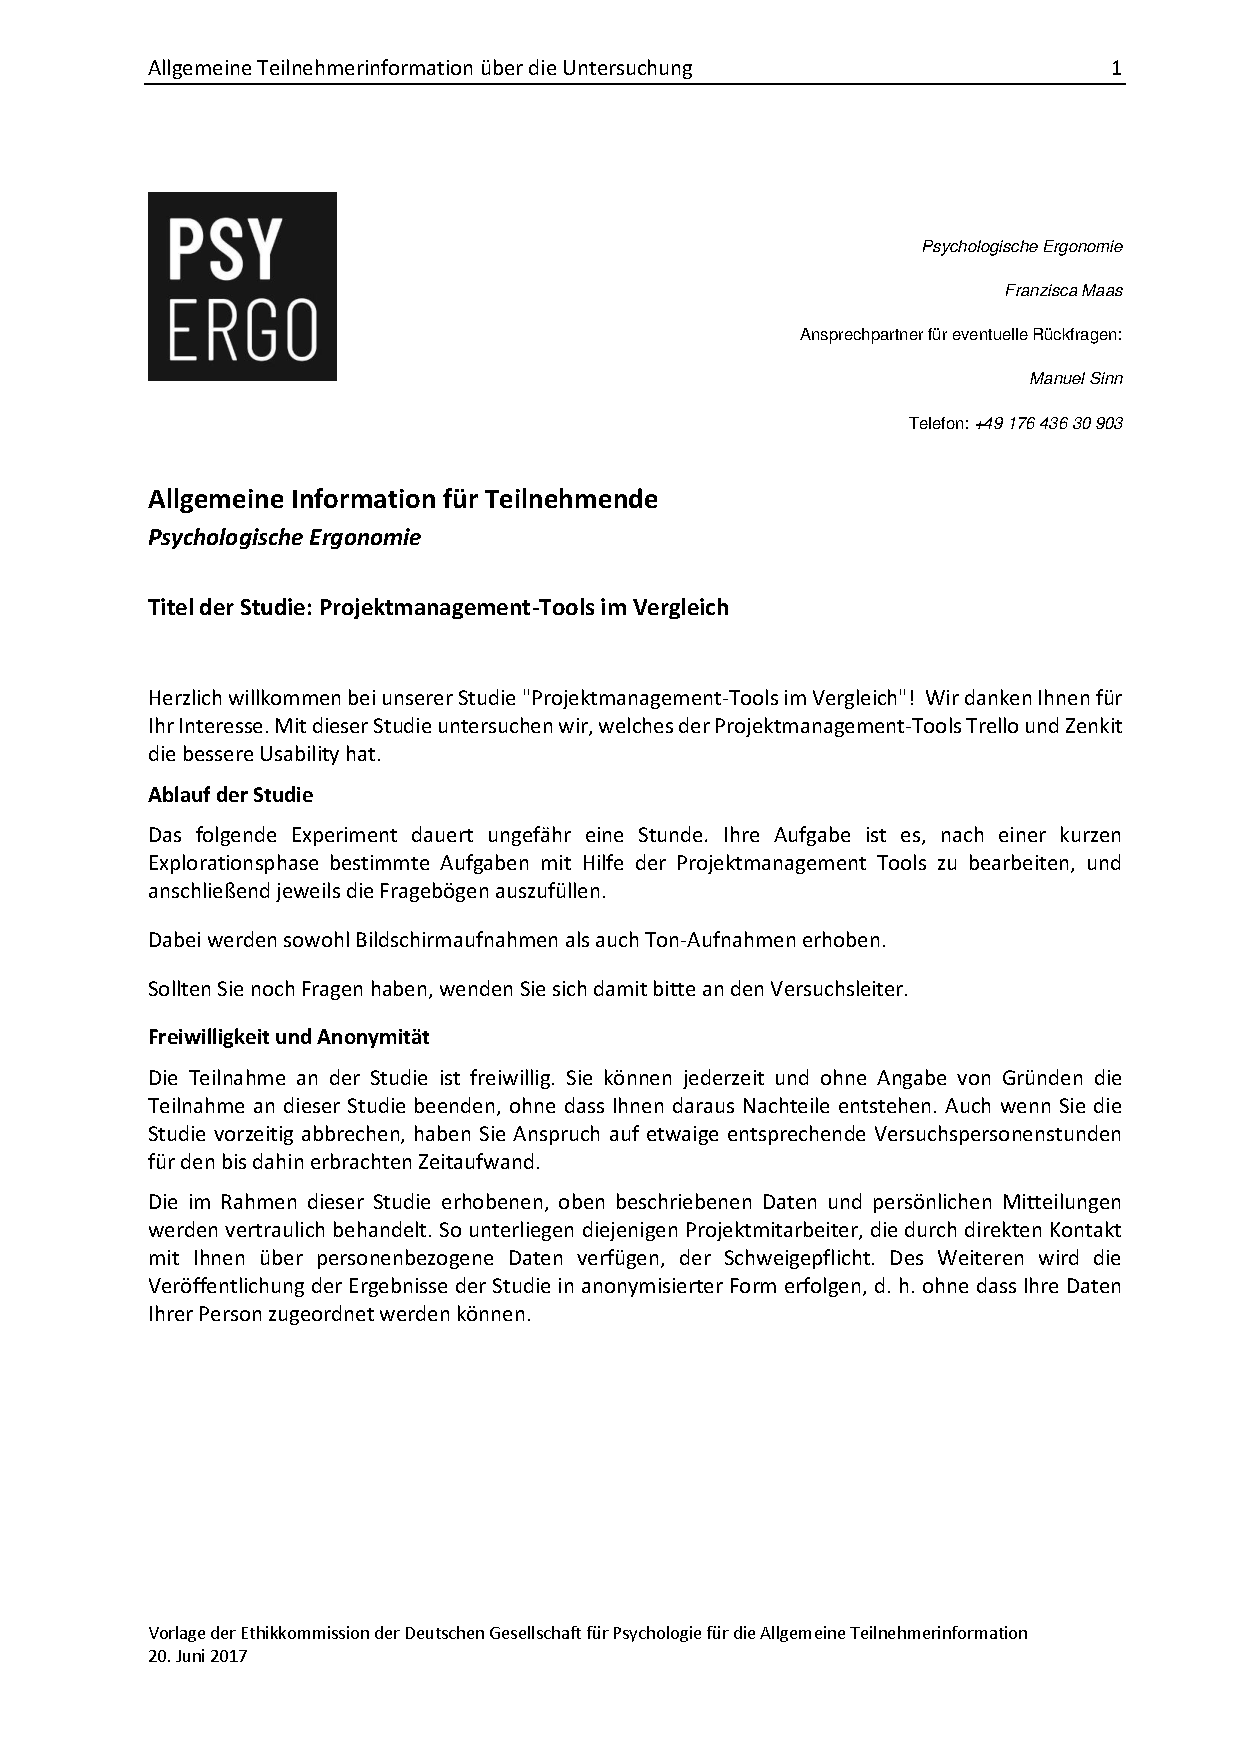
\includepdf[pages=-,scale=.8, pagecommand={}]{images/pdf/Datenschutz.pdf}
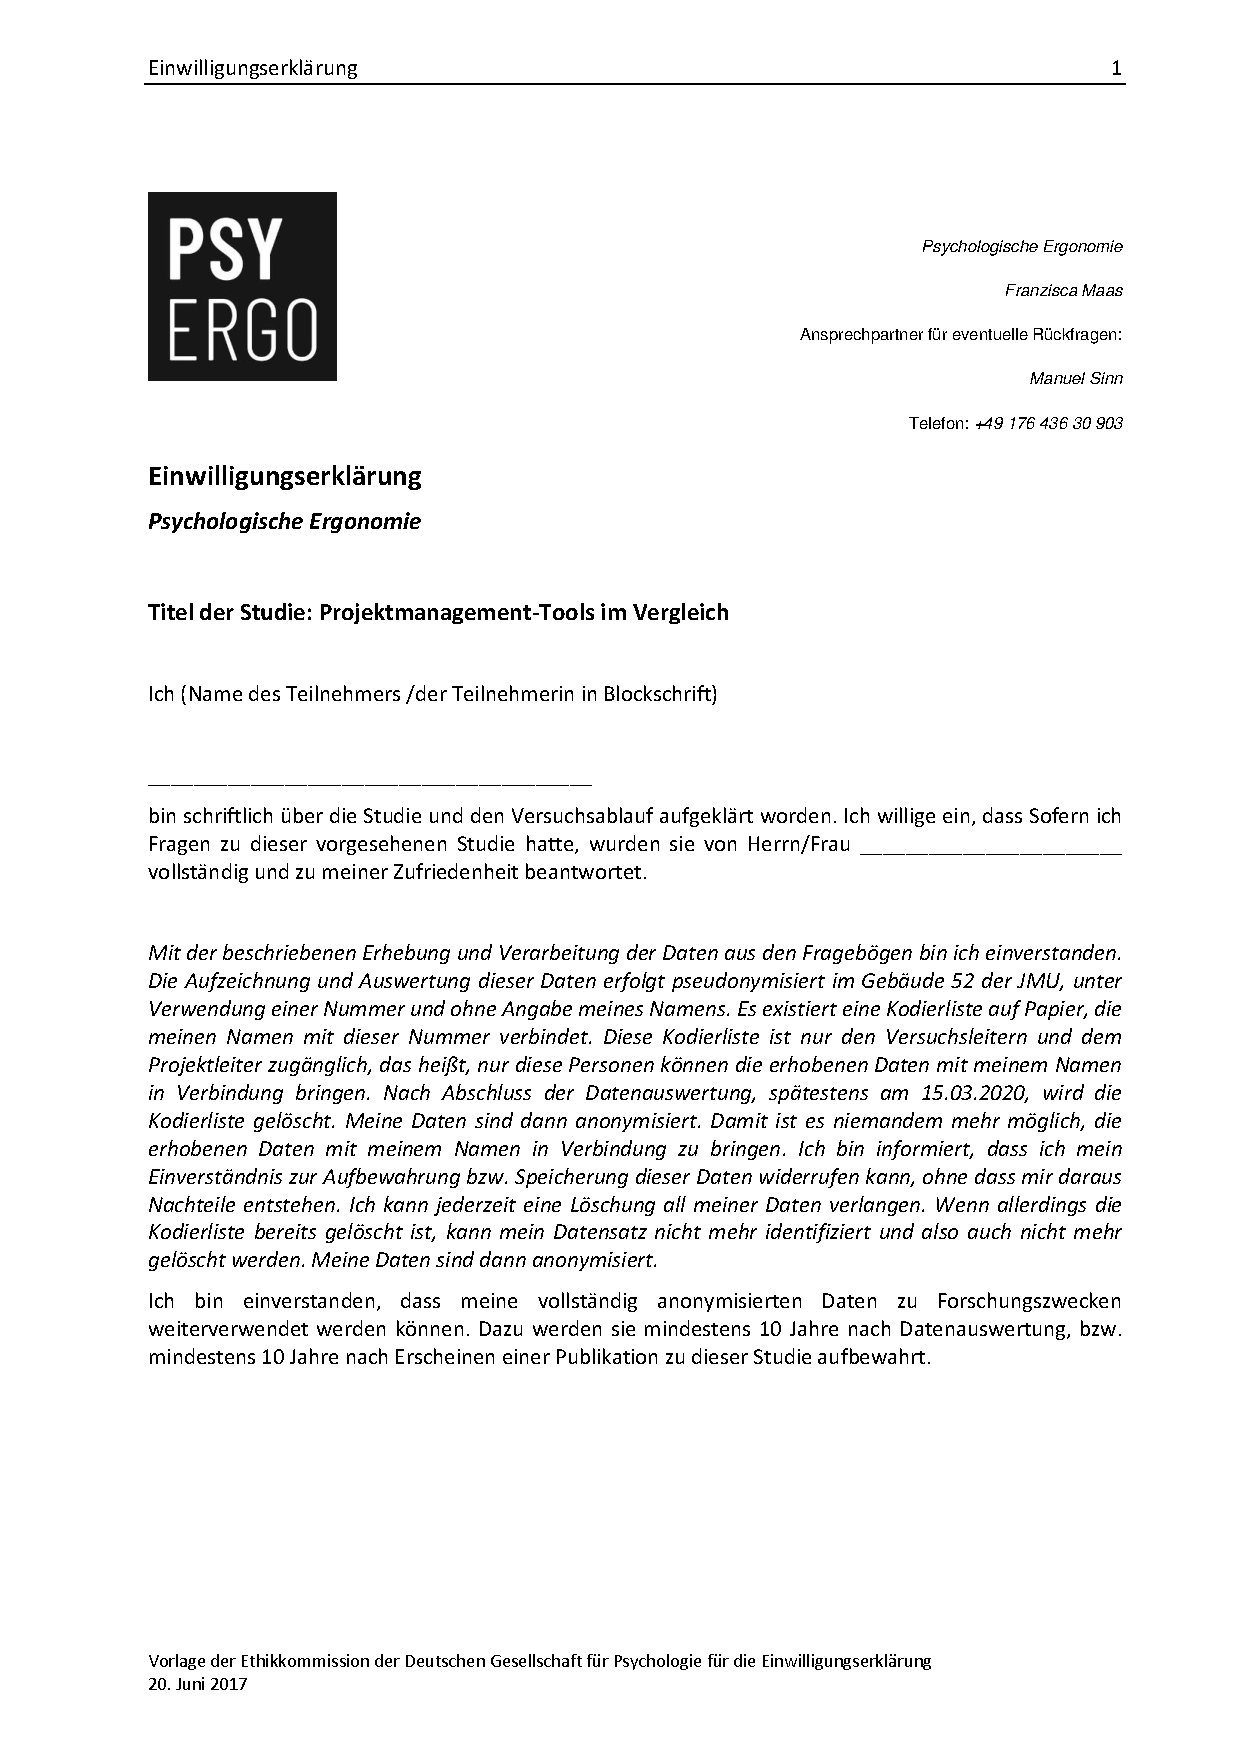
\includepdf[pages=-,scale=.8, pagecommand={}]{images/pdf/Einwilligung.pdf}

\begin{figure}[H]
    \includegraphics[width=0.8\textwidth]{images/Frageboegen/1 Über_Person.PNG}
    \centering
    \caption{Fragebogen zur Erhebung persönlicher Daten}
    \label{fig:person}
\end{figure}

\begin{figure}[H]
    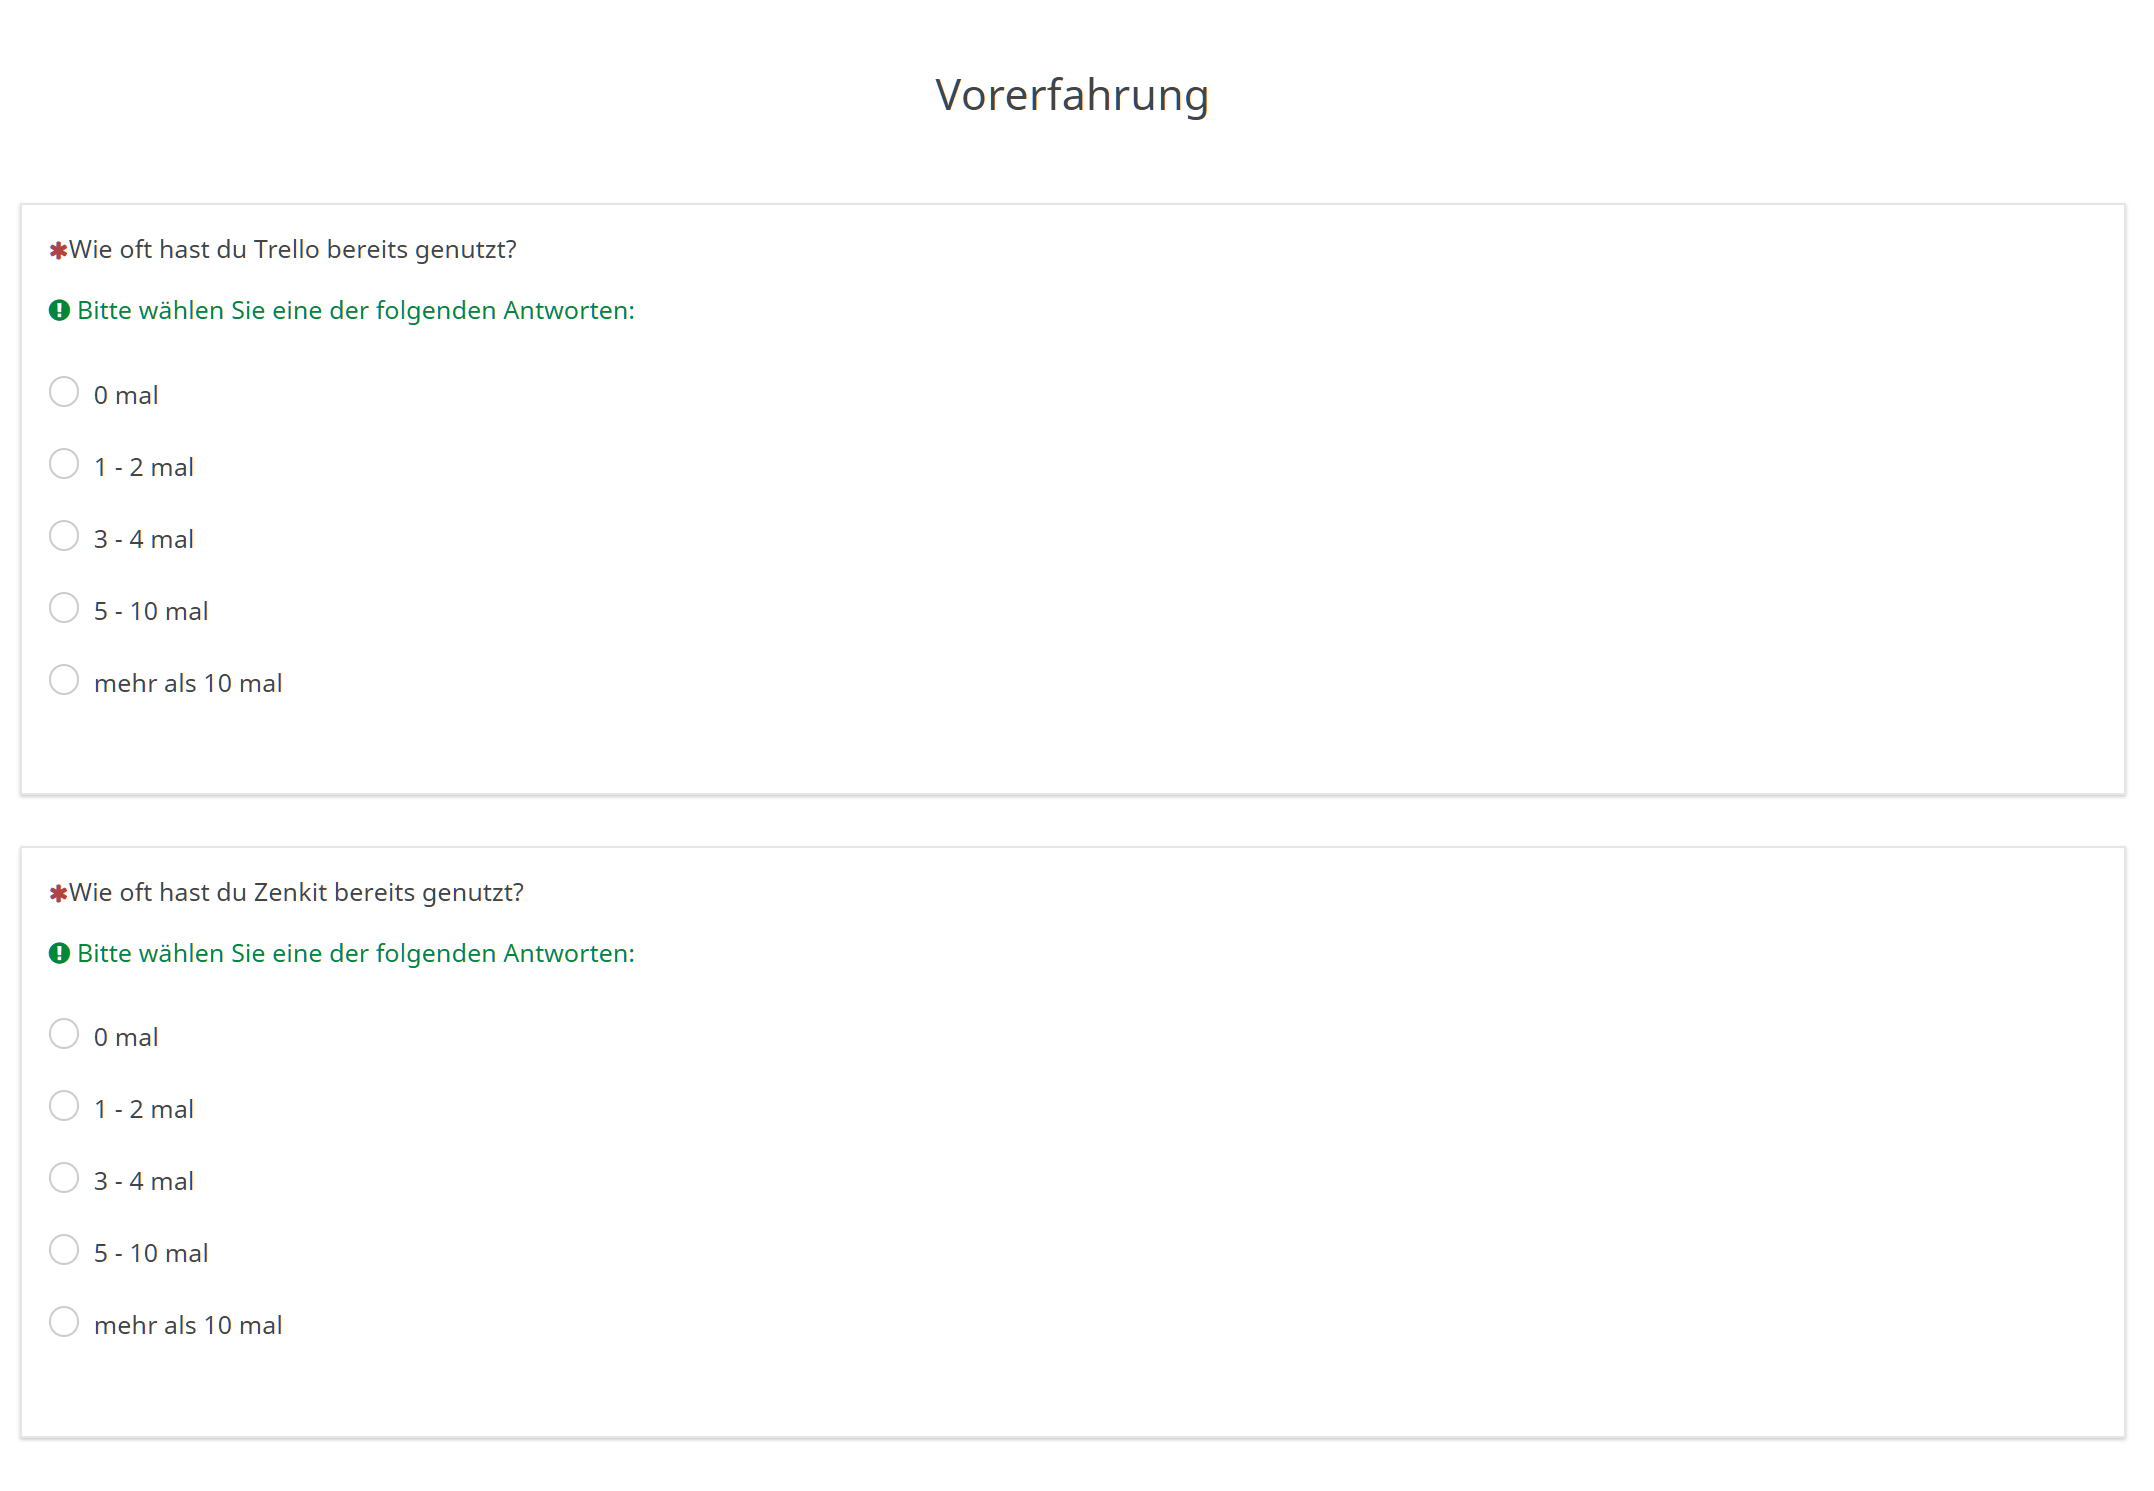
\includegraphics[width=0.8\textwidth]{images/Frageboegen/2 Vorerfahrung.PNG}
    \centering
    \caption{Fragebogen zur Erhebung der Vorerfahrung}
    \label{fig:vorerfahrung}
\end{figure}

\begin{figure}[H]
    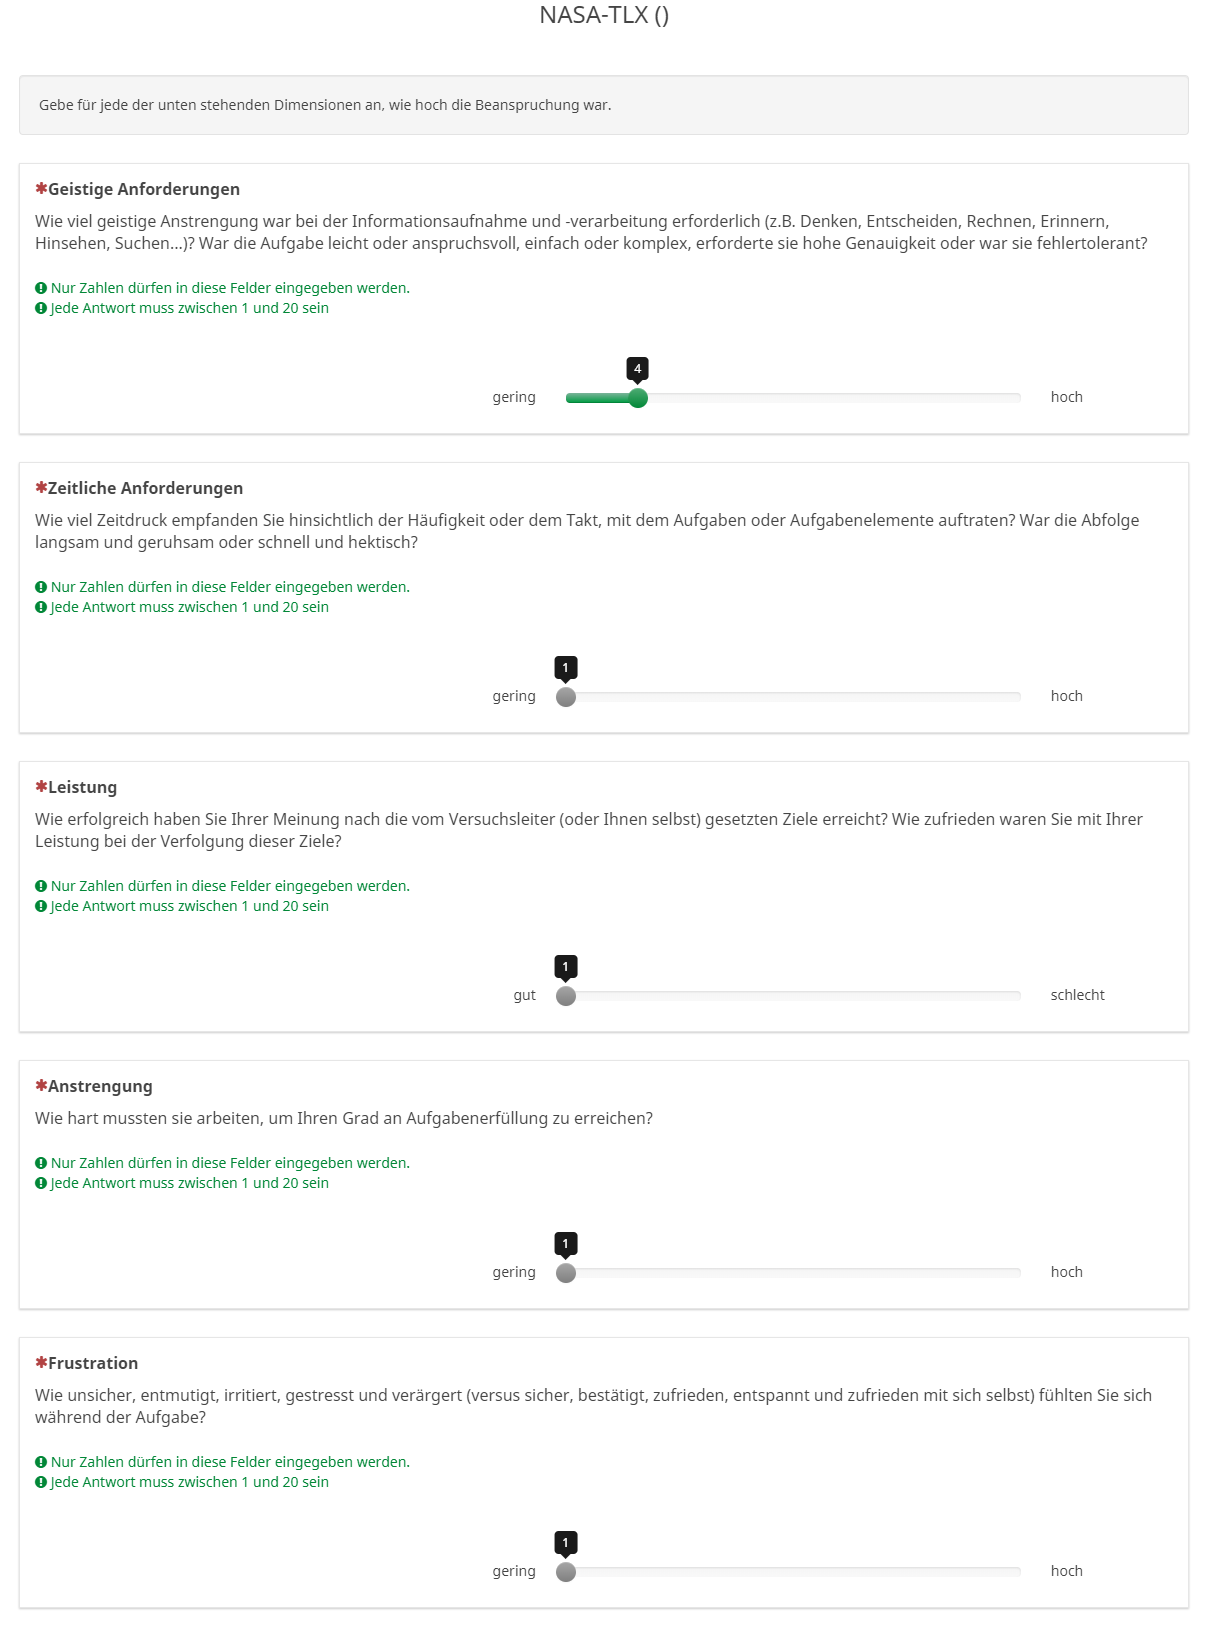
\includegraphics[width=\textwidth]{images/Frageboegen/3 NASA-TLX.PNG}
    \centering
    \caption{NASA TLX Fragebogen für die Erhebung der Effizienz}
    \label{fig:tlx}
\end{figure}

\begin{figure}[H]
    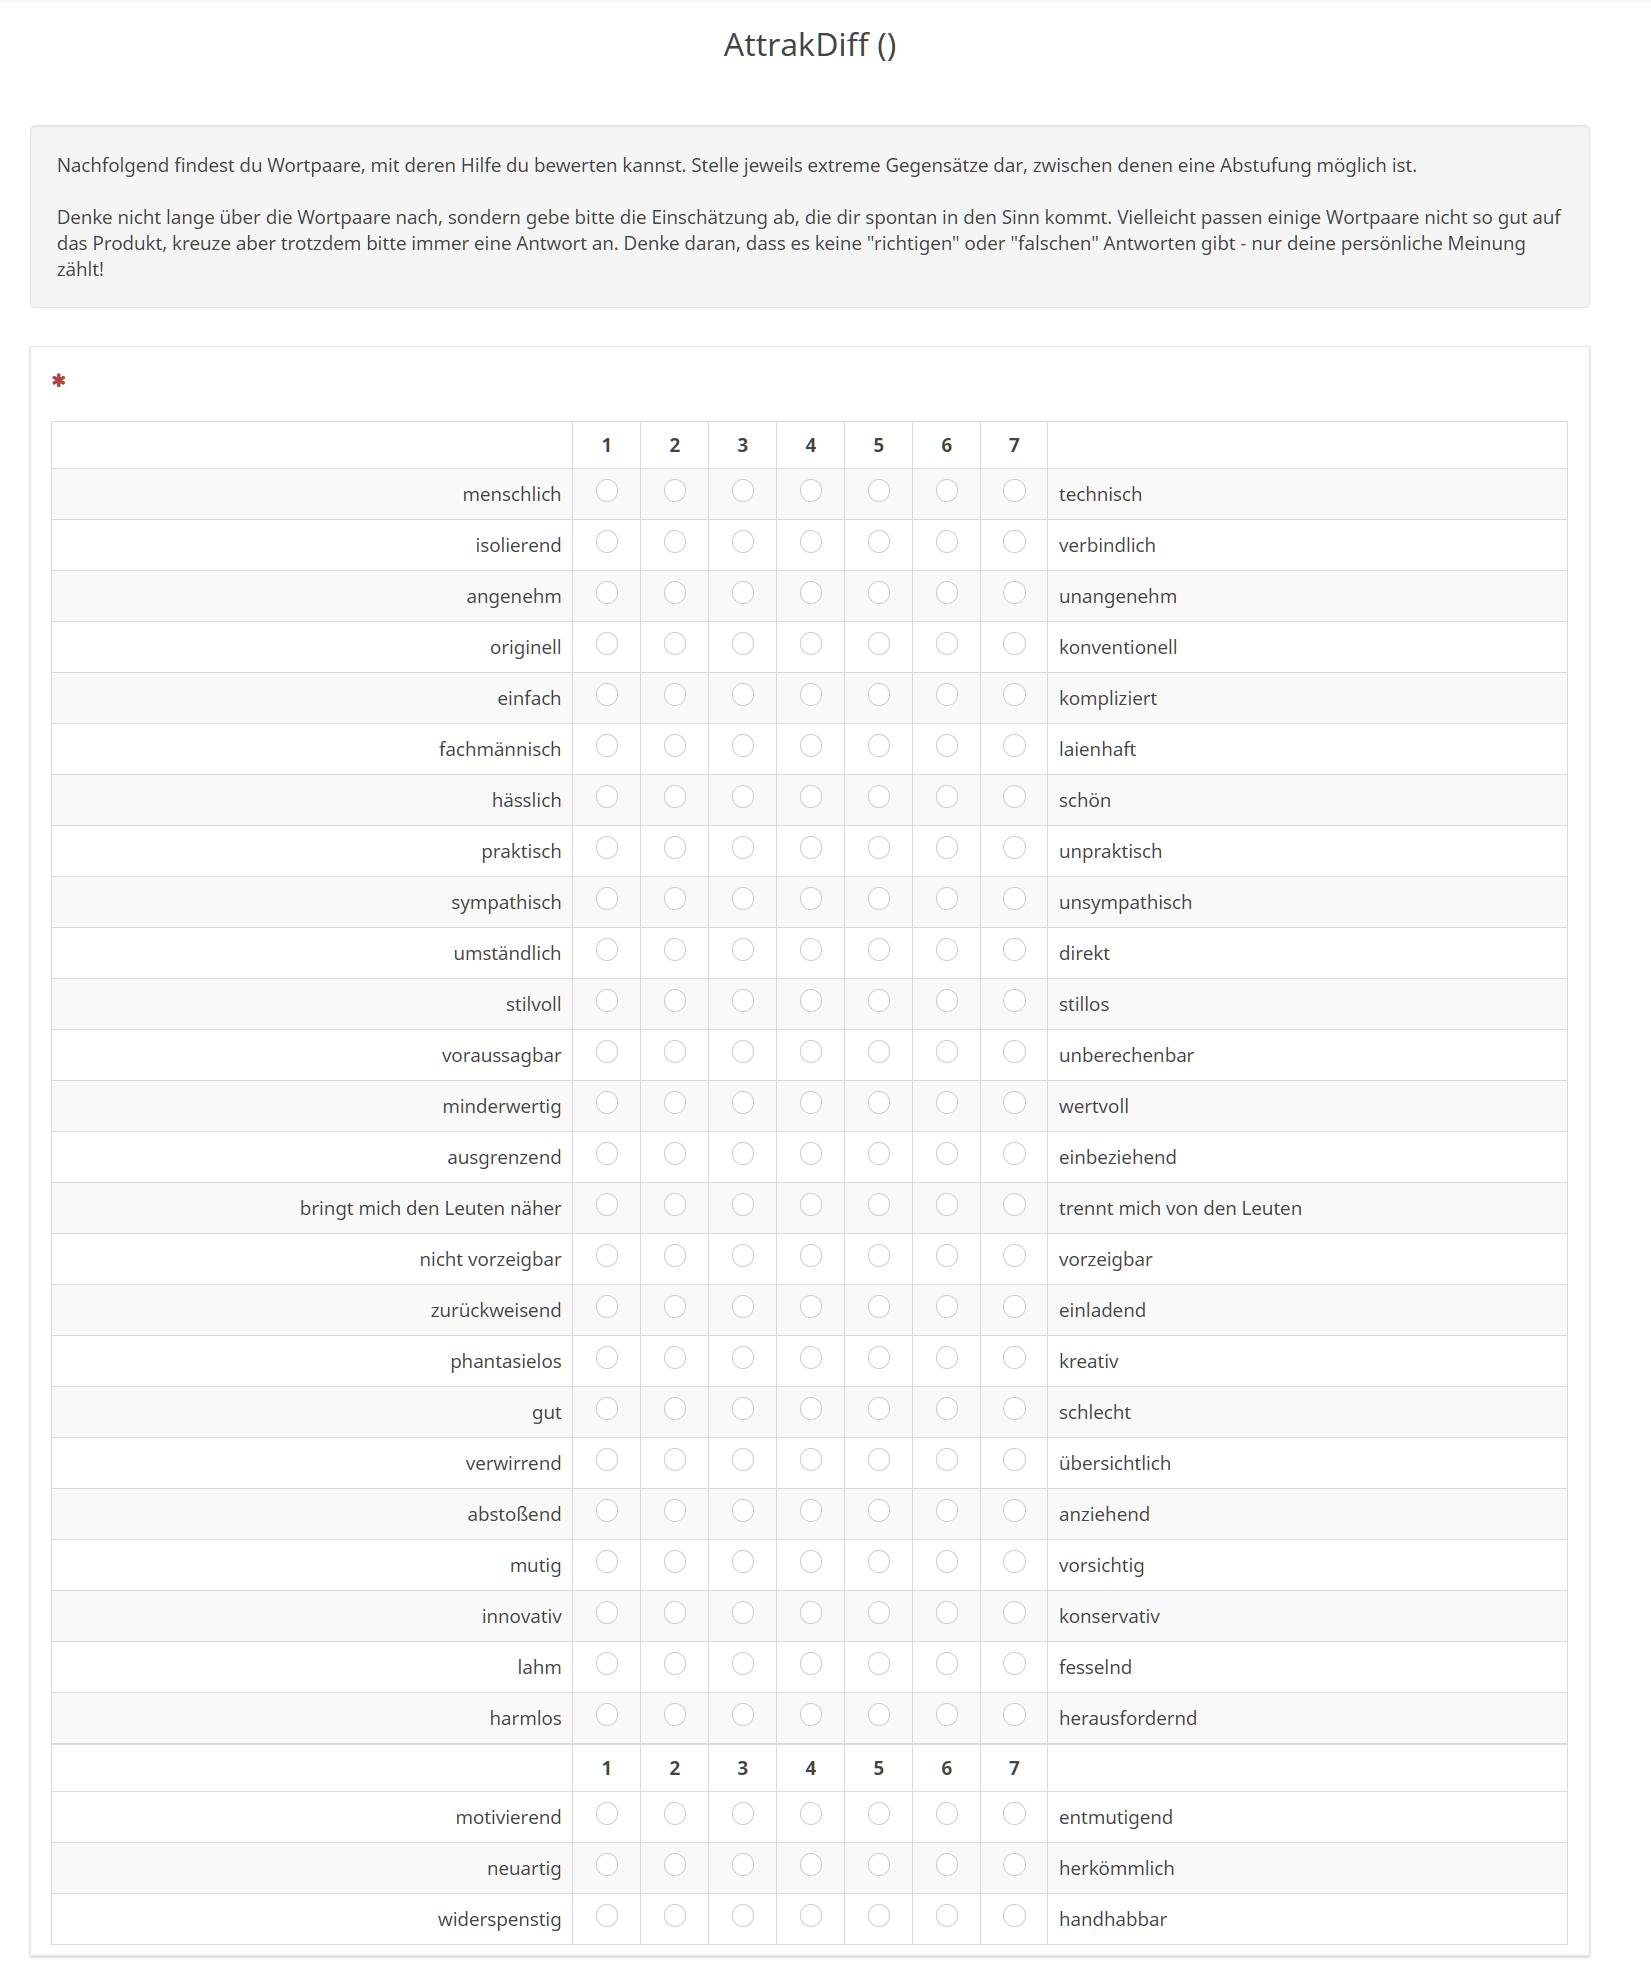
\includegraphics[width=\textwidth]{images/Frageboegen/4 ADiff.PNG}
    \centering
    \caption{AttrakDiff Fragebogen für die Erhebung der Zufriedenheit}
    \label{fig:adiff}
\end{figure}

\includepdf[pages=2-3,scale=.8, nup=1x2, pagecommand=\subsection{Aufgaben}]{images/pdf/aufgabenfolien}

\includepdf[pages=4-,scale=.8, nup=1x2, pagecommand={}]{images/pdf/aufgabenfolien}


\subsubsection{Teilung der Aufgaben in Unteraufgaben zur Berechnung des Effektivitätsmaßes}

\begin{outline}[enumerate]
\newline
Aufgabe 1:\\
1. Karte mit richtiger Bezeichnung erstellen\\
2. Frist auf eine Woche festlegen\\
3. David assignen\\

\\Aufgabe 2:\\
4. Karte nach in Arbeit verschieben\\  
5. Erstes Item auf Checkliste abhaken\\
6. Zweites Item auf Checkliste abhaken\\

\\Aufgabe 3:\\
7. Eltern Karte archivieren\\  
8. Liste archivieren/löschen\\
9. Oma-Karte archivieren\\

\\Aufgabe 4:\\
10. Karte erstellen mit akkurater Bezeichnung\\
11. Checkliste erstellen\\
12. Checklist Items hinzufügen\\

\\Aufgabe 5:\\
13. Karte aus dem Archiv wiederherstellen\\
14. Karte in 'In Arbeit' verschieben\\
15. Farbliche Hervorhebung\\
\end{outline}

\begin{figure}[H]
    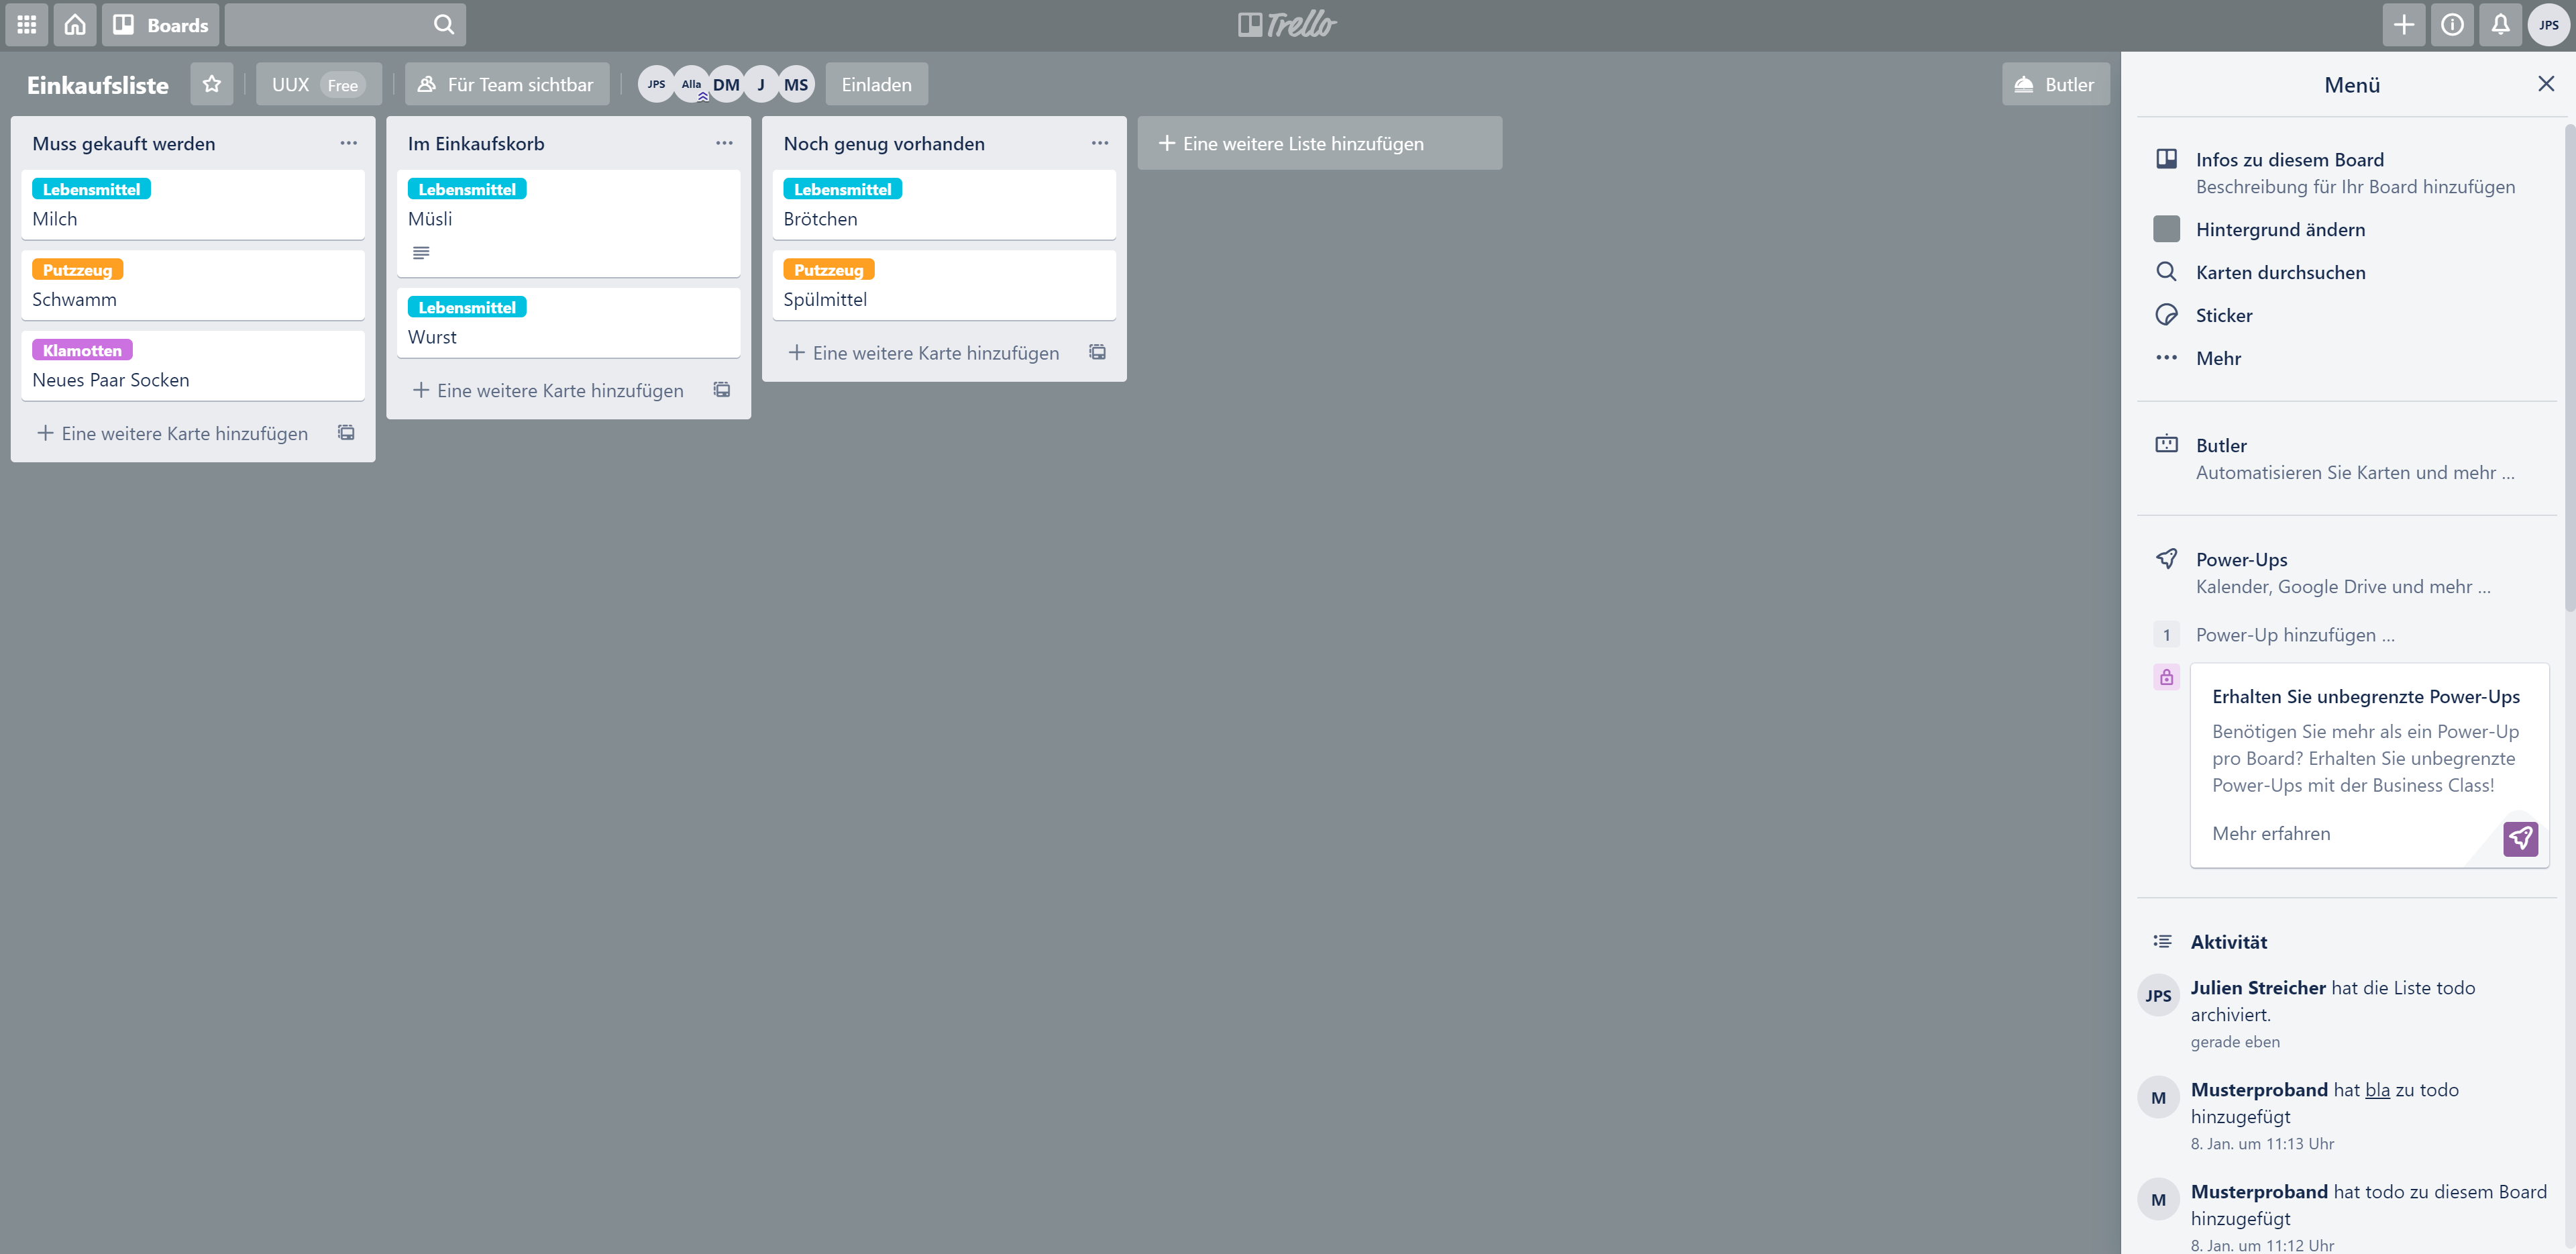
\includegraphics[width=\textwidth]{images/UI/Einkaufsliste.PNG}
    \centering
    \caption{Vorlagenboard 'Einkaufsliste' bei Trello}
    \label{fig:trelloeinkauf}
\end{figure}

\begin{figure}[H]
    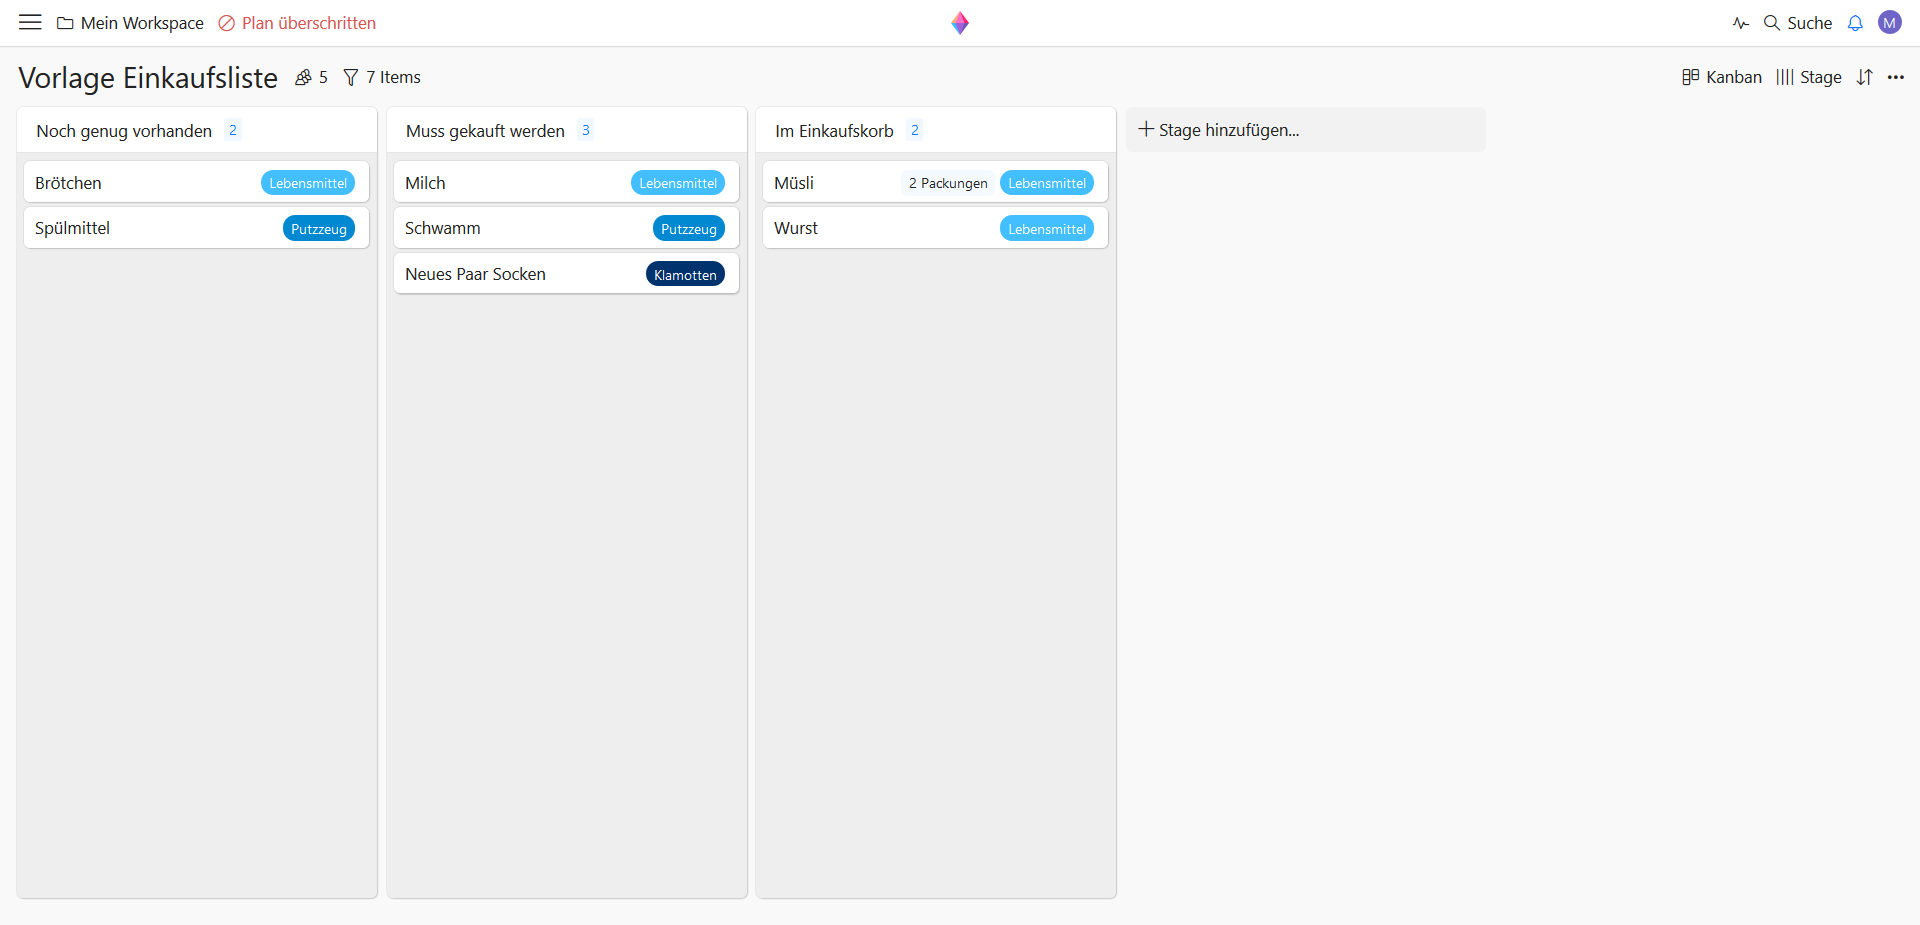
\includegraphics[width=\textwidth]{images/UI/zenkiteinkaufsliste.PNG}
    \centering
    \caption{Vorlagenboard 'Einkaufsliste' bei Zenkit}
    \label{fig:zenkiteinkauf}
\end{figure}

\begin{figure}[H]
    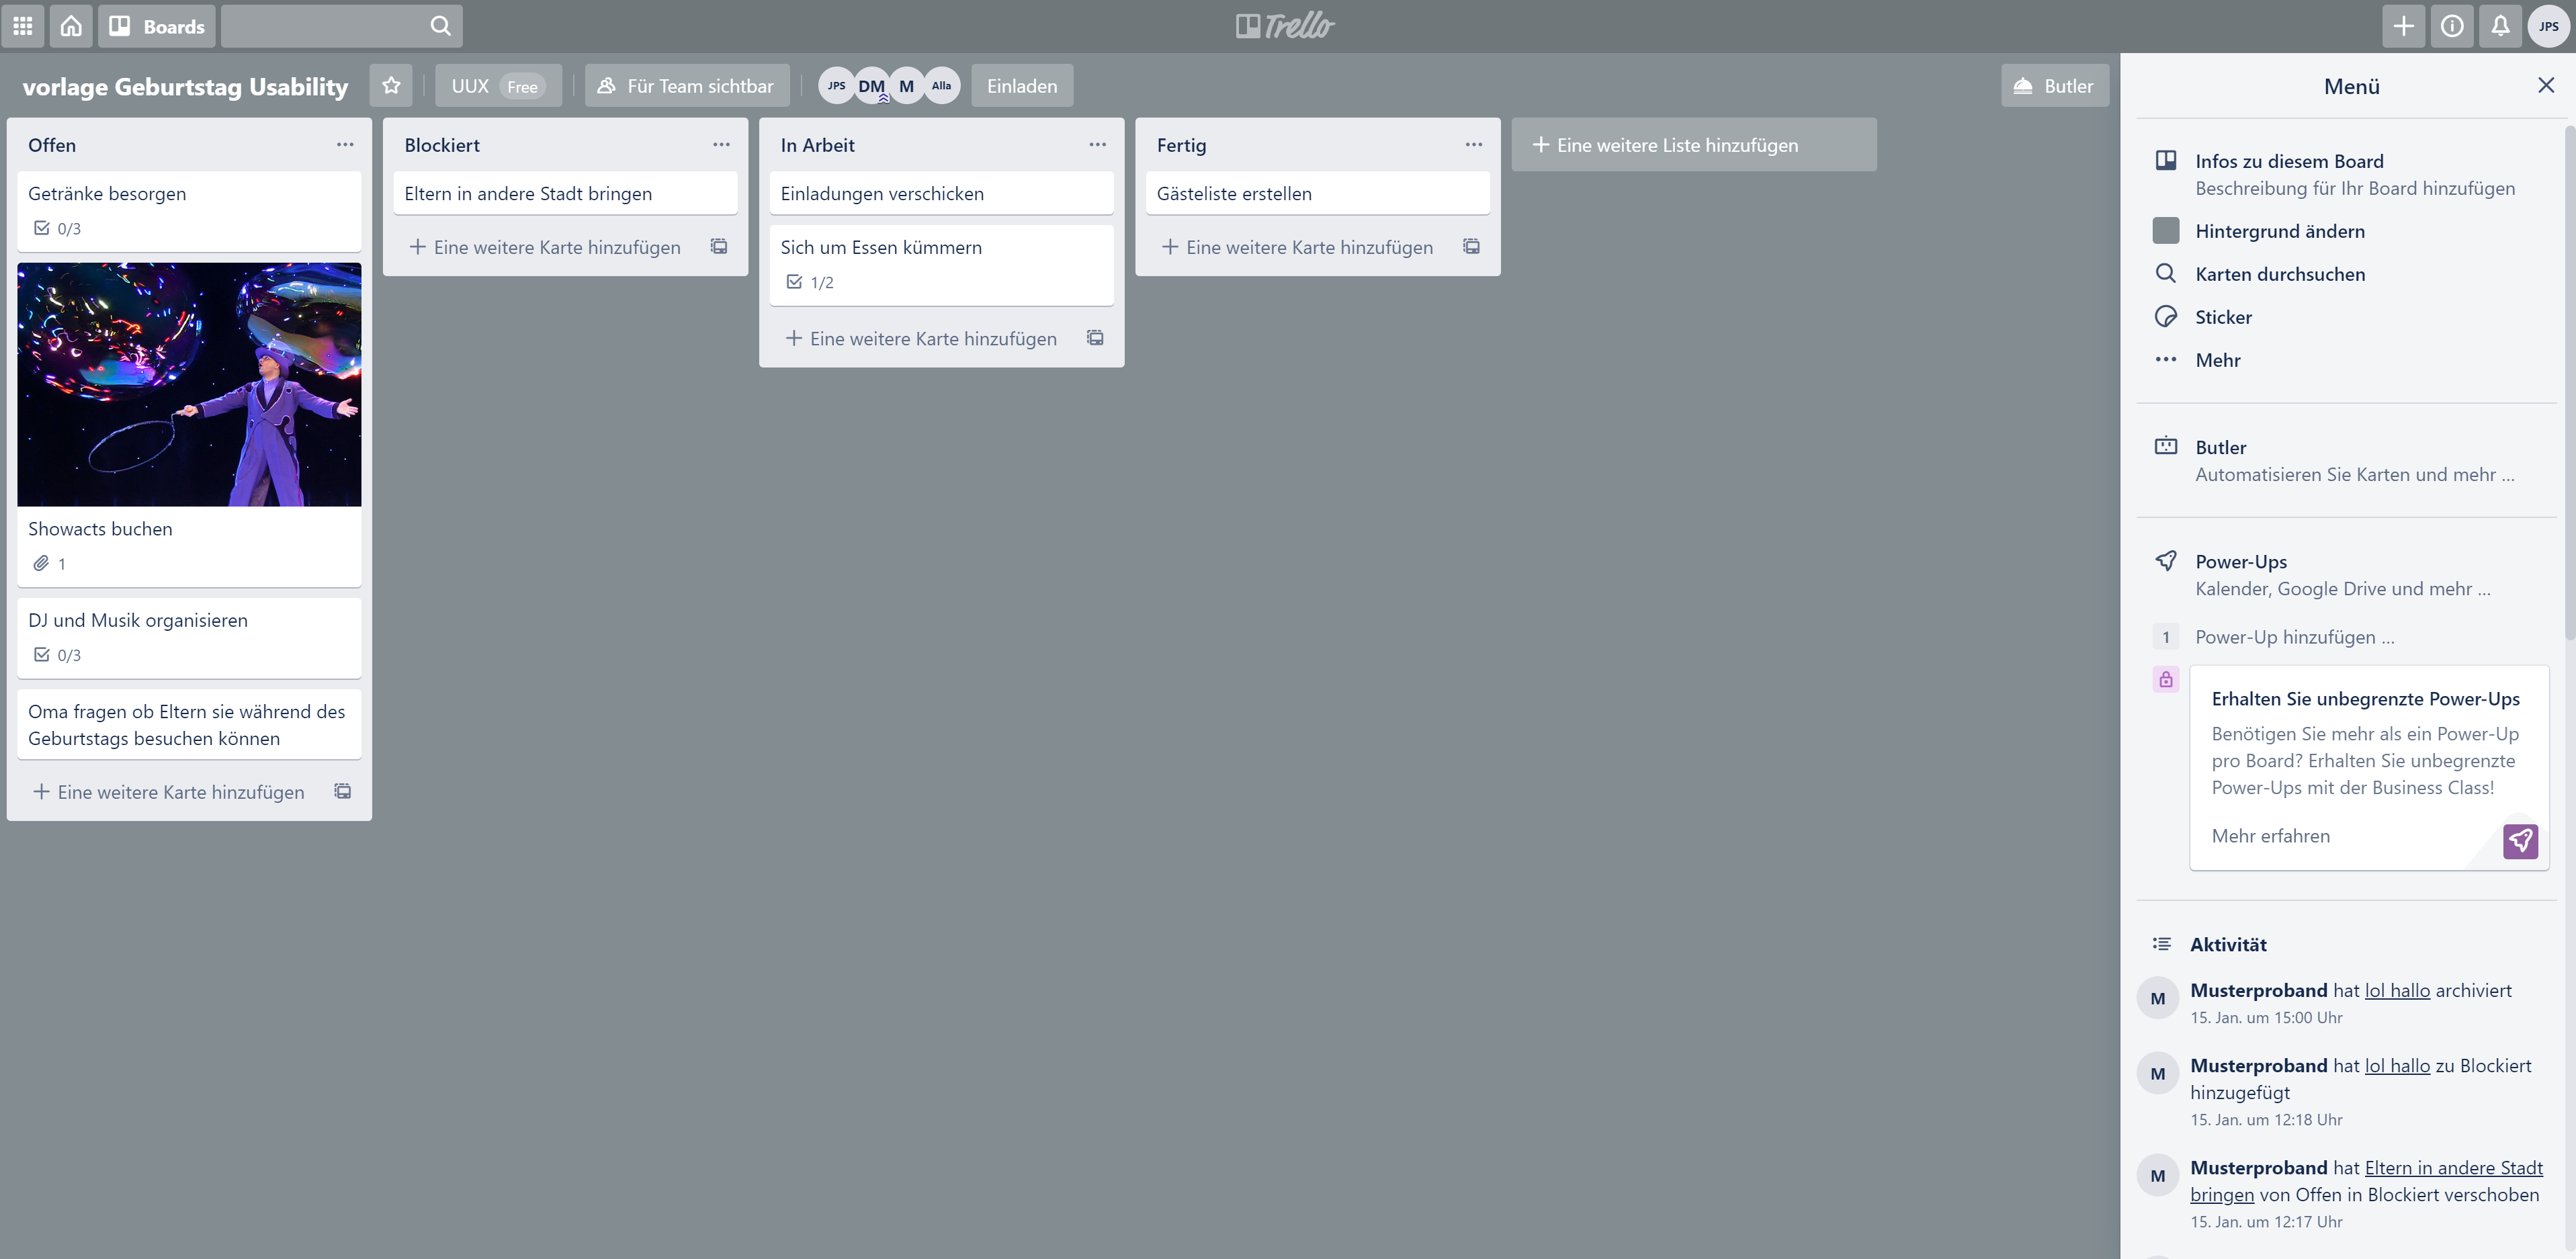
\includegraphics[width=\textwidth]{images/UI/Board Geburtstag.PNG}
    \centering
    \caption{Vorlagenboard 'Geburtstag' bei Trello}
    \label{fig:trellogebu}
\end{figure}

\begin{figure}[H]
    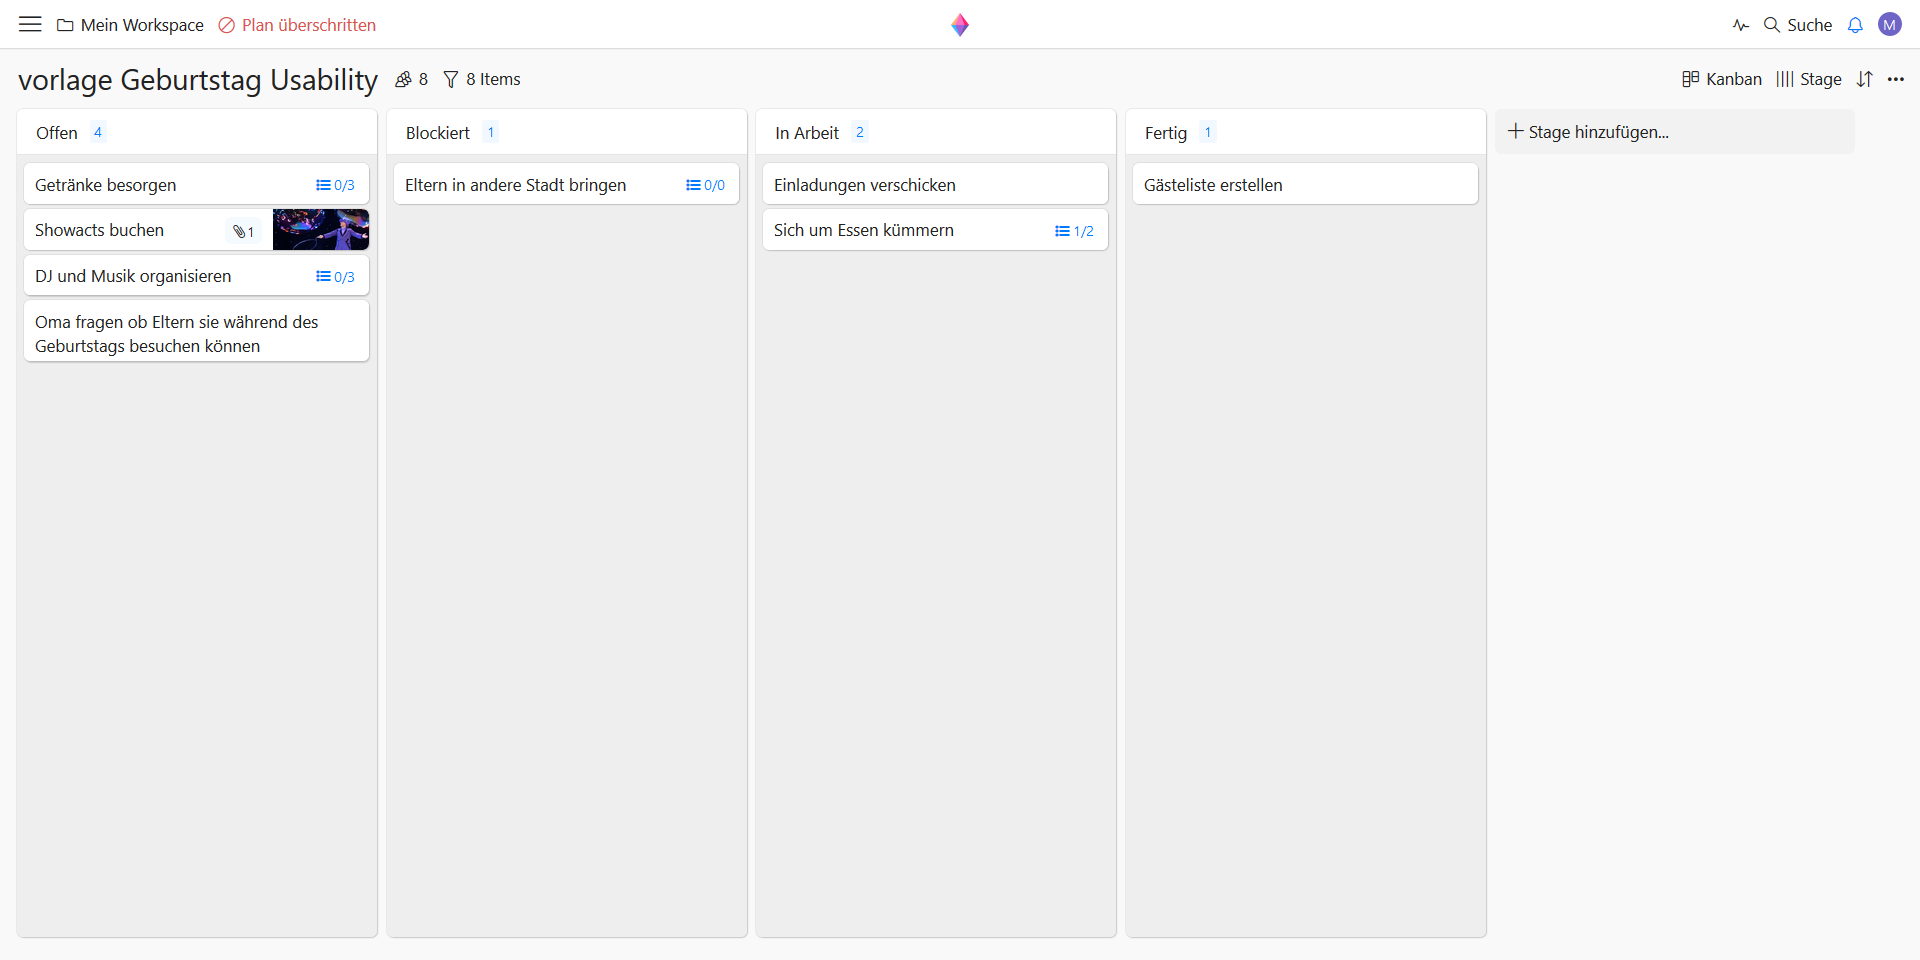
\includegraphics[width=\textwidth]{images/UI/geburtstagzenkit.PNG}
    \centering
    \caption{Vorlagenboard 'Geburtstag' bei Zenkit}
    \label{fig:zenkitgebu}
\end{figure}

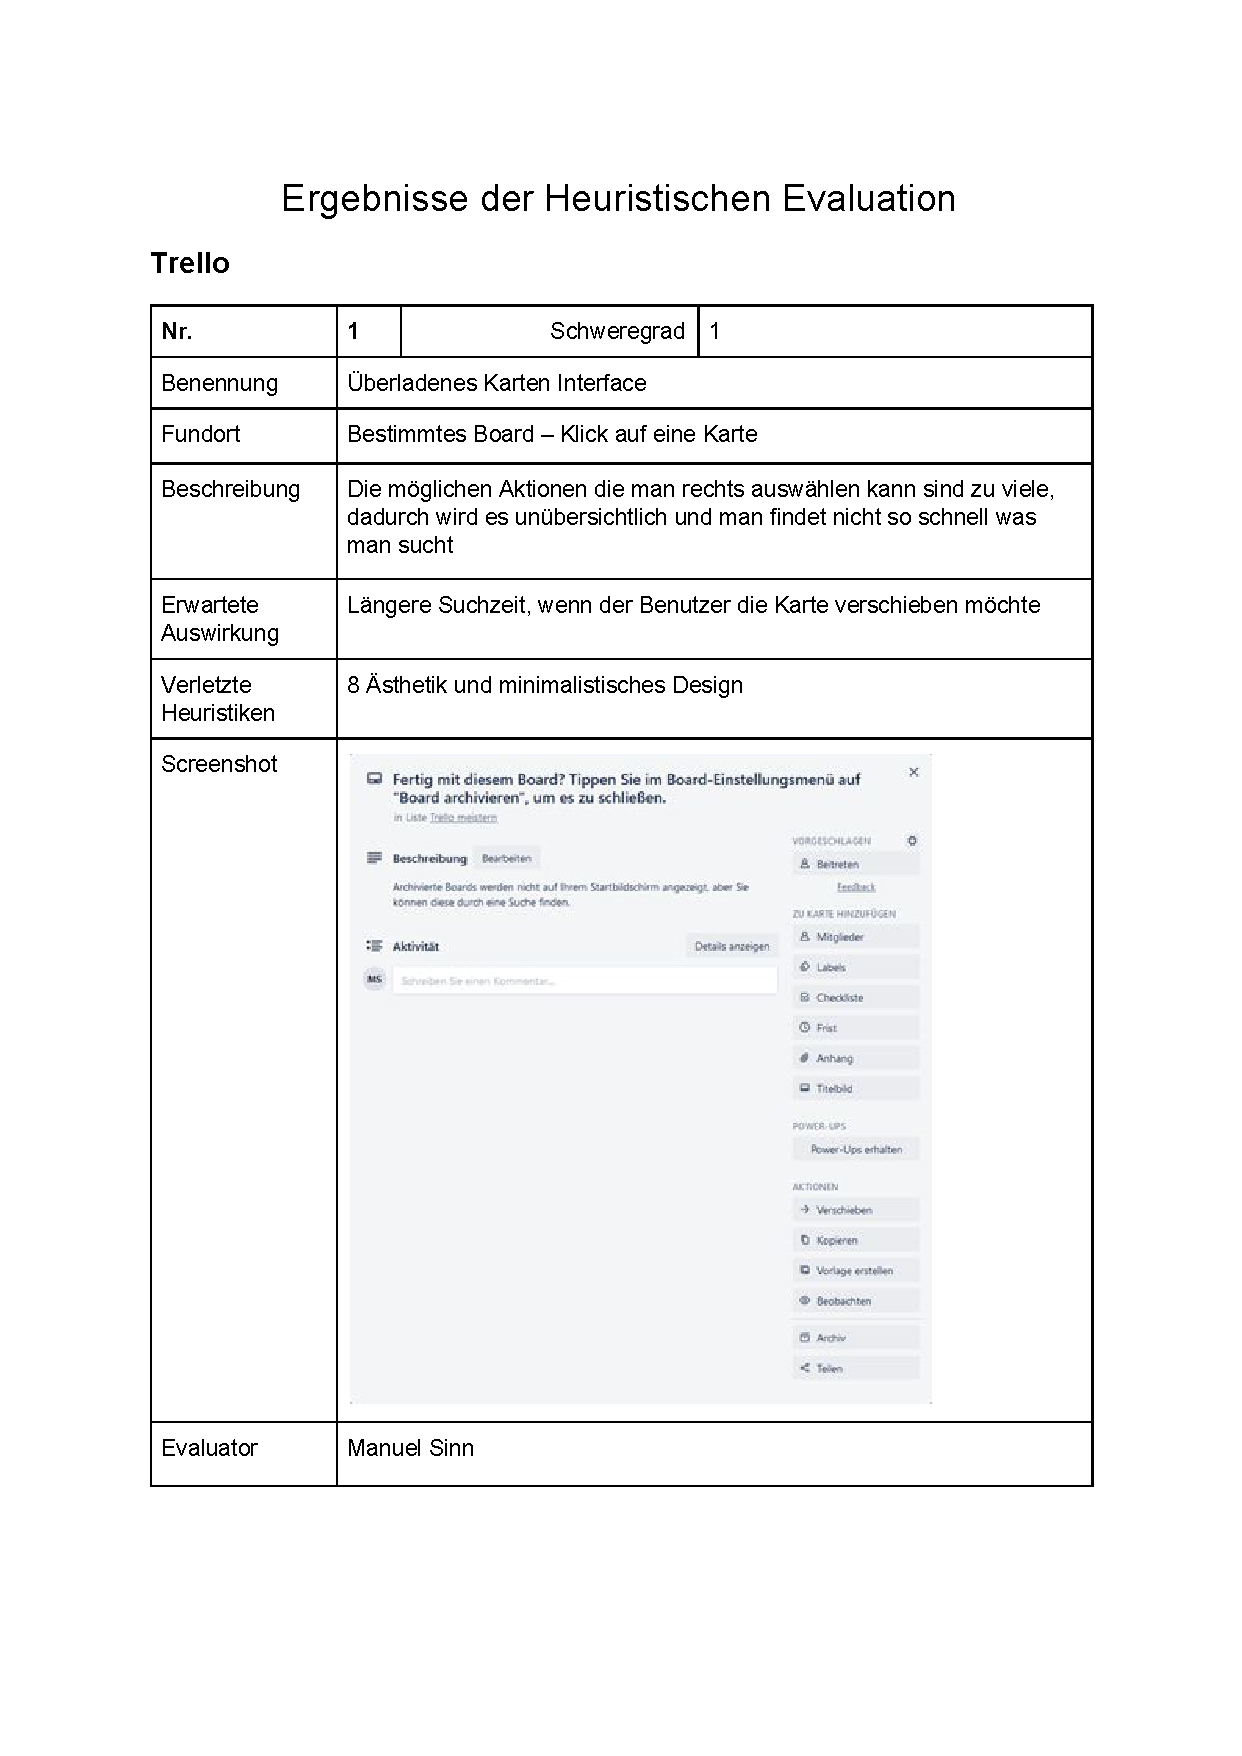
\includepdf[pages=1,scale=.9, pagecommand=\subsection{Ergebnisse}]{images/pdf/HE_Probleme.pdf}
\includepdf[pages=2-,scale=.9, pagecommand={}]{images/pdf/HE_Probleme.pdf}
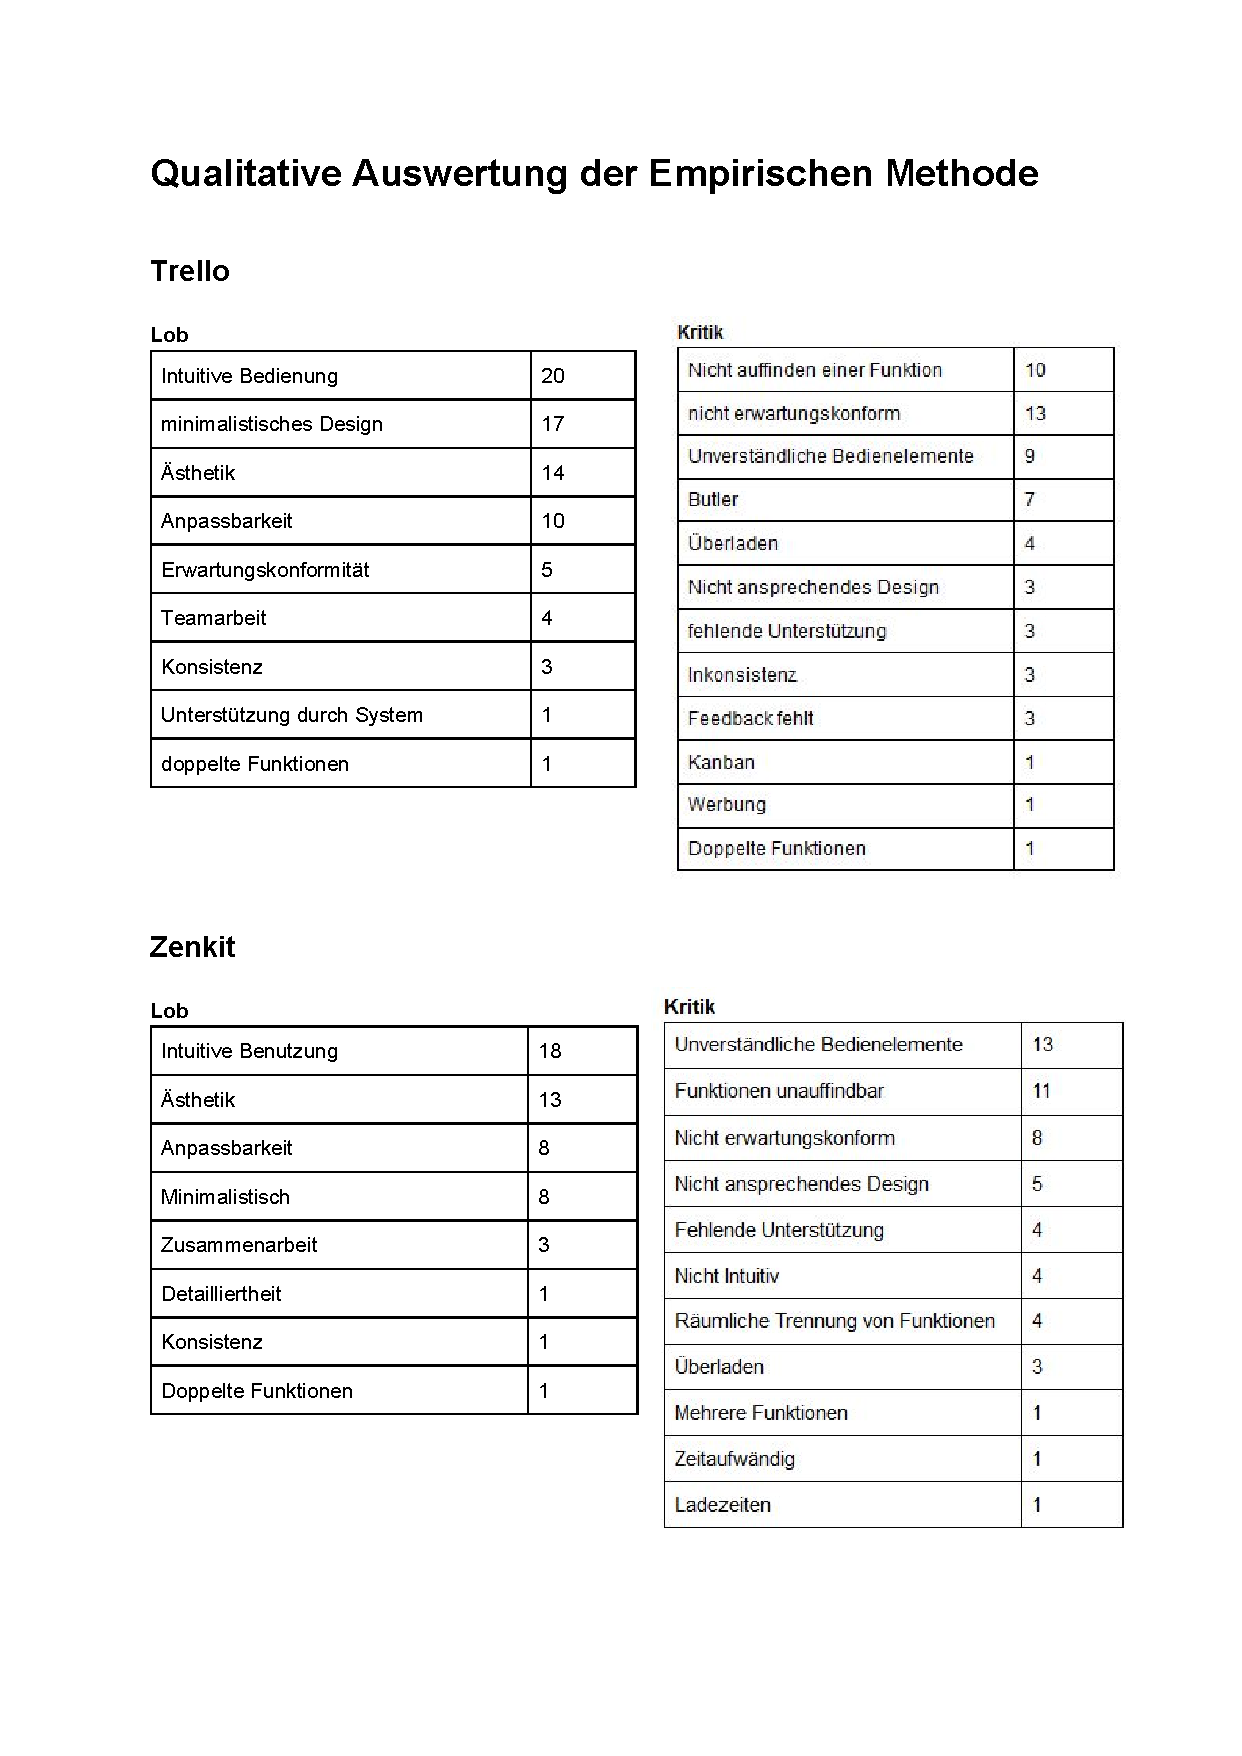
\includepdf[pages=-,scale=.8, pagecommand={}]{images/pdf/Quali_Auswertung.pdf}
\subsection{Sonstiges}

\begin{figure}[h]
    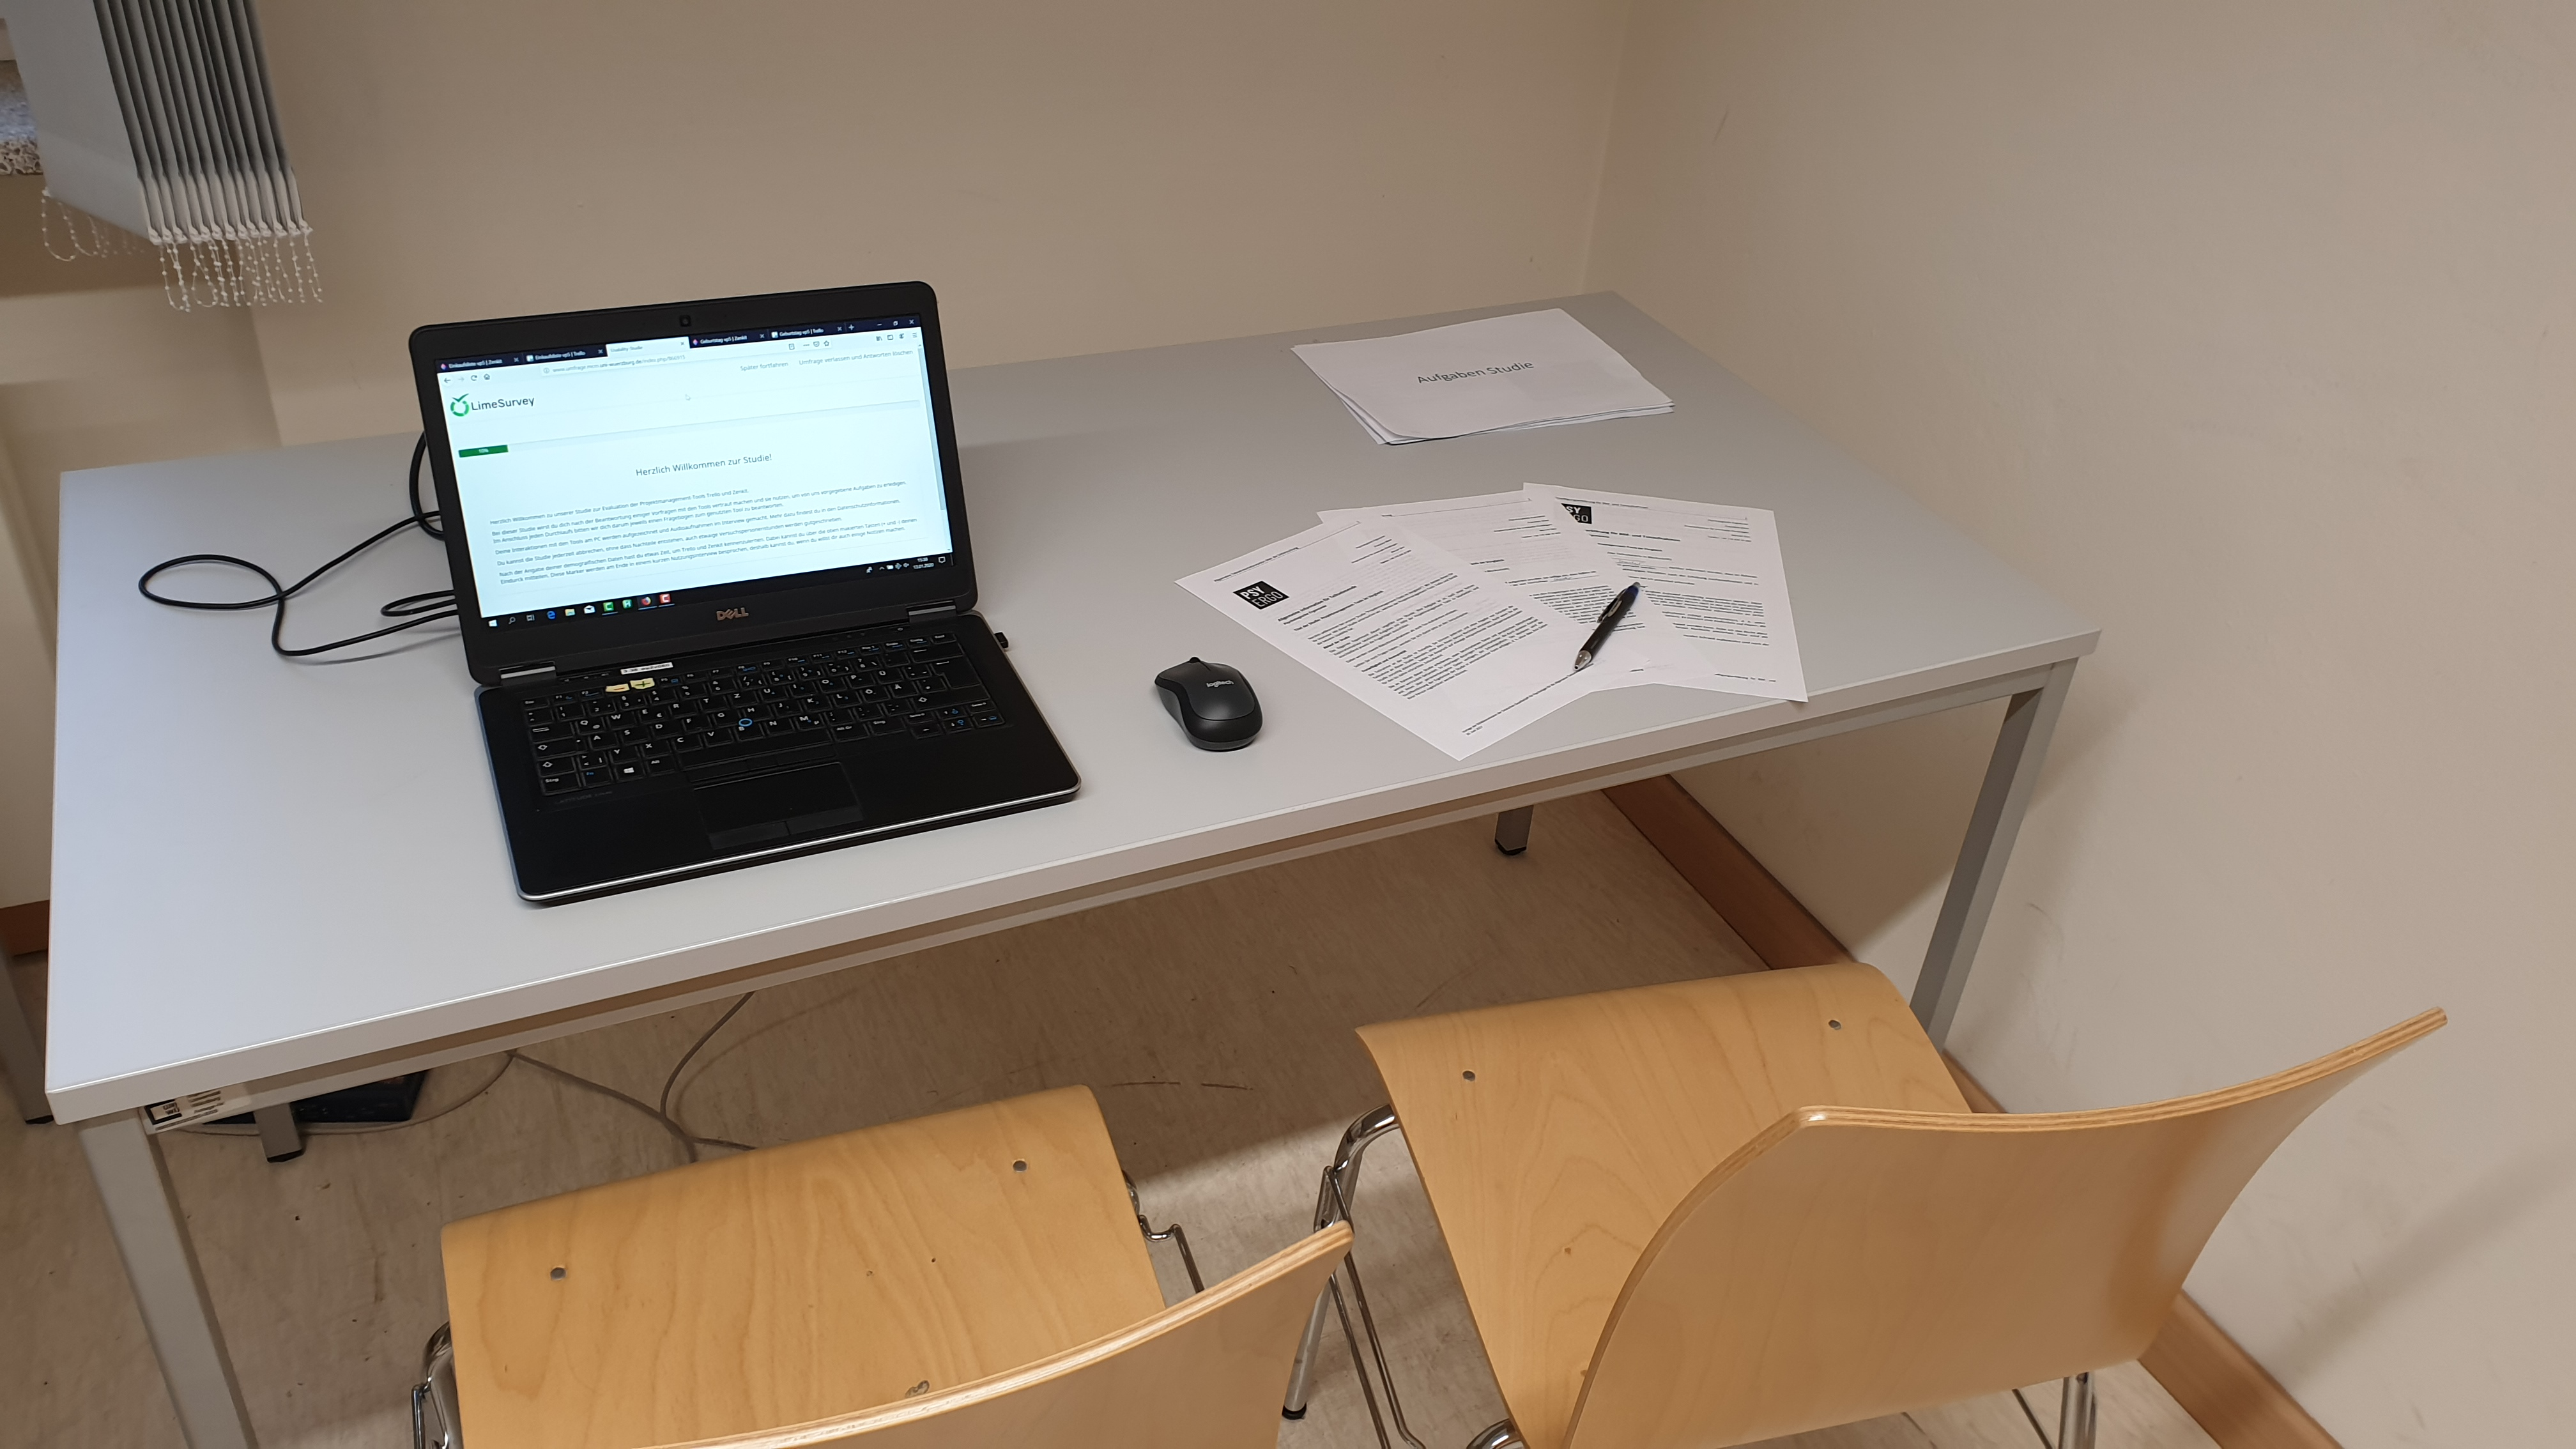
\includegraphics[width=0.9\textwidth]{images/Sonstiges/Studie-Aufbau.jpg}
    \centering
    \caption{Versuchssituation, wie sie die Versuchsperson zu Beginn der Studie vorfand}
    \label{fig:aufbau}
\end{figure}

\begin{figure}[h]
    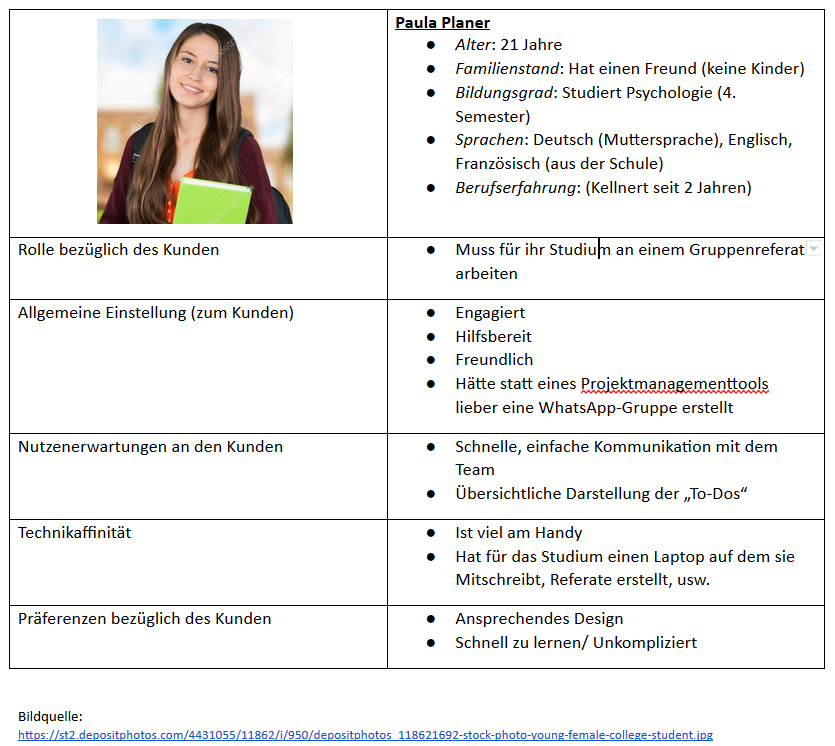
\includegraphics[width=0.7\textwidth]{images/Sonstiges/persona.PNG}
    \centering
    \caption{Persona, die als Hintergrund bzw. Ausgangspunkt für die Heuristische Evaluation genutzt wurde.}
    \label{fig:persona}
\end{figure}

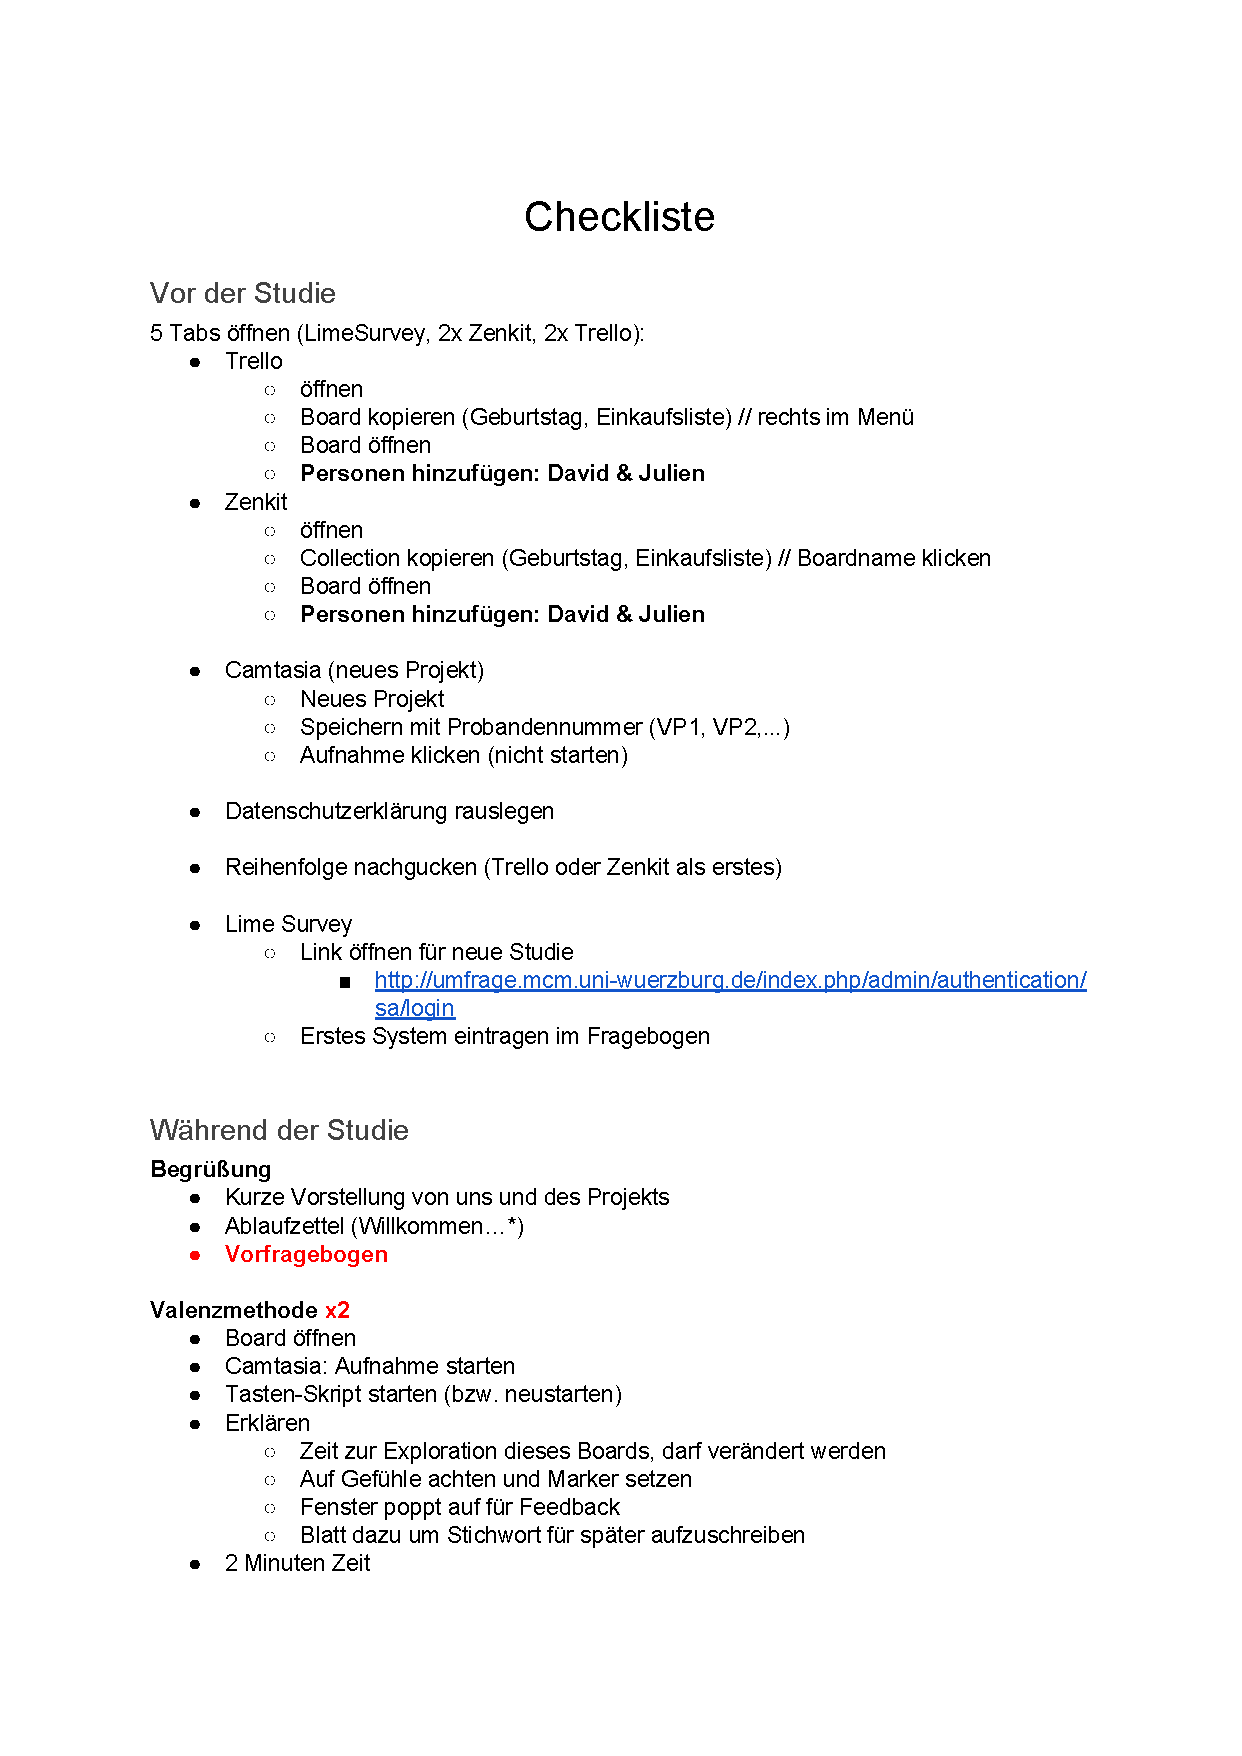
\includepdf[pages=-,scale=.8, pagecommand={}]{images/pdf/Checkliste.pdf}

\begin{figure}[h]
    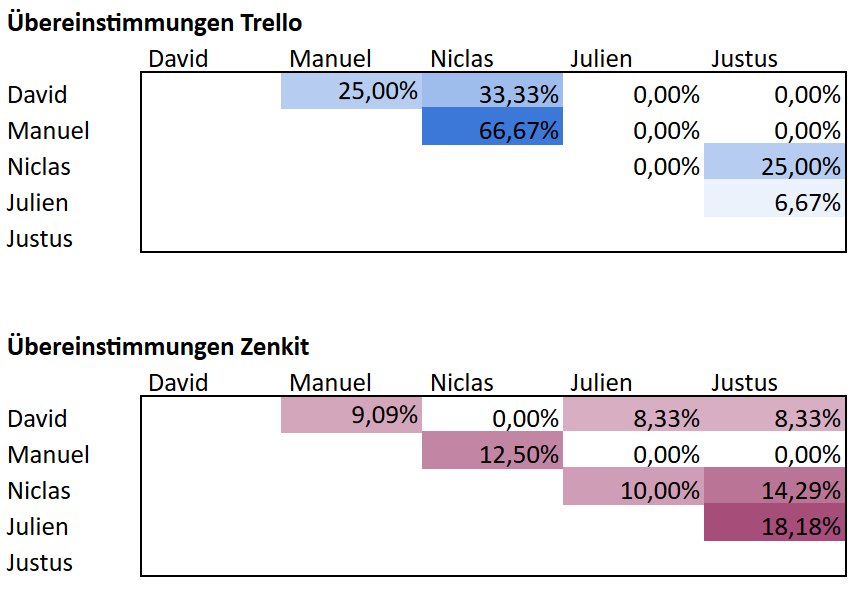
\includegraphics[width=0.7\textwidth]{images/Statistiken/uebereinstimmungen.PNG}
    \centering
    \caption{Übereinstimmungen zwischen den Evaluatoren bezüglich der gefundenen Probleme bei der Heuristischen Evaluation. Berechnet als Anteil der Probleme, die von beiden Evaluatoren gefunden wurden.}
    \label{fig:uebereinstimmungen}
\end{figure}

\begin{figure}[h]
    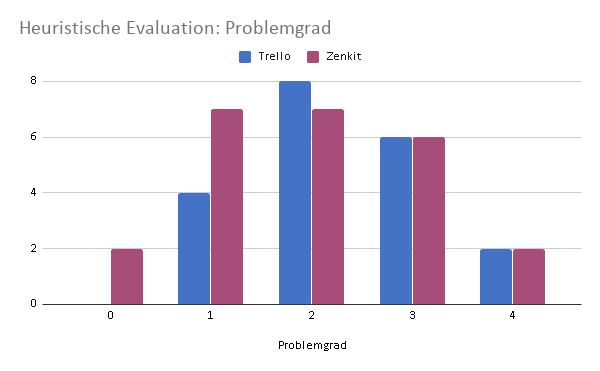
\includegraphics[width=0.8\textwidth]{images/Statistiken/problemgrad.png}
    \caption{Verteilung der gefundenen Probleme der Heuristischen Evaluation nach Problemgrad}
    \label{fig:gefundene_probleme}
\end{figure}

\begin{figure}[H]
    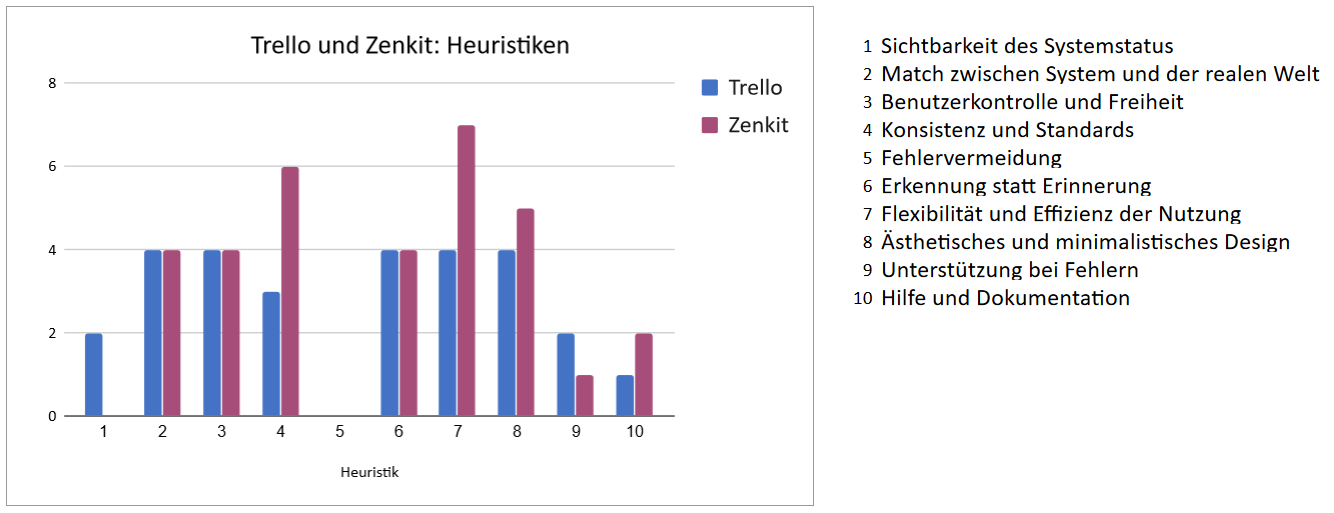
\includegraphics[width=0.9\textwidth]{images/Statistiken/probleme_heuristiken_neu.png}
    \centering
    \caption{Anzahl der gefundenen Probleme pro Heuristik}
    \label{fig:heuristik_probleme}
\end{figure}

\begin{figure}[h]
    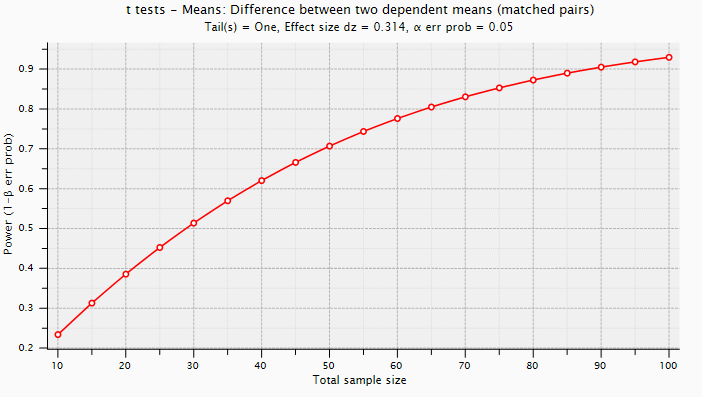
\includegraphics[width=0.7\textwidth]{images/Statistiken/powertlx.PNG}
    \centering
    \caption{Die Teststärke als Funktion der Stichprobengröße des NASA-TLX-Anstrengung Tests}
    \label{fig:powertlx}
\end{figure}


\begin{figure}[h]
    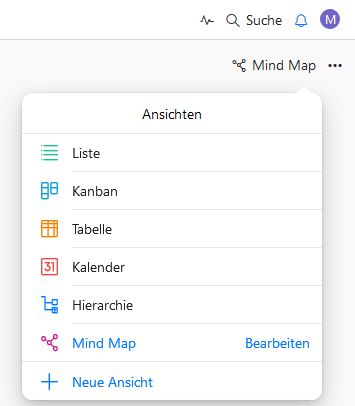
\includegraphics[width=0.4\textwidth]{images/UI/zenkit_ansichten.PNG}
    \centering
    \caption{Auswahl der möglichen Ansichten Zenkits neben des Kanban Standards}
    \label{fig:views}
\end{figure}

\FloatBarrier

\newpage
\bibliography{references}
\end{document}